\documentclass[12pt, spanish]{article}
\usepackage[spanish]{babel}
\selectlanguage{spanish}
%\usepackage{natbib}
\usepackage{url}
\usepackage[utf8x]{inputenc}
\usepackage{graphicx}
\graphicspath{{images/}}
\usepackage{parskip}
\usepackage{fancyhdr}
\usepackage{vmargin}
\usepackage{multirow}
\usepackage{float}
\usepackage{chngpage}
\usepackage{enumitem}

\usepackage{amsfonts}

\usepackage{subcaption}

\usepackage{hyperref}
\usepackage[
    type={CC},
    modifier={by-nc-sa},
    version={4.0},
]{doclicense}

\hypersetup{
    colorlinks=true,
    linkcolor=blue,
    filecolor=magenta,
    urlcolor=cyan,
}

% para codigo
\usepackage{listings}
\usepackage{xcolor}



%% configuración de listings

\definecolor{listing-background}{HTML}{F7F7F7}
\definecolor{listing-rule}{HTML}{B3B2B3}
\definecolor{listing-numbers}{HTML}{B3B2B3}
\definecolor{listing-text-color}{HTML}{000000}
\definecolor{listing-keyword}{HTML}{435489}
\definecolor{listing-identifier}{HTML}{435489}
\definecolor{listing-string}{HTML}{00999A}
\definecolor{listing-comment}{HTML}{8E8E8E}
\definecolor{listing-javadoc-comment}{HTML}{006CA9}

\lstdefinestyle{eisvogel_listing_style}{
  language         = python,
%$if(listings-disable-line-numbers)$
%  xleftmargin      = 0.6em,
%  framexleftmargin = 0.4em,
%$else$
  numbers          = left,
  xleftmargin      = 0em,
 framexleftmargin = 0em,
%$endif$
  backgroundcolor  = \color{listing-background},
  basicstyle       = \color{listing-text-color}\small\ttfamily{}\linespread{1.15}, % print whole listing small
  breaklines       = true,
  frame            = single,
  framesep         = 0.19em,
  rulecolor        = \color{listing-rule},
  frameround       = ffff,
  tabsize          = 4,
  numberstyle      = \color{listing-numbers},
  aboveskip        = 1.0em,
  belowskip        = 0.1em,
  abovecaptionskip = 0em,
  belowcaptionskip = 1.0em,
  keywordstyle     = \color{listing-keyword}\bfseries,
  classoffset      = 0,
  sensitive        = true,
  identifierstyle  = \color{listing-identifier},
  commentstyle     = \color{listing-comment},
  morecomment      = [s][\color{listing-javadoc-comment}]{/**}{*/},
  stringstyle      = \color{listing-string},
  showstringspaces = false,
  escapeinside     = {/*@}{@*/}, % Allow LaTeX inside these special comments
  literate         =
  {á}{{\'a}}1 {é}{{\'e}}1 {í}{{\'i}}1 {ó}{{\'o}}1 {ú}{{\'u}}1
  {Á}{{\'A}}1 {É}{{\'E}}1 {Í}{{\'I}}1 {Ó}{{\'O}}1 {Ú}{{\'U}}1
  {à}{{\`a}}1 {è}{{\'e}}1 {ì}{{\`i}}1 {ò}{{\`o}}1 {ù}{{\`u}}1
  {À}{{\`A}}1 {È}{{\'E}}1 {Ì}{{\`I}}1 {Ò}{{\`O}}1 {Ù}{{\`U}}1
  {ä}{{\"a}}1 {ë}{{\"e}}1 {ï}{{\"i}}1 {ö}{{\"o}}1 {ü}{{\"u}}1
  {Ä}{{\"A}}1 {Ë}{{\"E}}1 {Ï}{{\"I}}1 {Ö}{{\"O}}1 {Ü}{{\"U}}1
  {â}{{\^a}}1 {ê}{{\^e}}1 {î}{{\^i}}1 {ô}{{\^o}}1 {û}{{\^u}}1
  {Â}{{\^A}}1 {Ê}{{\^E}}1 {Î}{{\^I}}1 {Ô}{{\^O}}1 {Û}{{\^U}}1
  {œ}{{\oe}}1 {Œ}{{\OE}}1 {æ}{{\ae}}1 {Æ}{{\AE}}1 {ß}{{\ss}}1
  {ç}{{\c c}}1 {Ç}{{\c C}}1 {ø}{{\o}}1 {å}{{\r a}}1 {Å}{{\r A}}1
  {€}{{\EUR}}1 {£}{{\pounds}}1 {«}{{\guillemotleft}}1
  {»}{{\guillemotright}}1 {ñ}{{\~n}}1 {Ñ}{{\~N}}1 {¿}{{?`}}1
  {…}{{\ldots}}1 {≥}{{>=}}1 {≤}{{<=}}1 {„}{{\glqq}}1 {“}{{\grqq}}1
  {”}{{''}}1
}
\lstset{style=eisvogel_listing_style}


\usepackage[default]{sourcesanspro}

\setmarginsrb{2 cm}{1 cm}{2 cm}{2 cm}{1 cm}{1.5 cm}{1 cm}{1.5 cm}

\title{Práctica 2:\\
Modelos de Monte Carlo. Generadores de datos.\hspace{0.05cm} }
\author{Antonio David Villegas Yeguas}
\date{\today}

\renewcommand*\contentsname{hola}

\makeatletter
\let\thetitle\@title
\let\theauthor\@author
\let\thedate\@date
\makeatother

\pagestyle{fancy}
\fancyhf{}
\rhead{\theauthor}
\lhead{\thetitle}
\cfoot{\thepage}

\begin{document}

%%%%%%%%%%%%%%%%%%%%%%%%%%%%%%%%%%%%%%%%%%%%%%%%%%%%%%%%%%%%%%%%%%%%%%%%%%%%%%%%%%%%%%%%%

\begin{titlepage}
    \centering
    \vspace*{0.3 cm}
    
\includegraphics[scale = 0.50]{ugr.png}\\[0.7 cm]
    %\textsc{\LARGE Universidad de Granada}\\[2.0 cm]
    \textsc{\large 4º CSI 2020/21 - Grupo 1}\\[0.5 cm]
    \textsc{\large Grado en Ingeniería Informática}\\[0.5 cm]
    \rule{\linewidth}{0.2 mm} \\[0.2 cm]
    { \huge \bfseries \thetitle}\\
    \rule{\linewidth}{0.2 mm} \\[1 cm]

    \begin{minipage}{0.4\textwidth}
        \begin{flushleft} \large
            \emph{Autor:}\\
            \theauthor\\
			 \emph{DNI:}\\
            77021623-M
            \end{flushleft}
            \end{minipage}~
            \begin{minipage}{0.4\textwidth}
            \begin{flushright} \large
            \emph{Asignatura: \\
            Simulación de Sistemas}   \\
            \emph{Correo:}\\
            advy99@correo.ugr.es
        \end{flushright}
    \end{minipage}\\[0.5cm]

    {\large \thedate}\\[0.5cm]
    %{\url{https://github.com/advy99/AA/}}
    {\doclicenseThis}

    \vfill

\end{titlepage}

%%%%%%%%%%%%%%%%%%%%%%%%%%%%%%%%%%%%%%%%%%%%%%%%%%%%%%%%%%%%%%%%%%%%%%%%%%%%%%%%%%%%%%%%%

\tableofcontents
\pagebreak

%%%%%%%%%%%%%%%%%%%%%%%%%%%%%%%%%%%%%%%%%%%%%%%%%%%%%%%%%%%%%%%%%%%%%%%%%%%%%%%%%%%%%%%%%


\section*{Introducción}

En esta práctica continuaremos con la implementación de modelos de Montecarlo, así como comenzar a trabajar e implementar con generadores de datos.

Esta práctica consta de dos partes, una primera parte centrada en la implementación de un modelo de Montecarlo que utilizará tres generadores de datos distintos, todos ellos basados en el método de tablas de búsqueda, sin embargo cada generador seguirá una distribución distinta.

La segunda parte se centrará en los propios generadores de datos. En esta parte mejoraremos el comportamiento de los generadores utilizados en la primera parte, además de implementar nuestros propios generadores de datos, que a pesar de implementar generadores simples, servirá como introducción al funcionamiento y uso de generadores de datos, principalmente en su importancia y como construir generadores de datos eficientes.


\section{Mi segundo modelo de simulación de Montecarlo}

Para este segundo modelo de simulación de Montecarlo nos centraremos en el problema de quioscos de periódicos. Cierto establecimiento se abastece diariamente de un producto que vende diariamente, por ejemplo un quiosco que vende periodicos, sin embargo, el número de periódicos que compra diariamente a la editorial se establece en un contrato a largo plazo y no puede ser modificado. El establecimiento, por cada venta, obtiene una ganancia de $x$ euros, sin embargo también obtiene una pérdida de $y$ por cada unidad no vendida en el día. El establecimiento también conoce la distribución de probabilidad con la que vende periódicos. Con estos datos, este sistema estudiará el valor óptimo de periódicos $s$ que han de contratarse para que el quiosco tenga una ganancia máxima.

En todo momento la simulación tendrá en cuenta valores de demanda de entre 0 y 100 periódicos.

\subsection{Distribuciones de la demanda diaria}

Para estudiar este sistema se nos proponen tres distribuciones de probabilidad distintas:

\begin{enumerate}[label=\alph*]
	\item Distribución uniforme: La probabilidad de que se venda una cantidad $d$ de periódicos es la misma para cualquier $d$.
	\item Distribución proporcional: La probabilidad de que se venda una cantidad $d$ de periódicos es proporcional a $100 - d$
	\item Distribución triangular: La probabilidad de que se venda una cantidad $d$ de periódicos es proporcional a $d$ si $0 \leq d < 50$ y proporcional a $100 - d$ si $50 \leq d < 100$

\end{enumerate}



\subsection{Construcción del modelo}

De cara a estudiar el problema, construiremos un modelo de Montecarlo que, para todos los posibles valores de periódicos a contratadar ($s$ de 0 a 100), generen un número de veces una demanda a partir de la distribución que estemos estudiando, y con ese valor obtener la ganancia, con el objetivo de, tras un gran número de ejecuciones, realizar una buena estimación del valor óptimo.


Para probar el modelo se han realizado distintas ejecuciones, con distintos número de veces de generación de demanda. En concreto he realizado pruebas para $x = 10$ e $y = 1, y = 5, y = 10, y = 15$, con distintos valores de repetición, 100, 1000, 5000, 10000, 100000, 150000.

Tras realizar las distintas ejecuciones, obtenemos estos resultados:


\subsubsection{Resultados obtenidos con la distribución a}

La distribución a se basa en una distribución de probabilidad uniforme, es decir, todos los valores de demanda tienen las mismas probabilidades de aparecer.

\begin{figure}[H]
	\centering
	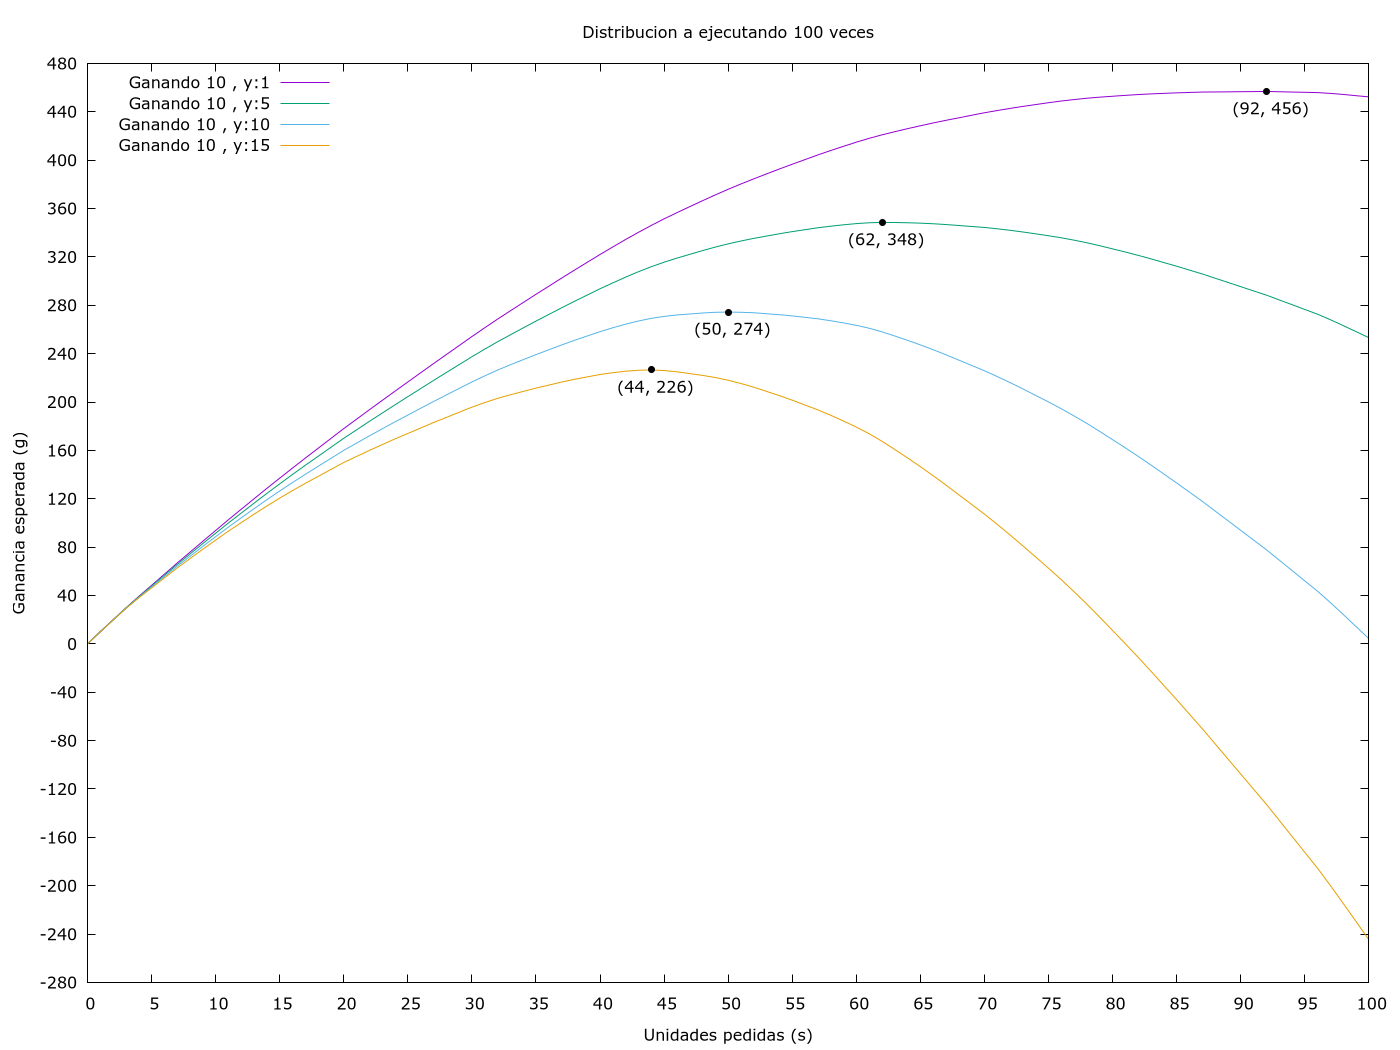
\includegraphics[scale = 0.2]{prob_a/datos_a_100.png}
	\caption{Con 100 repeticiones y la distribución a.}
	\label{fig:ej1_a_100}

\end{figure}

\begin{figure}[H]
	\centering
	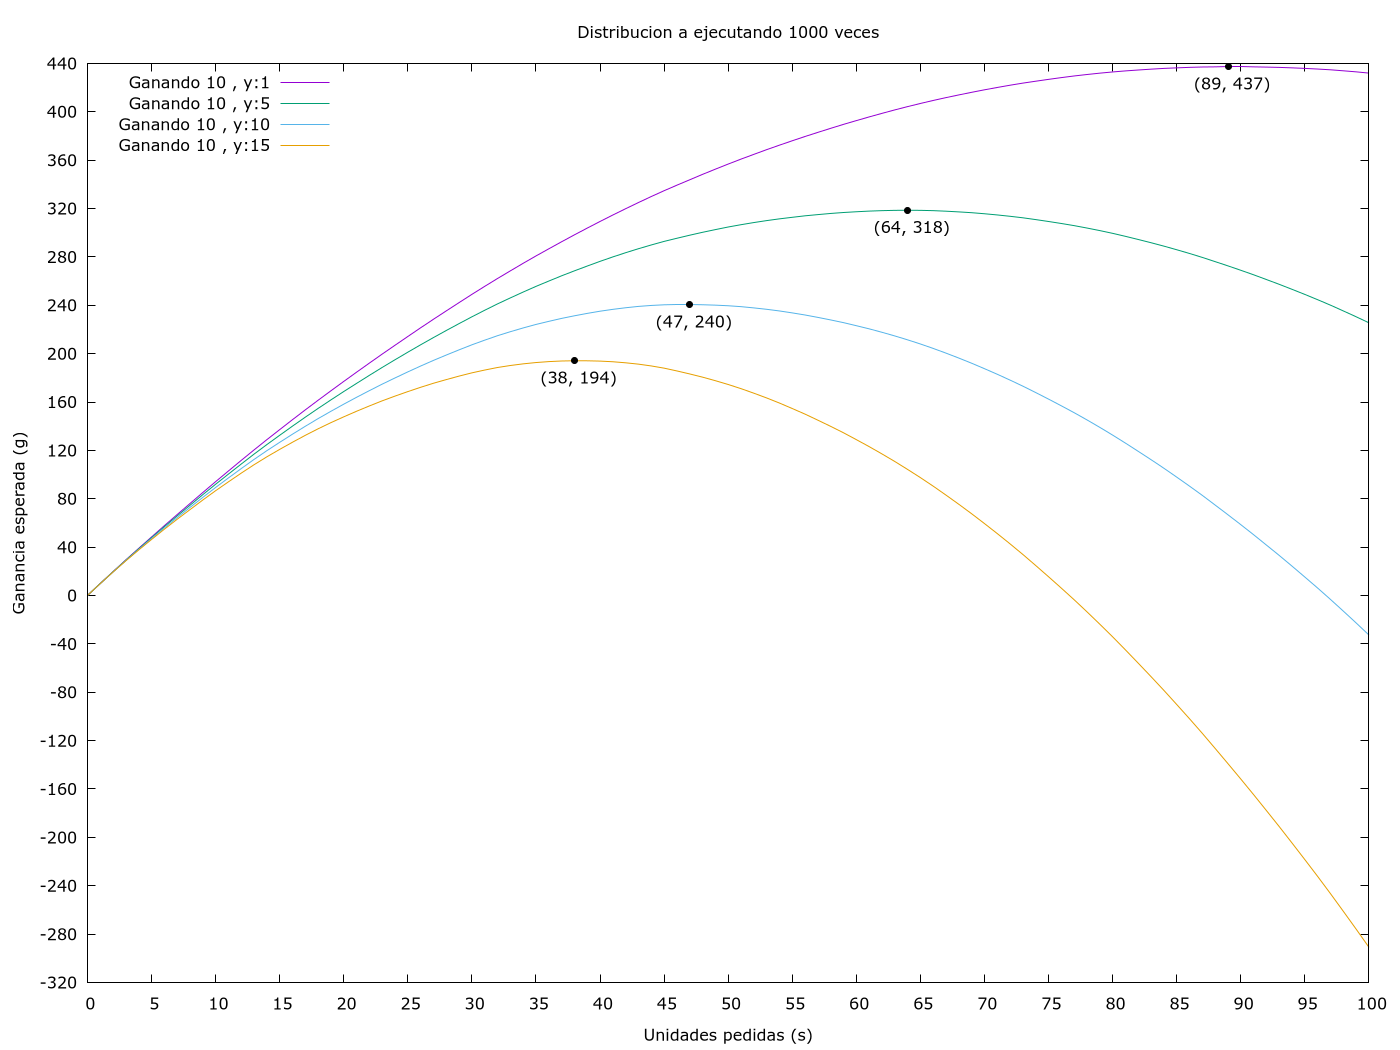
\includegraphics[scale = 0.2]{prob_a/datos_a_1000.png}
	\caption{Con 1000 repeticiones y la distribución a.}
	\label{fig:ej1_a_1000}

\end{figure}

\begin{figure}[H]
	\centering
	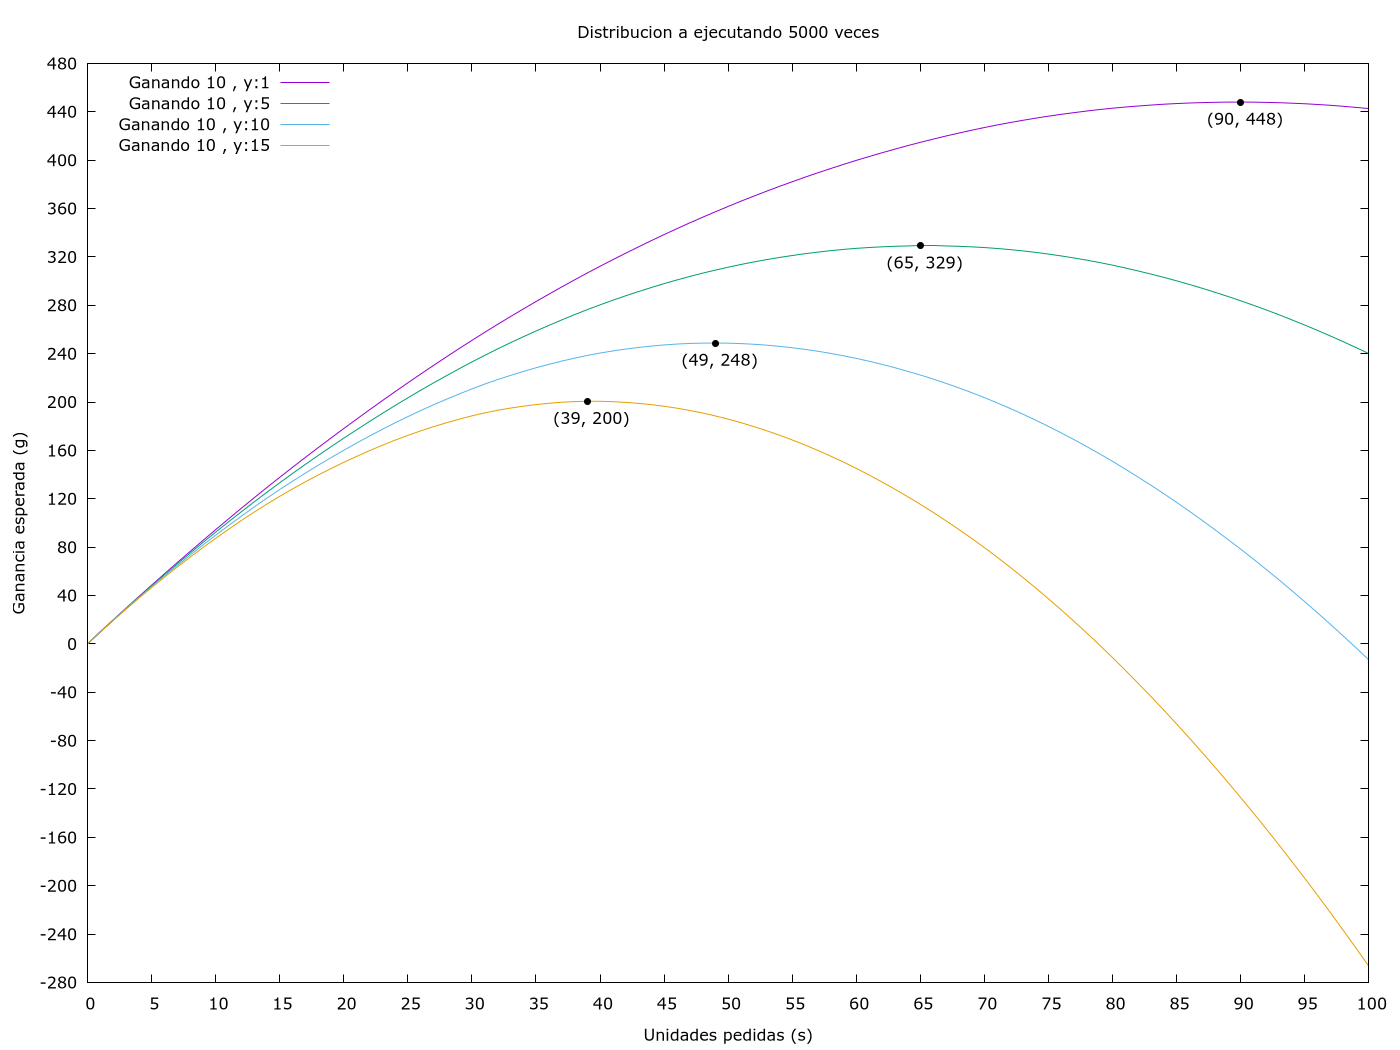
\includegraphics[scale = 0.2]{prob_a/datos_a_5000.png}
	\caption{Con 5000 repeticiones y la distribución a.}
	\label{fig:ej1_a_5000}

\end{figure}


\begin{figure}[H]
	\centering
	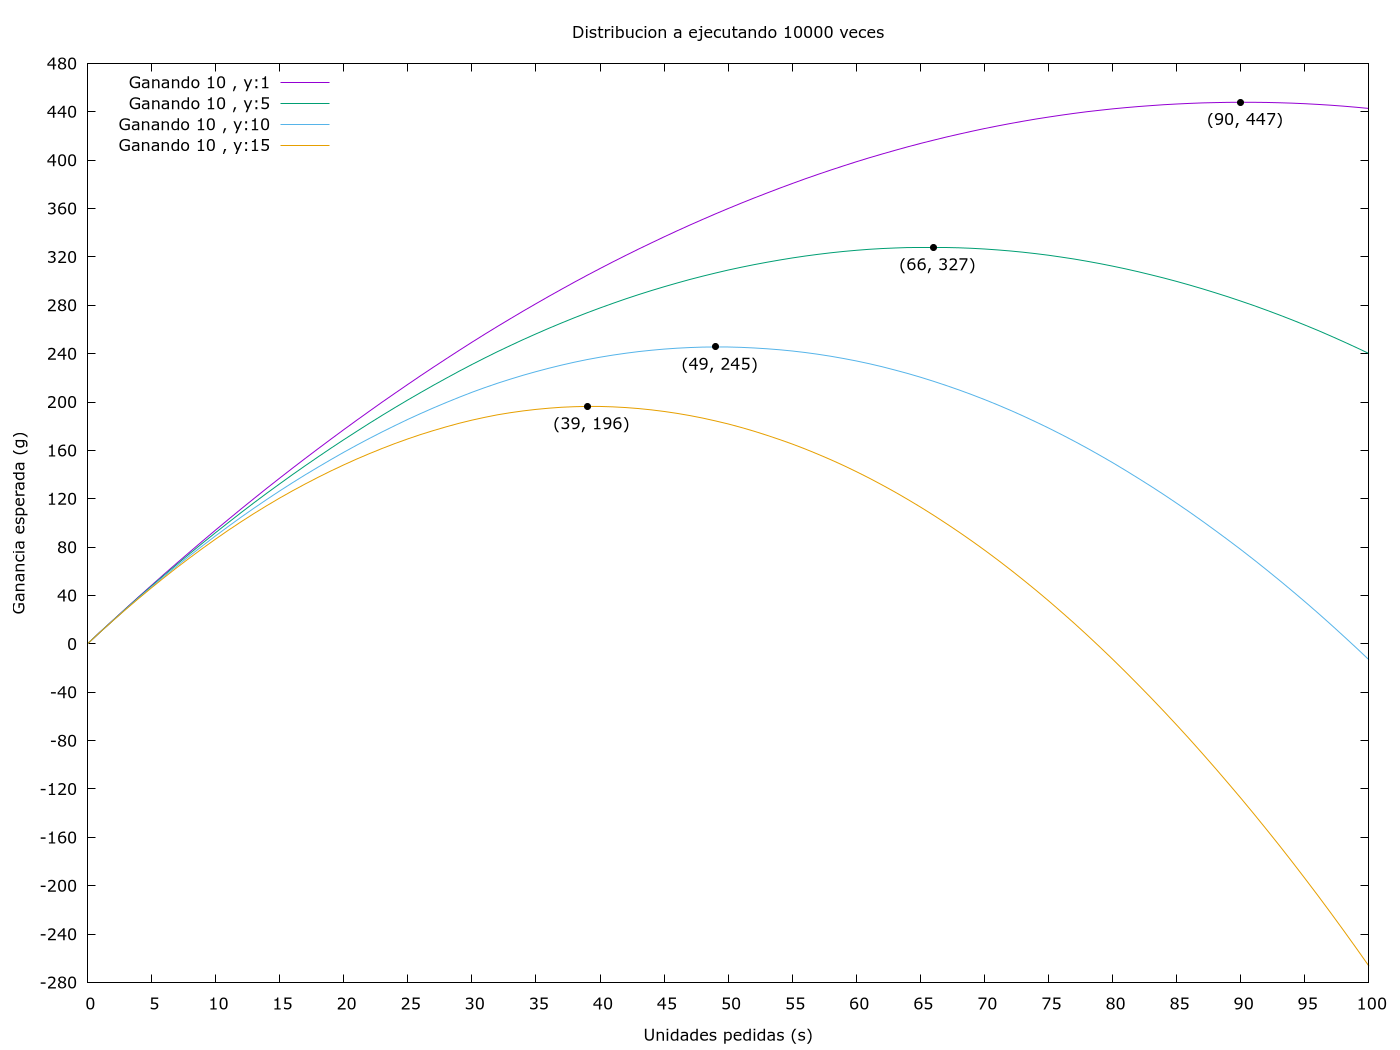
\includegraphics[scale = 0.2]{prob_a/datos_a_10000.png}
	\caption{Con 10000 repeticiones y la distribución a.}
	\label{fig:ej1_a_10000}

\end{figure}

\begin{figure}[H]
	\centering
	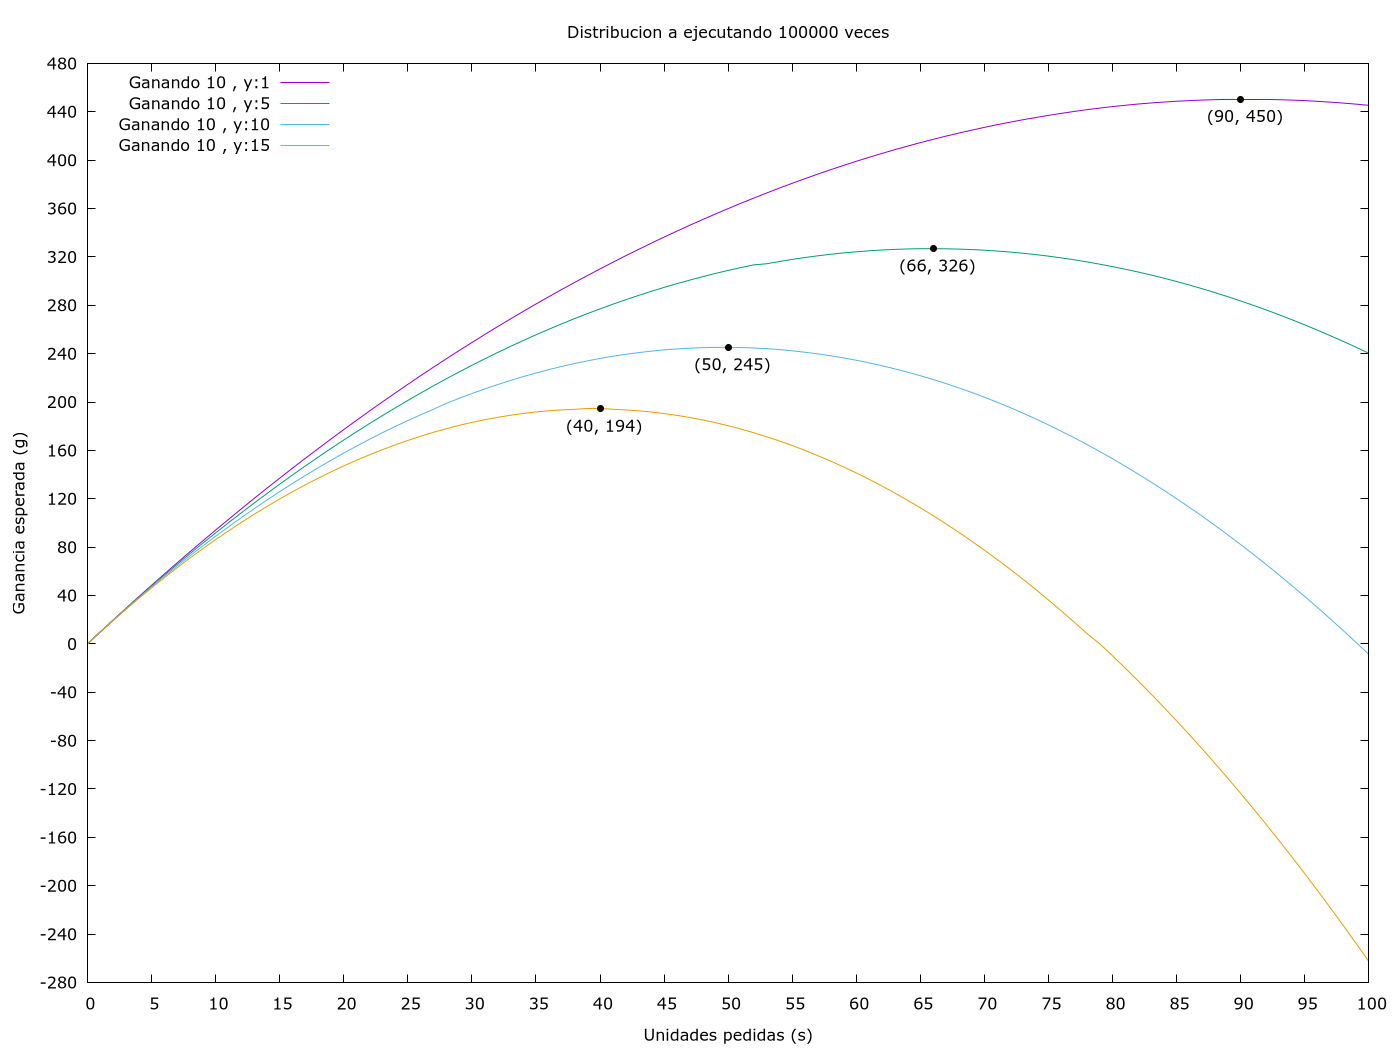
\includegraphics[scale = 0.2]{prob_a/datos_a_100000.png}
	\caption{Con 100000 repeticiones y la distribución a.}
	\label{fig:ej1_a_100000}

\end{figure}

\begin{figure}[H]
	\centering
	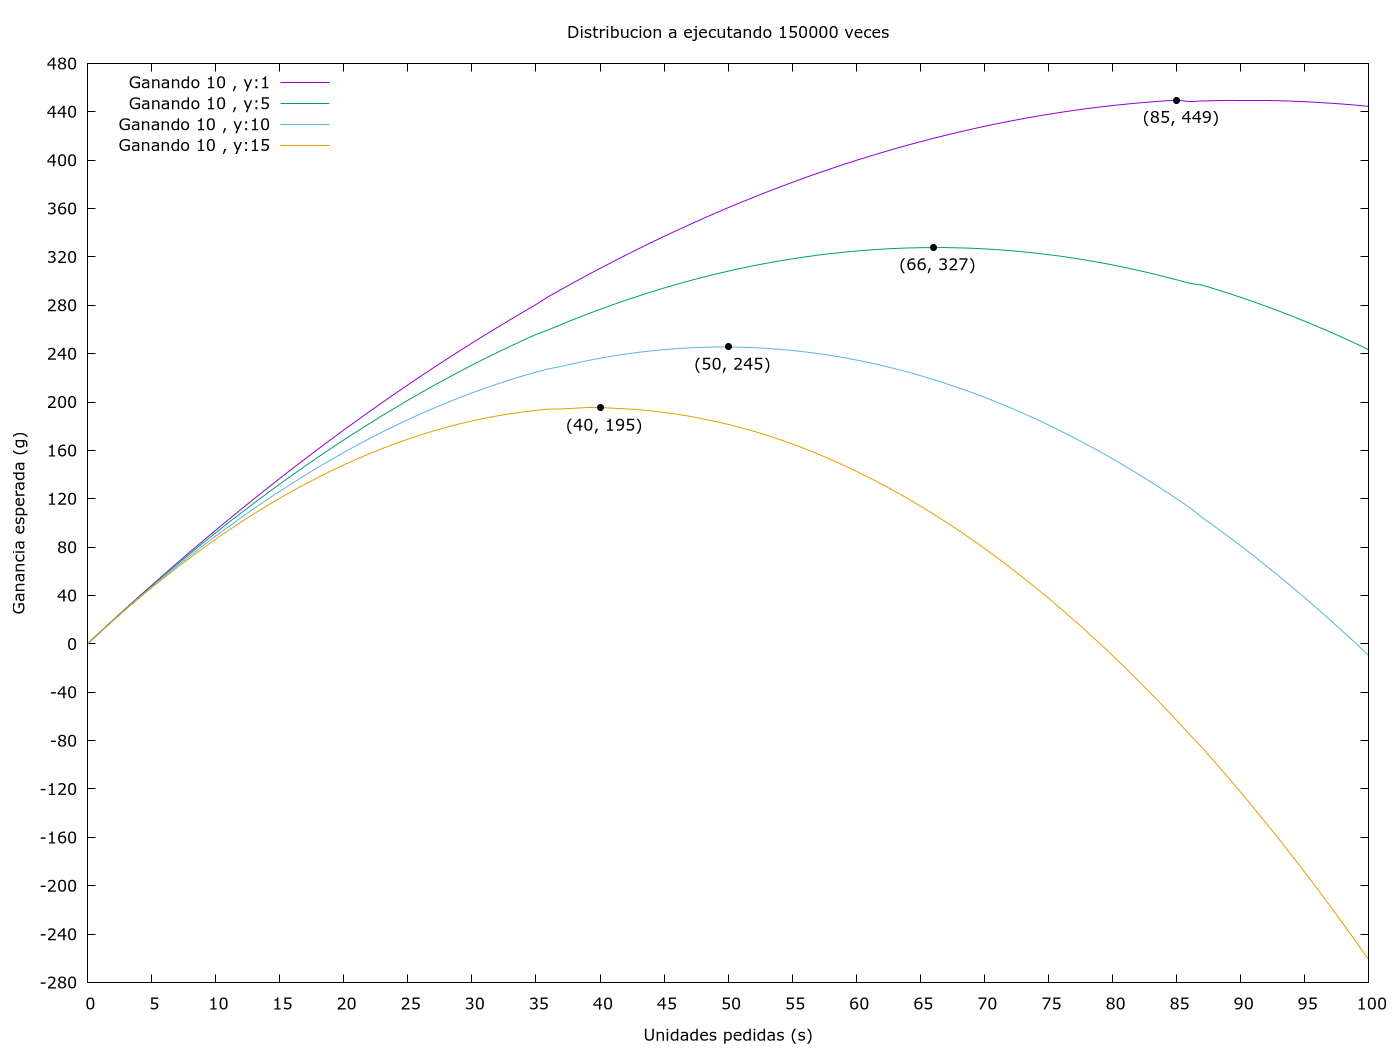
\includegraphics[scale = 0.2]{prob_a/datos_a_150000.png}
	\caption{Con 150000 repeticiones y la distribución a.}
	\label{fig:ej1_a_150000}

\end{figure}

En estas gráficas vemos como al ejecutar con distinto número de repeticiones, a mayor número de repeticiones se acerca más al óptimo calculado en el guión de la práctica hasta alcanzarlo, además de que en todas las gráficas, a una mayor perdida por unidad no vendida la ganancia máxima va siendo más baja y el óptimo de periódicos a contratar se acerca a cero, por lo que es el comportamiento esperado del sistema.

En este caso, en el que cualquier valor de demanda tiene la misma probabilidad de aparecer, vemos como solo llegan a producirse perdidas en los casos más extremos en los que por cada periódico vendido se pierde lo mismo o más que lo que ganamos por el periódico, por lo que esta es una situación favorable ya que esto casi nunca ocurre.


\subsubsection{Resultados obtenidos con la distribución b}

La distribución b se basa en una distribución de probabilidad proporcional siguiendo $100 - d$, es decir, los valores más pequeños de d tendrán más probabilidades de aparecer.

\begin{figure}[H]
	\centering
	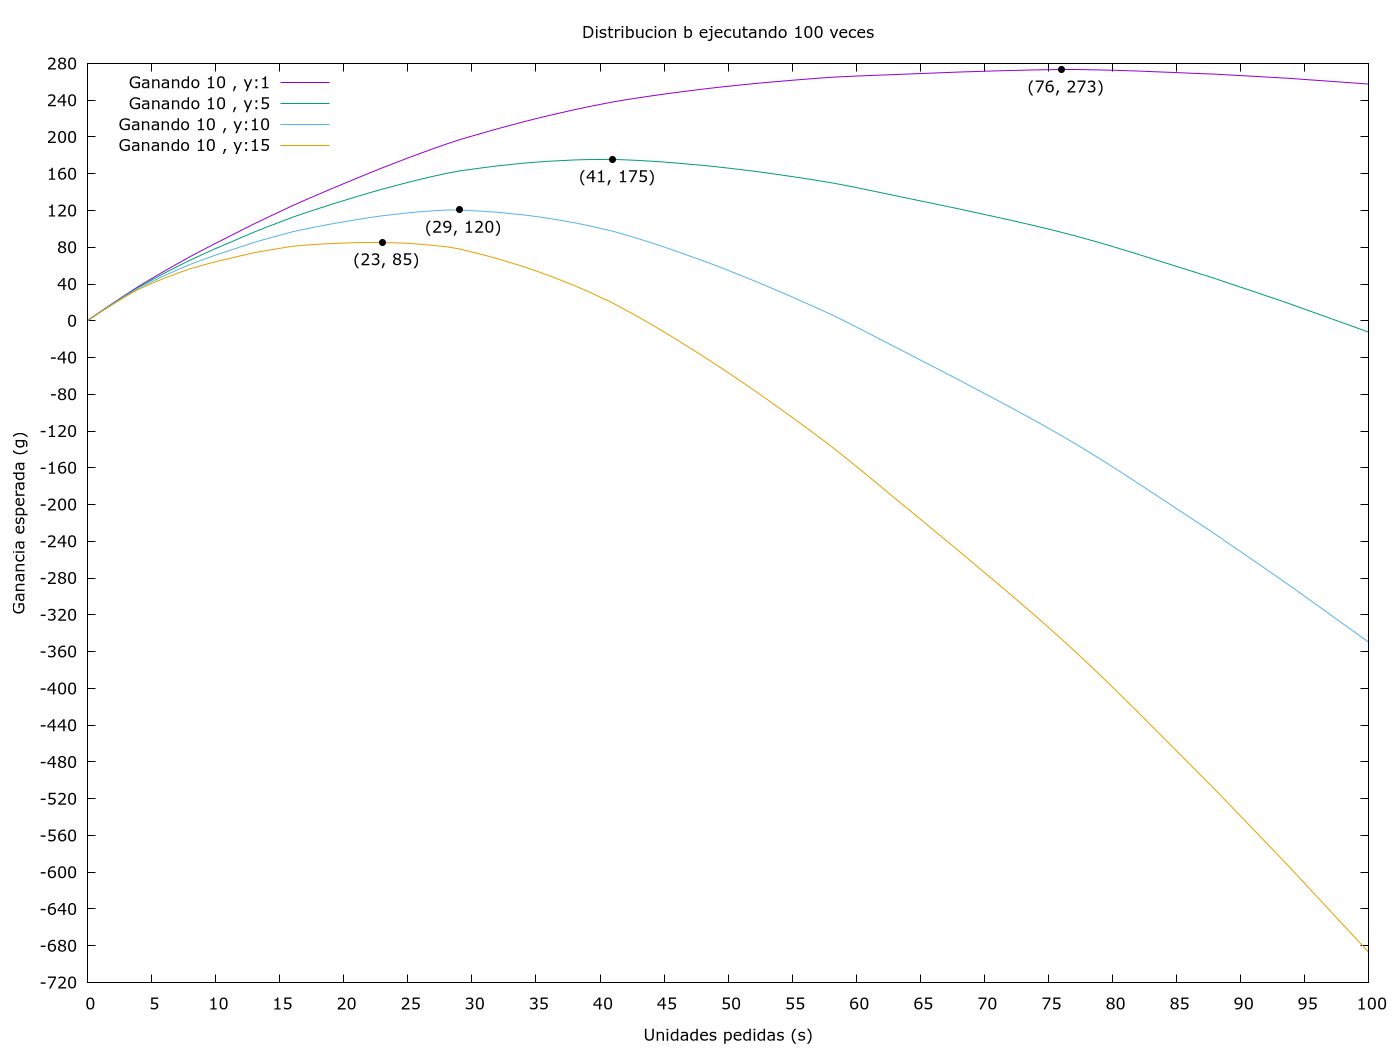
\includegraphics[scale = 0.2]{prob_b/datos_b_100.png}
	\caption{Con 100 repeticiones y la distribución b.}
	\label{fig:ej1_a_100}

\end{figure}

\begin{figure}[H]
	\centering
	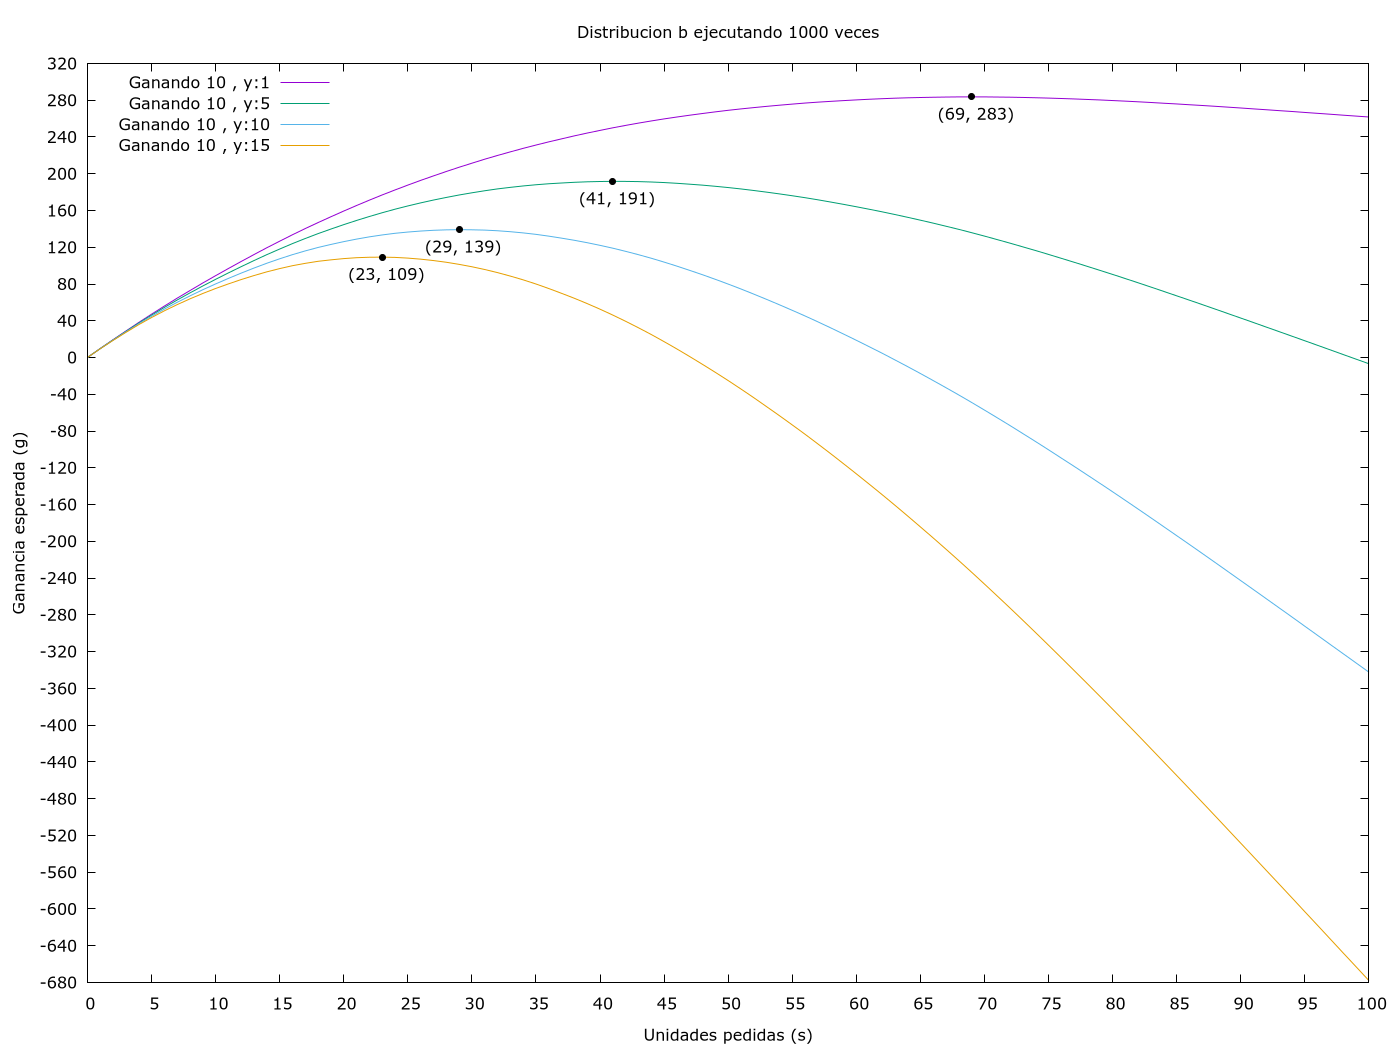
\includegraphics[scale = 0.2]{prob_b/datos_b_1000.png}
	\caption{Con 1000 repeticiones y la distribución b.}
	\label{fig:ej1_a_1000}

\end{figure}

\begin{figure}[H]
	\centering
	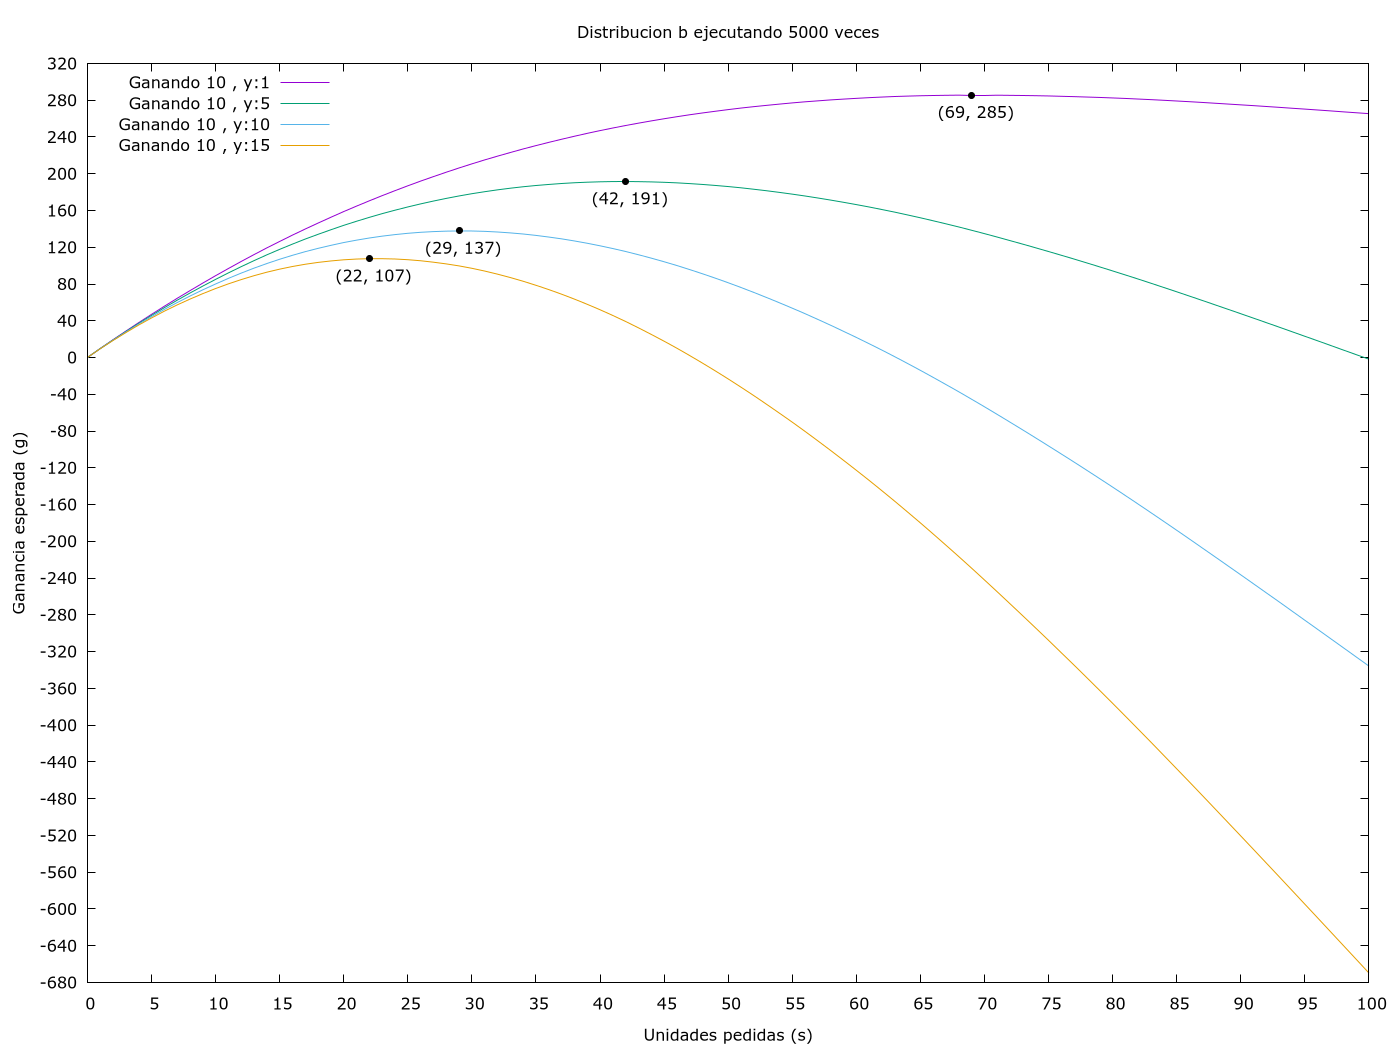
\includegraphics[scale = 0.2]{prob_b/datos_b_5000.png}
	\caption{Con 5000 repeticiones y la distribución b.}
	\label{fig:ej1_a_5000}

\end{figure}


\begin{figure}[H]
	\centering
	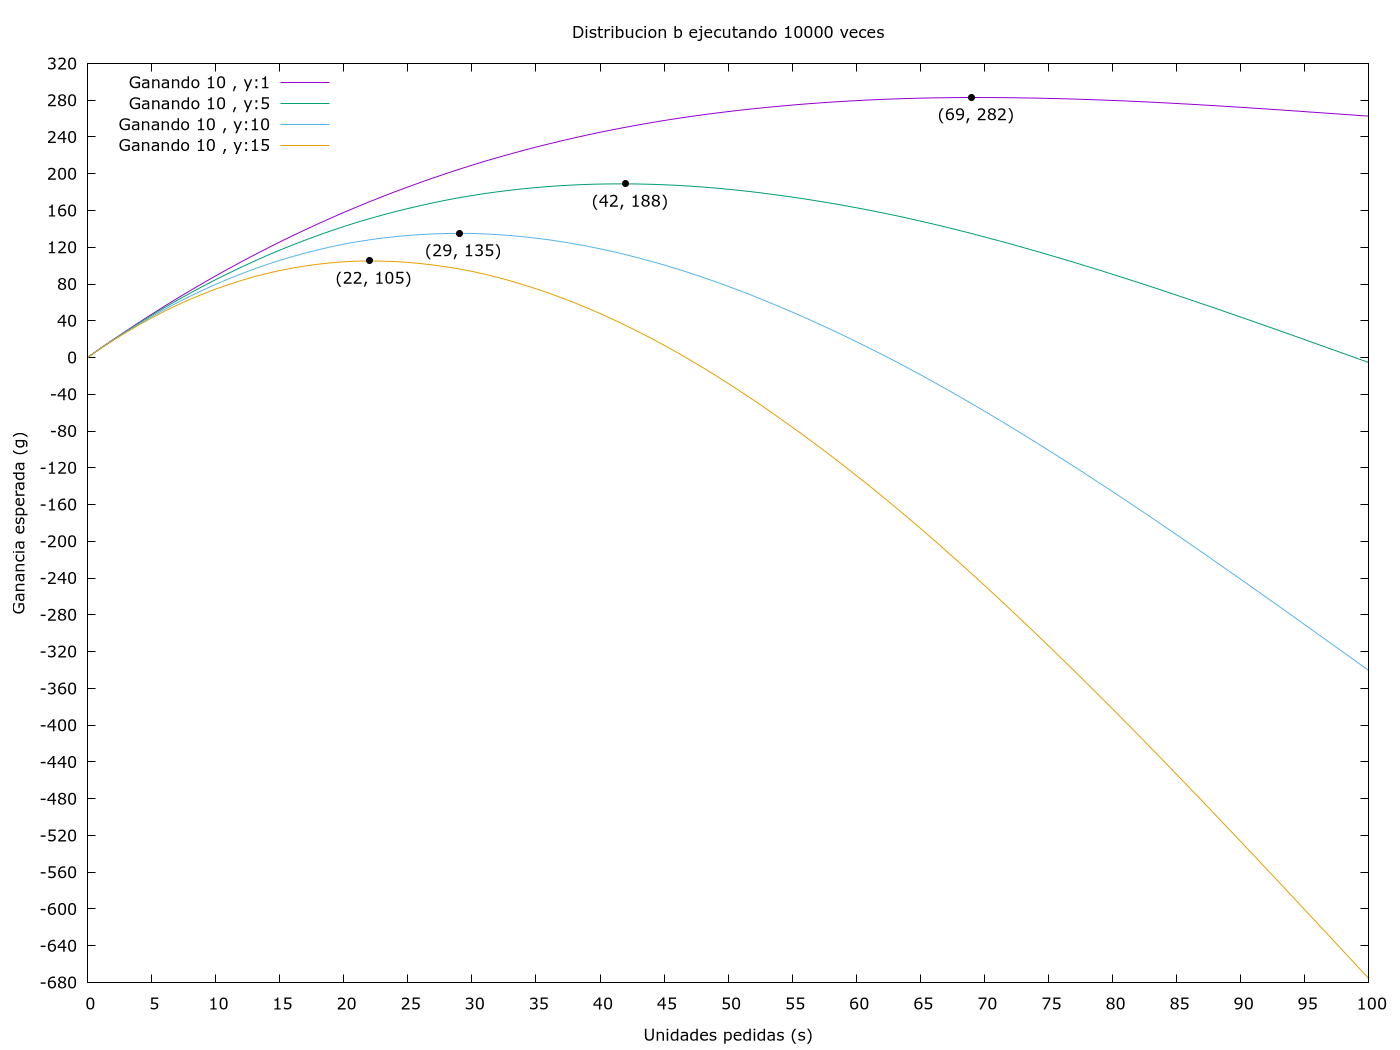
\includegraphics[scale = 0.2]{prob_b/datos_b_10000.png}
	\caption{Con 10000 repeticiones y la distribución b.}
	\label{fig:ej1_a_10000}

\end{figure}

\begin{figure}[H]
	\centering
	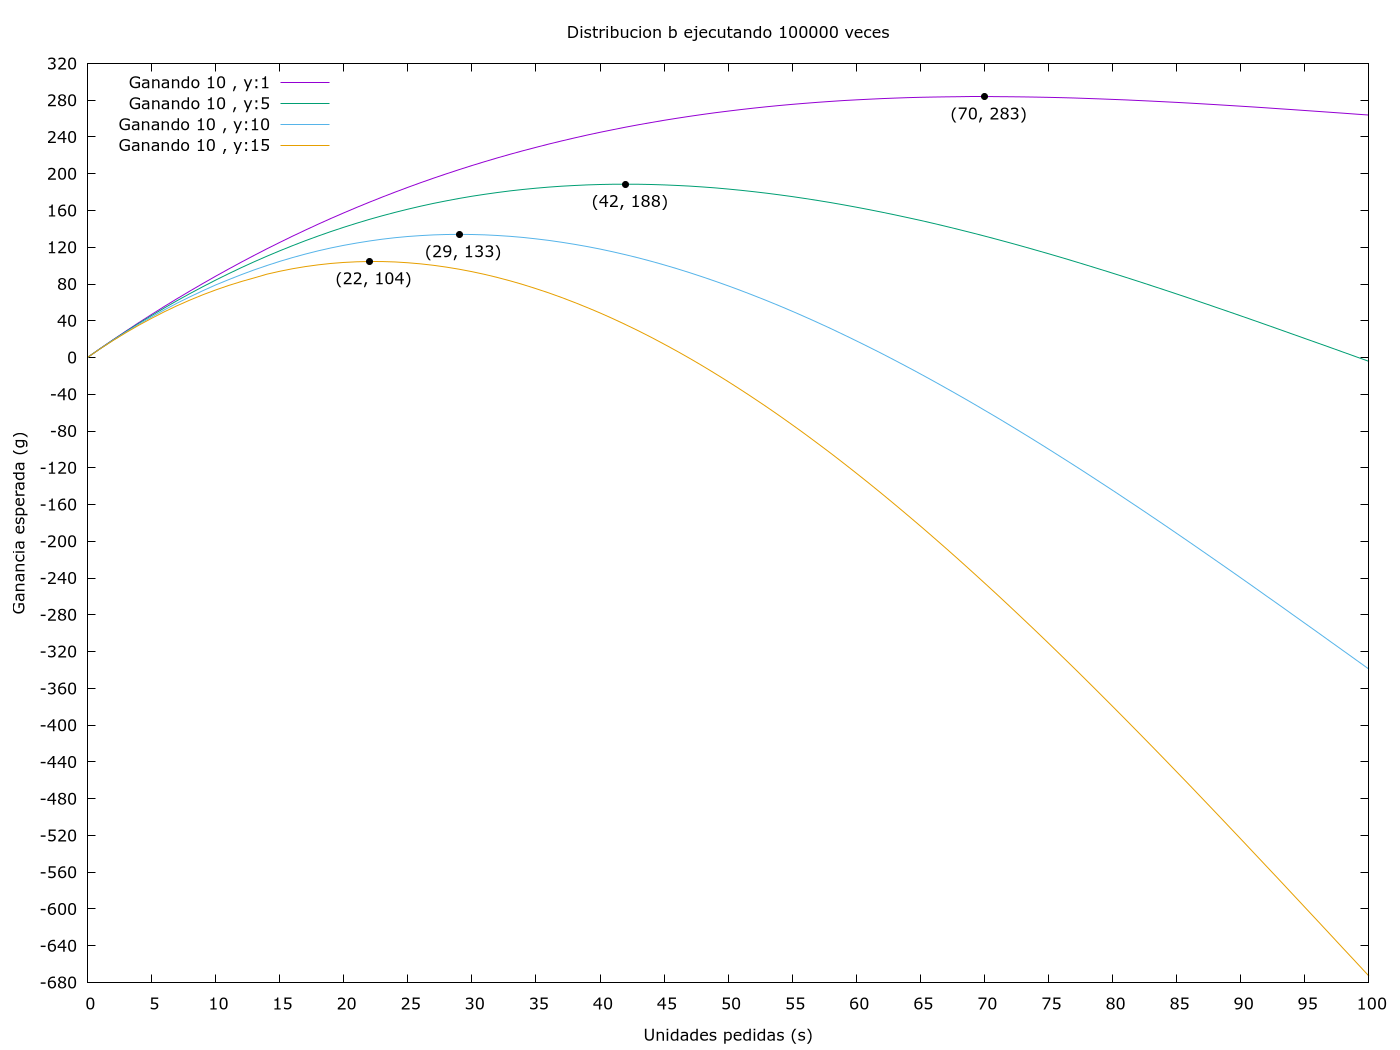
\includegraphics[scale = 0.2]{prob_b/datos_b_100000.png}
	\caption{Con 100000 repeticiones y la distribución b.}
	\label{fig:ej1_a_100000}

\end{figure}

\begin{figure}[H]
	\centering
	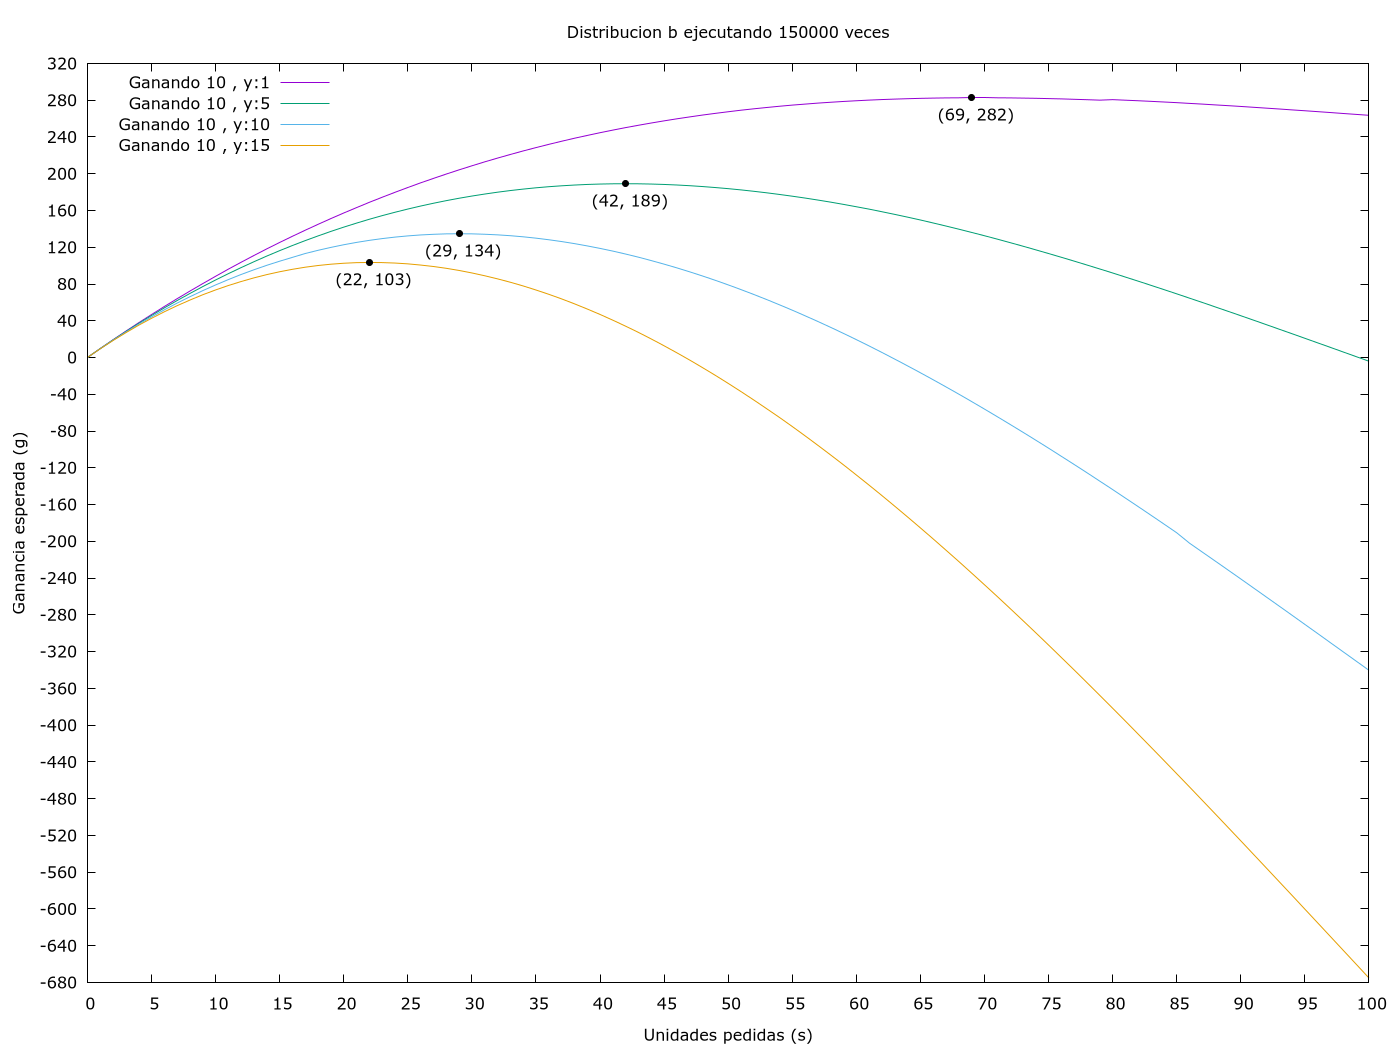
\includegraphics[scale = 0.2]{prob_b/datos_b_150000.png}
	\caption{Con 150000 repeticiones y la distribución b.}
	\label{fig:ej1_a_150000}

\end{figure}


Vemos como en este caso, en comparación con el caso a, los valores óptimos se encuentran mucho más a la izquierda en el eje X ya que es menos probable el que neceitemos una demanda alta, además de que las pérdidas son mucho mayores en valores altos, ya que casi nunca necesitaremos tantos periódicos, por lo que podemos intuir que el funcionamiento es correcto y se acerca a lo esperado.

Observamos que en el peor de los casos las pérdidas son mucho mayores que en el caso a, ya que es muy probable vender pocas unidades, por lo que si contratamos muchas, gran parte de estas no las conseguiremos vender, lo que supondrá un mayor coste.

En definitiva, si el modelo real sige esta probabilidad sería recomendable ser austero ya que un gran número de material contratado no sería viable venderlo en su mayoría.


\subsubsection{Resultados obtenidos con la distribución c}


La distribución c se basa en una distribución de probabilidad triangular, en la que los valores cercanos a 0 y 100 tienen la menor probabilidad a aparecer y los valores cercanos a 50 son más probables.

\begin{figure}[H]
	\centering
	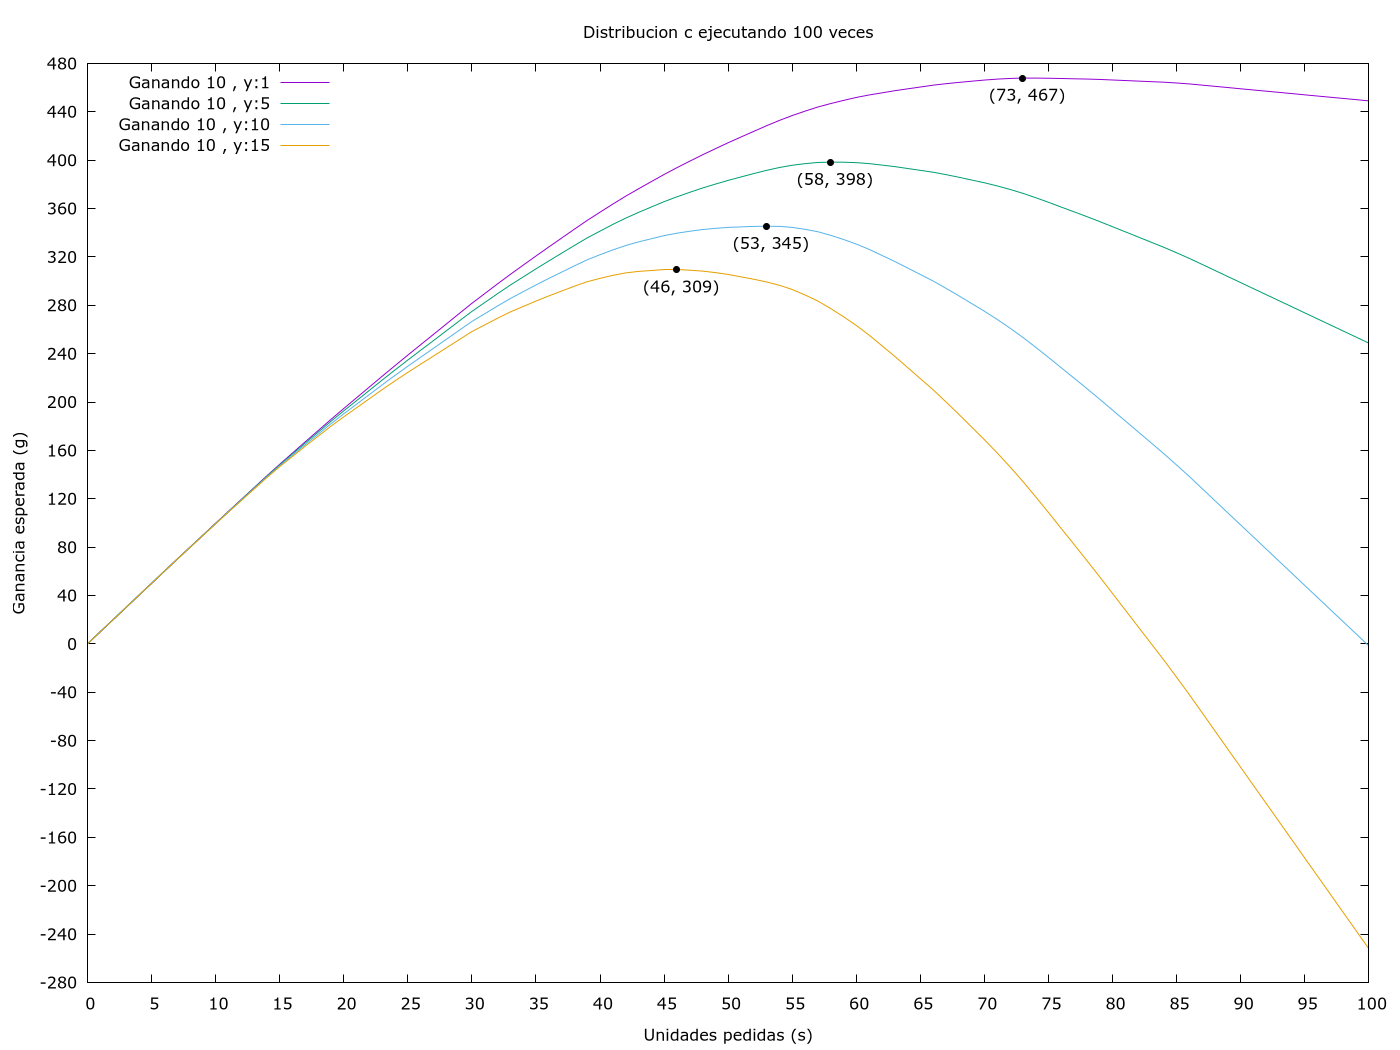
\includegraphics[scale = 0.2]{prob_c/datos_c_100.png}
	\caption{Con 100 repeticiones y la distribución c.}
	\label{fig:ej1_a_100}

\end{figure}

\begin{figure}[H]
	\centering
	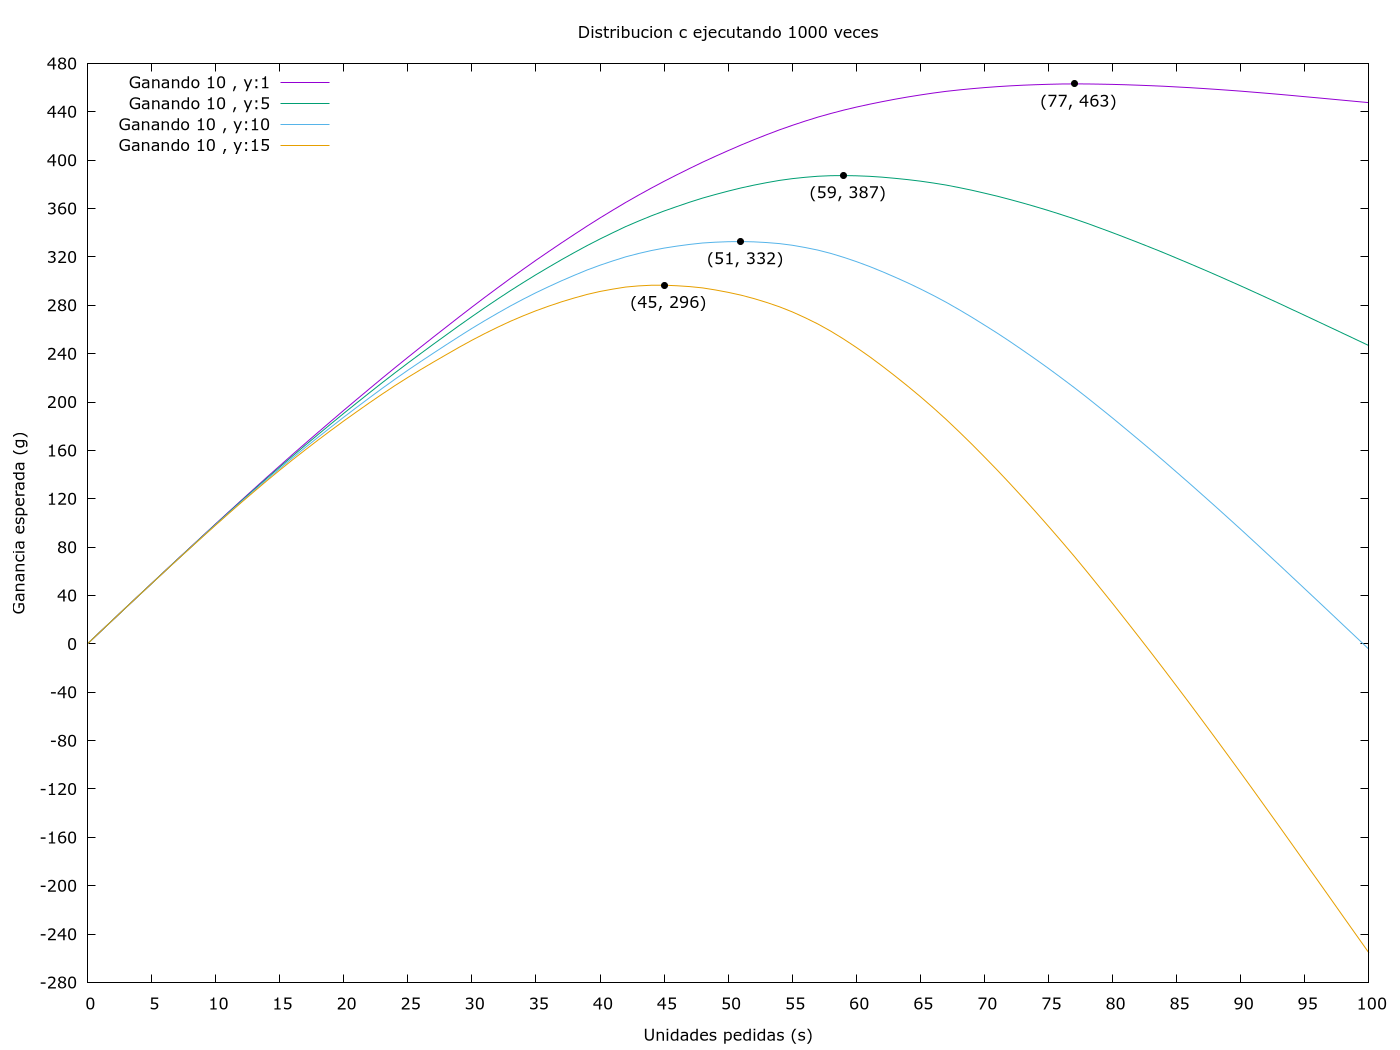
\includegraphics[scale = 0.2]{prob_c/datos_c_1000.png}
	\caption{Con 1000 repeticiones y la distribución c.}
	\label{fig:ej1_a_1000}

\end{figure}

\begin{figure}[H]
	\centering
	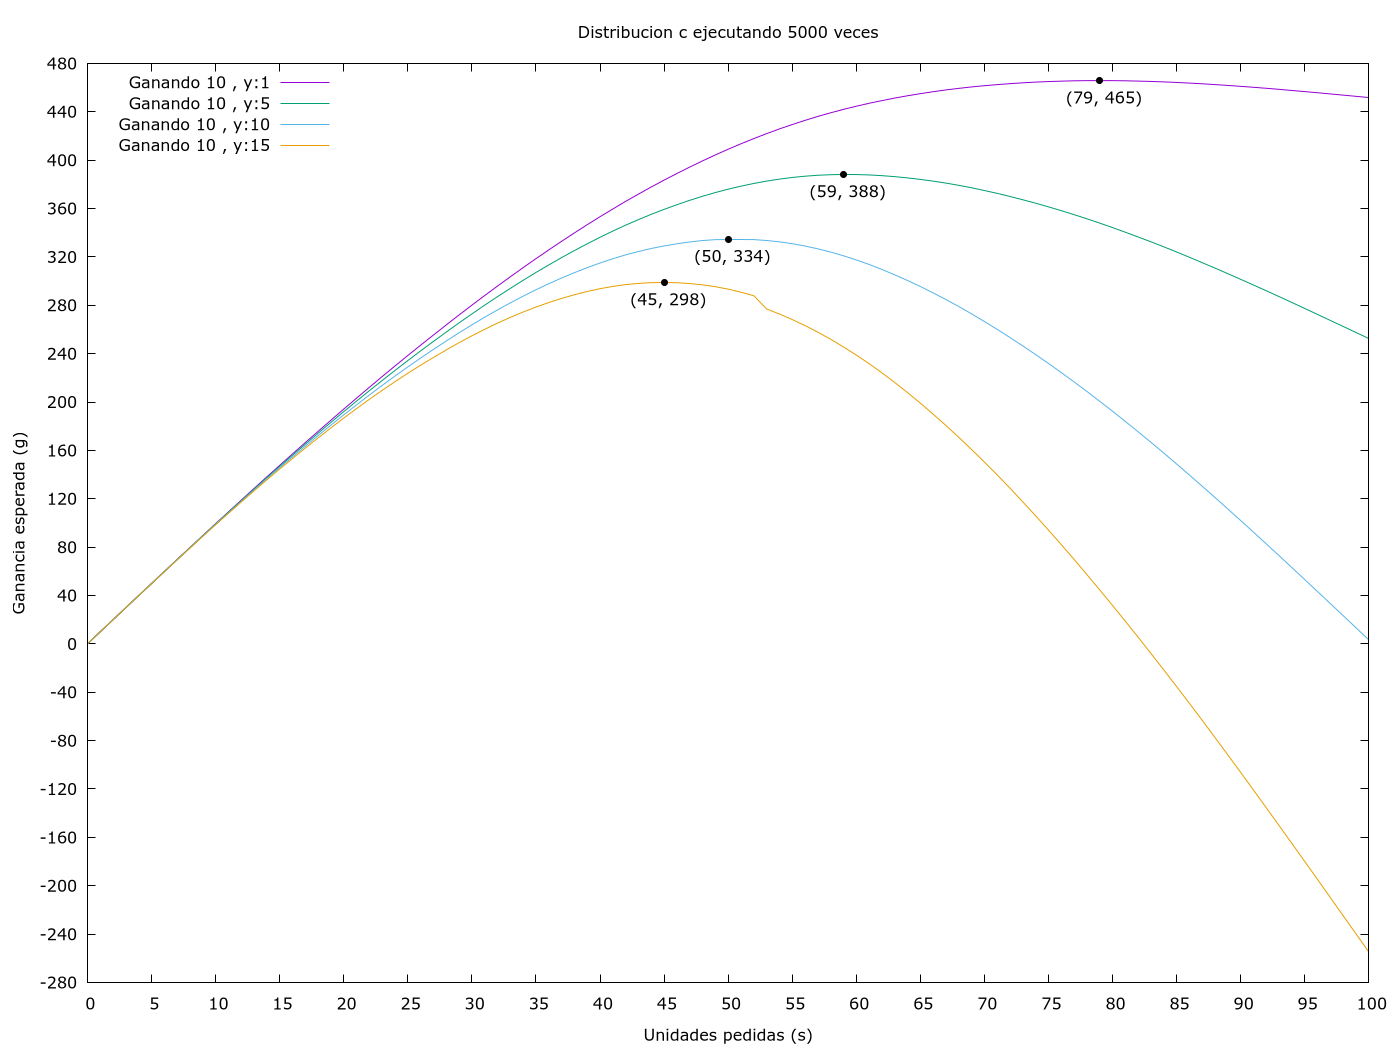
\includegraphics[scale = 0.2]{prob_c/datos_c_5000.png}
	\caption{Con 5000 repeticiones y la distribución c.}
	\label{fig:ej1_a_5000}

\end{figure}


\begin{figure}[H]
	\centering
	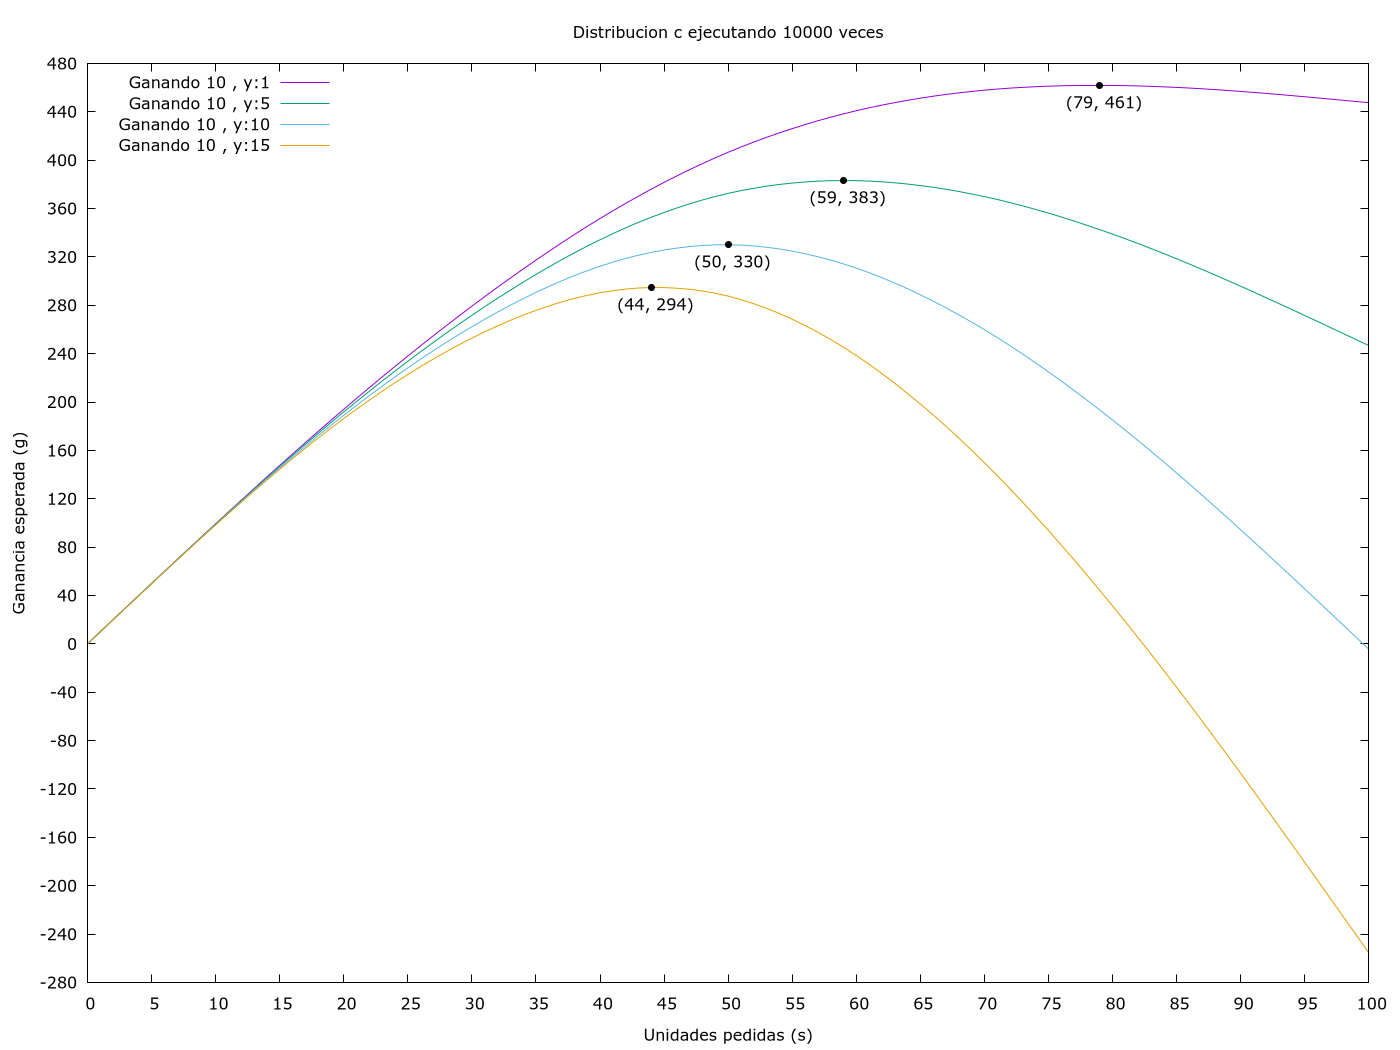
\includegraphics[scale = 0.2]{prob_c/datos_c_10000.png}
	\caption{Con 10000 repeticiones y la distribución c.}
	\label{fig:ej1_a_10000}

\end{figure}

\begin{figure}[H]
	\centering
	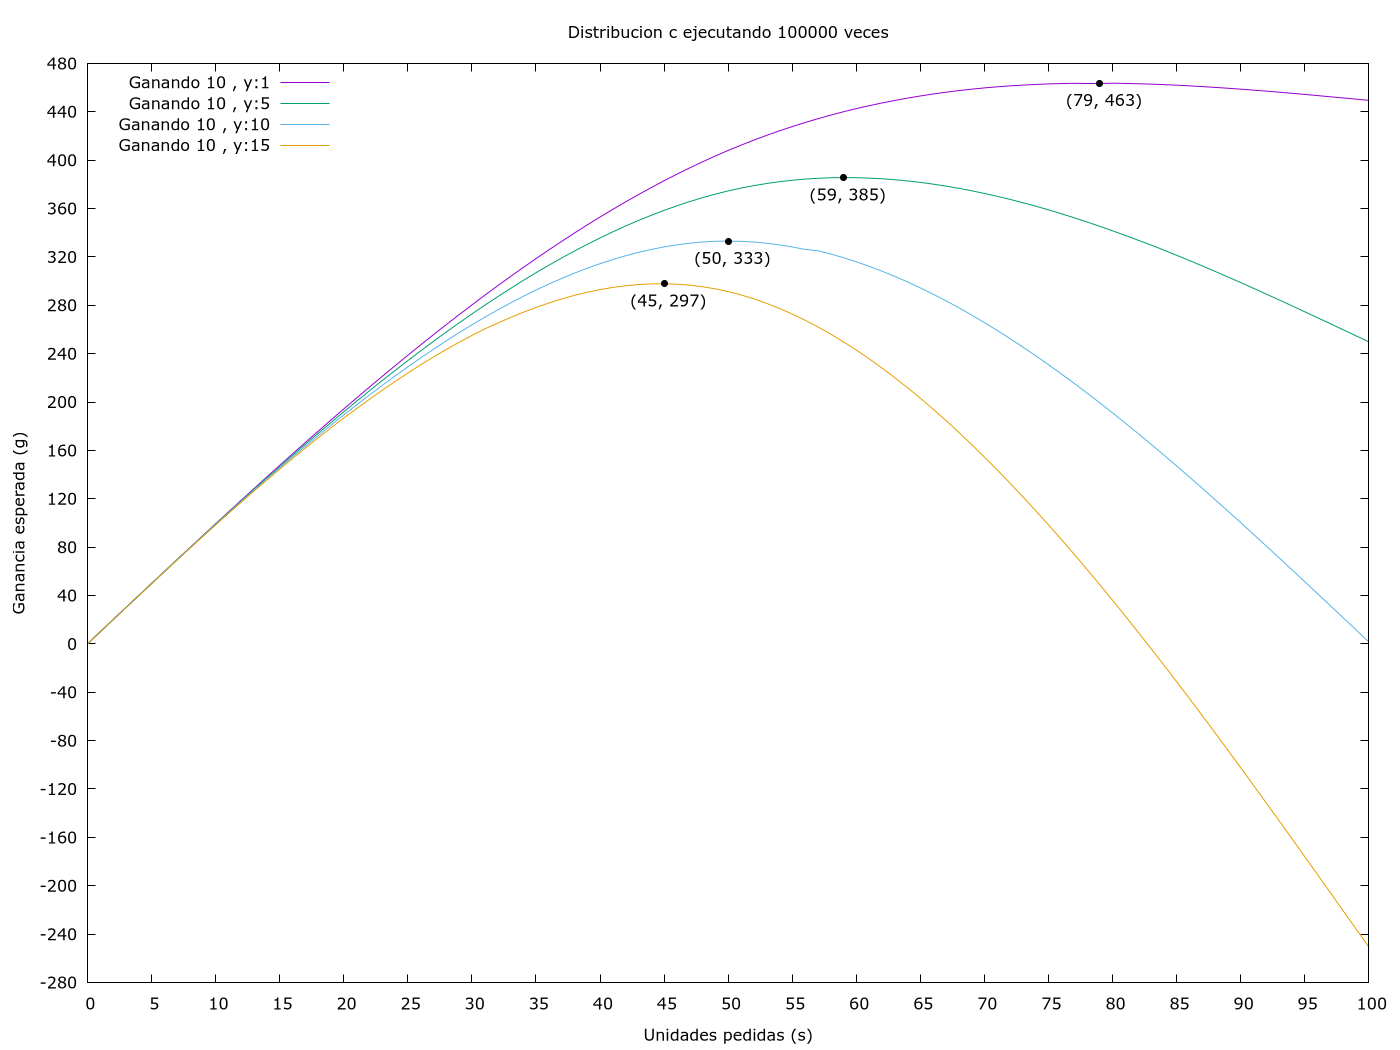
\includegraphics[scale = 0.2]{prob_c/datos_c_100000.png}
	\caption{Con 100000 repeticiones y la distribución c.}
	\label{fig:ej1_a_100000}

\end{figure}

\begin{figure}[H]
	\centering
	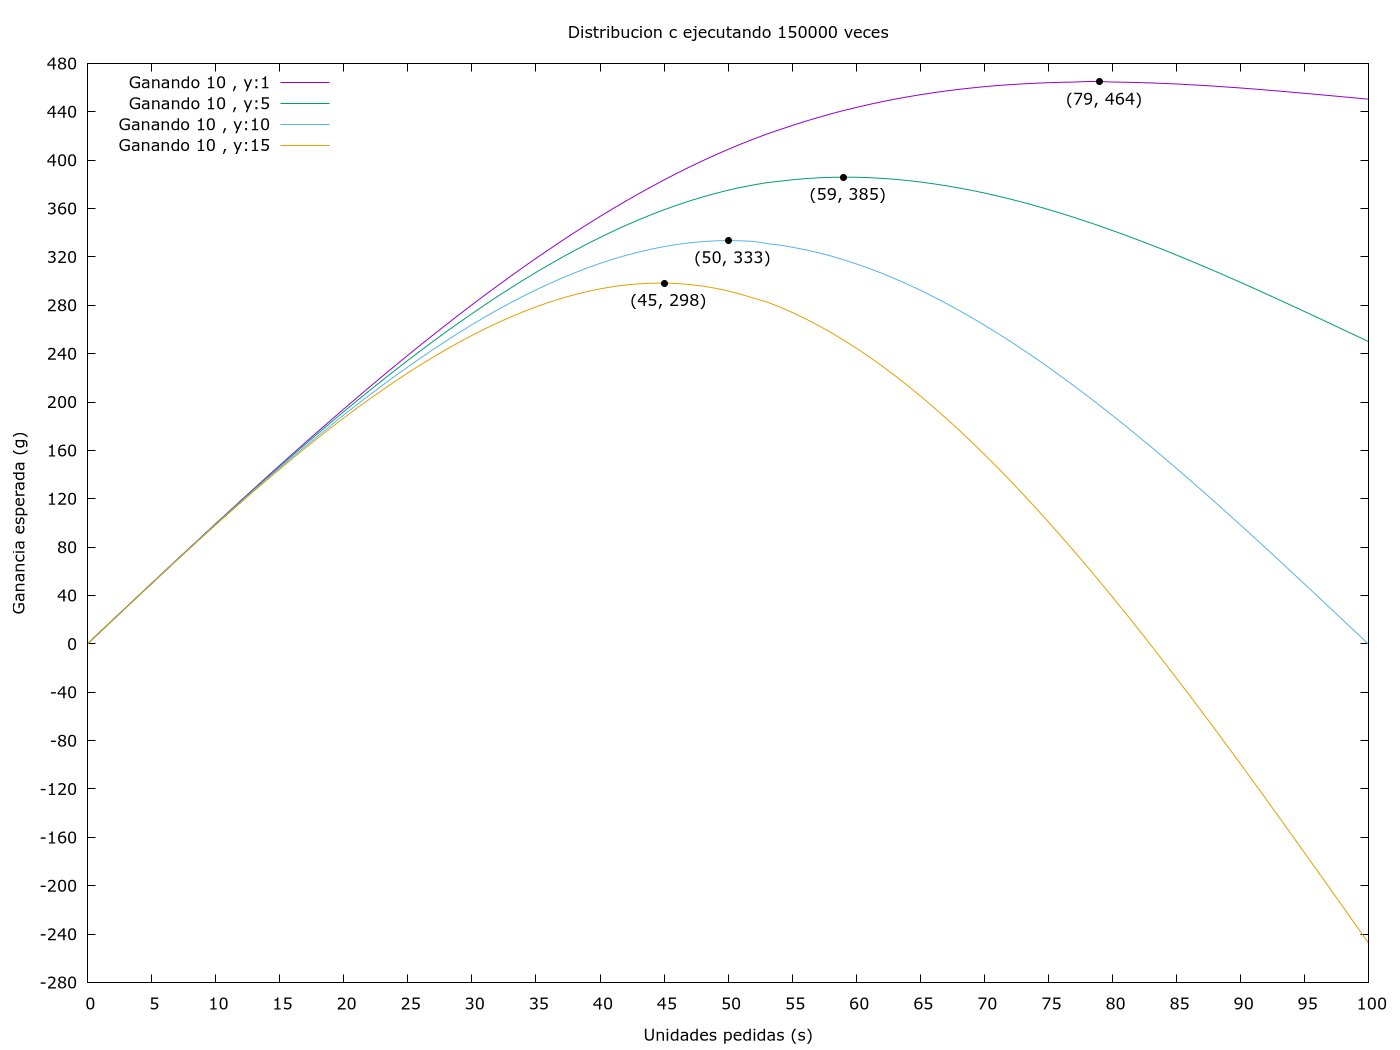
\includegraphics[scale = 0.2]{prob_c/datos_c_150000.png}
	\caption{Con 150000 repeticiones y la distribución c.}
	\label{fig:ej1_a_150000}

\end{figure}


En este caso vemos como al inicio en todos los casos la ganancia es similar, ya que es poco probable que se vendan pocos periódicos, haciendo que hasta los 25 periódicos aproximadamente la ganancia sea equivalente al venderlos siempre todos, llegano a alcanzar el máximo entre las 45 y 59 unidades en los distintos casos de penalización por periódico no vendido, hasta el óptimo en 79 si la penalización es muy baja.

Podemos ver que las perdidas que podemos llegar a alcanzar son similares a las del caso de la distribución a, porque en este caso es igual de probable que no se vendan ninguna unidad a muchas unidades, por lo que aunque contratemos una gran cantidad, se equilibra con las ventas, aunque en el caso extremo de unas pérdidas mayores que ganancias por periódico si nos generaría grandes pérdidas totales.

Si el modelo real sigue esta distribución sería el caso más favorable si la penalización por no vender un periódico es muy grande, ya que nos aseguraríamos que una cantidad sustancial de periódicos vendidos. Sin embargo, en casos en los que la penalización no es tan grande, la distribución a nos ofrece buenos resultados.

\subsection{Modificación 1 del modelo}

Tras la experimentación anterior se nos pide incluir un nuevo modelo de funcionamiento en nuestro modelo, en el que en lugar de tener un gasto por cada unidad no vendida, se cobrará un único gasto fijo $z$ como devolución, por lo que si vendemos todas las unidades no se pagará nada, pero si no se vende alguna unidad, indiferentemente del número de unidades sin vender, se pagarán $z$ euros por la devolución.

Estudiaremos esta modificación con unos valores de $z = 10, 50, 100, 500$ y para las tres distribuciones de probabilidad.

\subsubsection{Resultados obtenidos con la distribución a}


\begin{figure}[H]
	\centering
	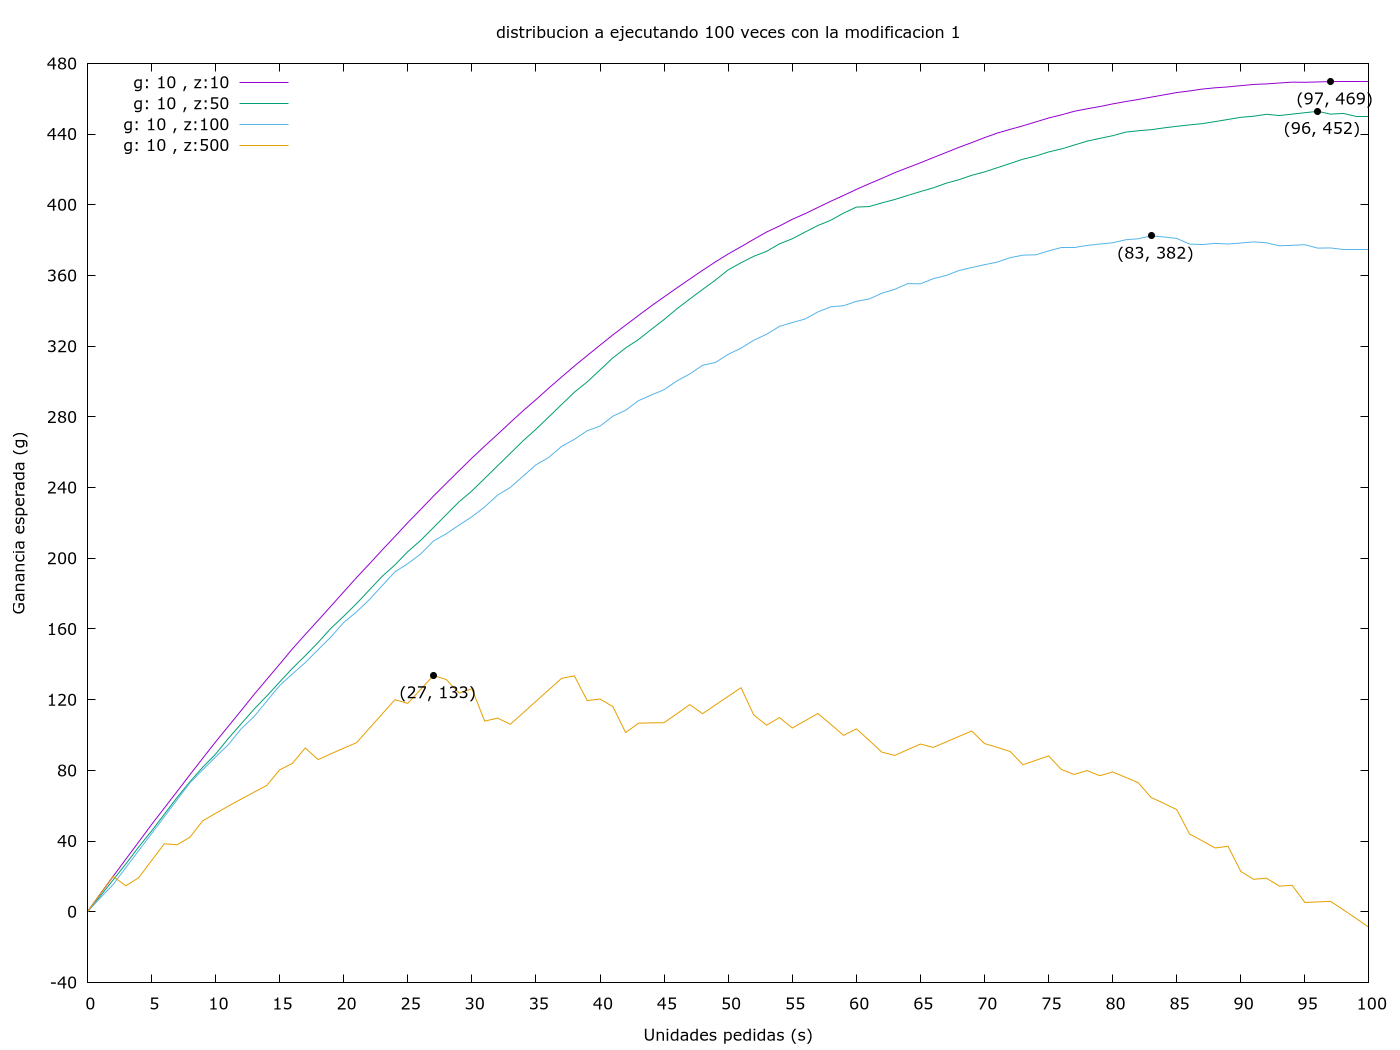
\includegraphics[scale = 0.2]{prob_a/datos_a_100_1.png}
	\caption{Con 100 repeticiones, la distribución a y la modificación 1.}
	\label{fig:ej1_a_100}

\end{figure}

\begin{figure}[H]
	\centering
	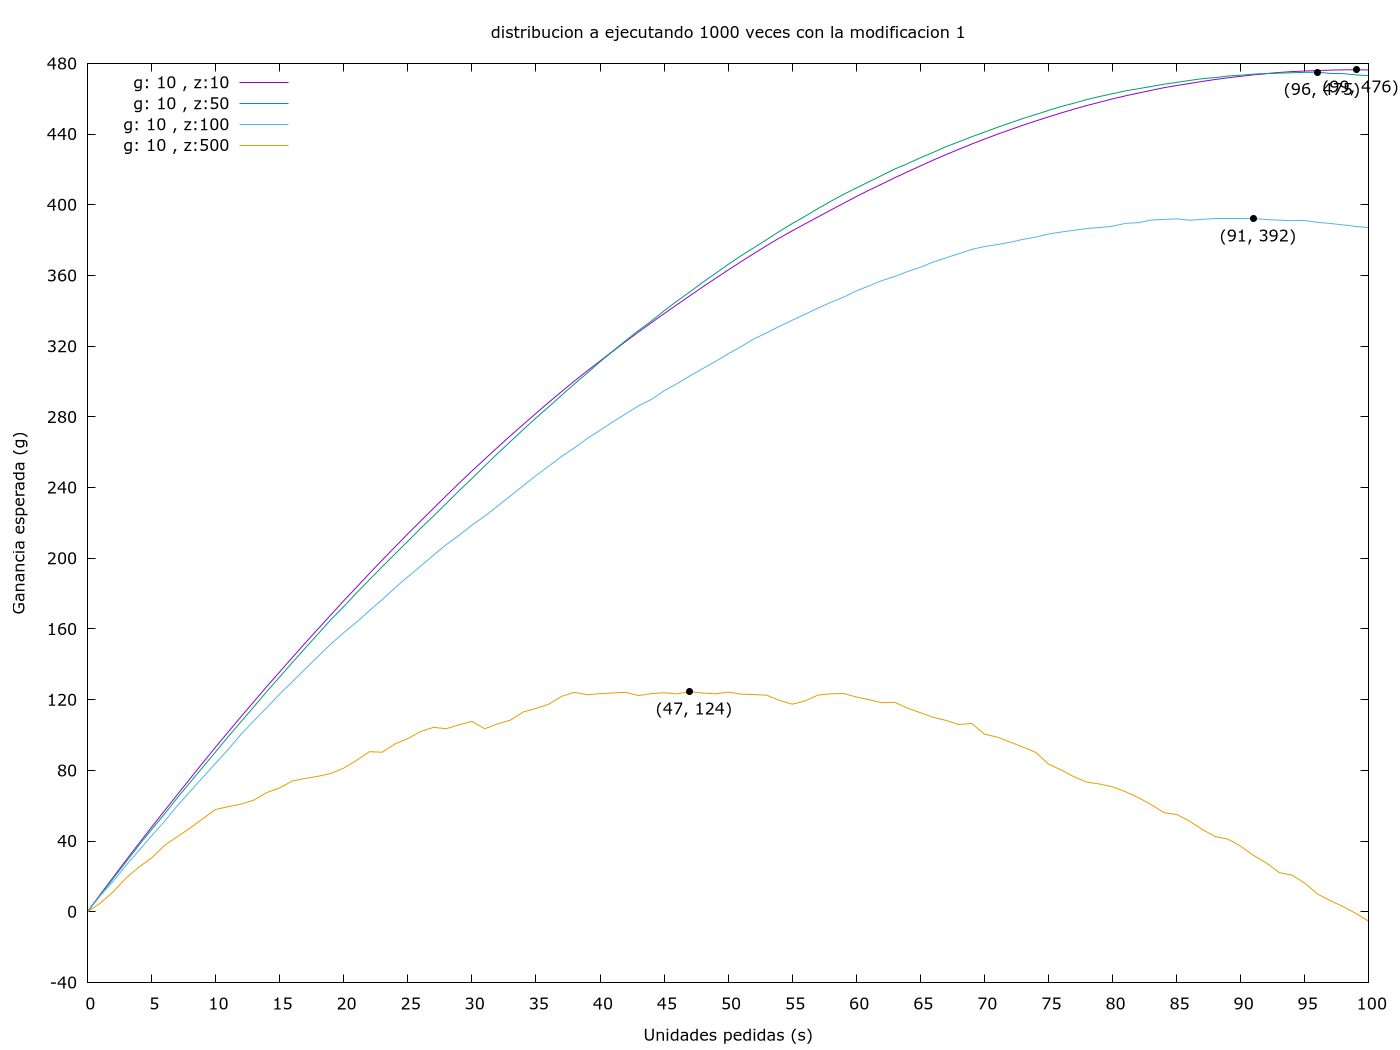
\includegraphics[scale = 0.2]{prob_a/datos_a_1000_1.png}
	\caption{Con 1000 repeticiones, la distribución a y la modificación 1.}
	\label{fig:ej1_a_1000}

\end{figure}

\begin{figure}[H]
	\centering
	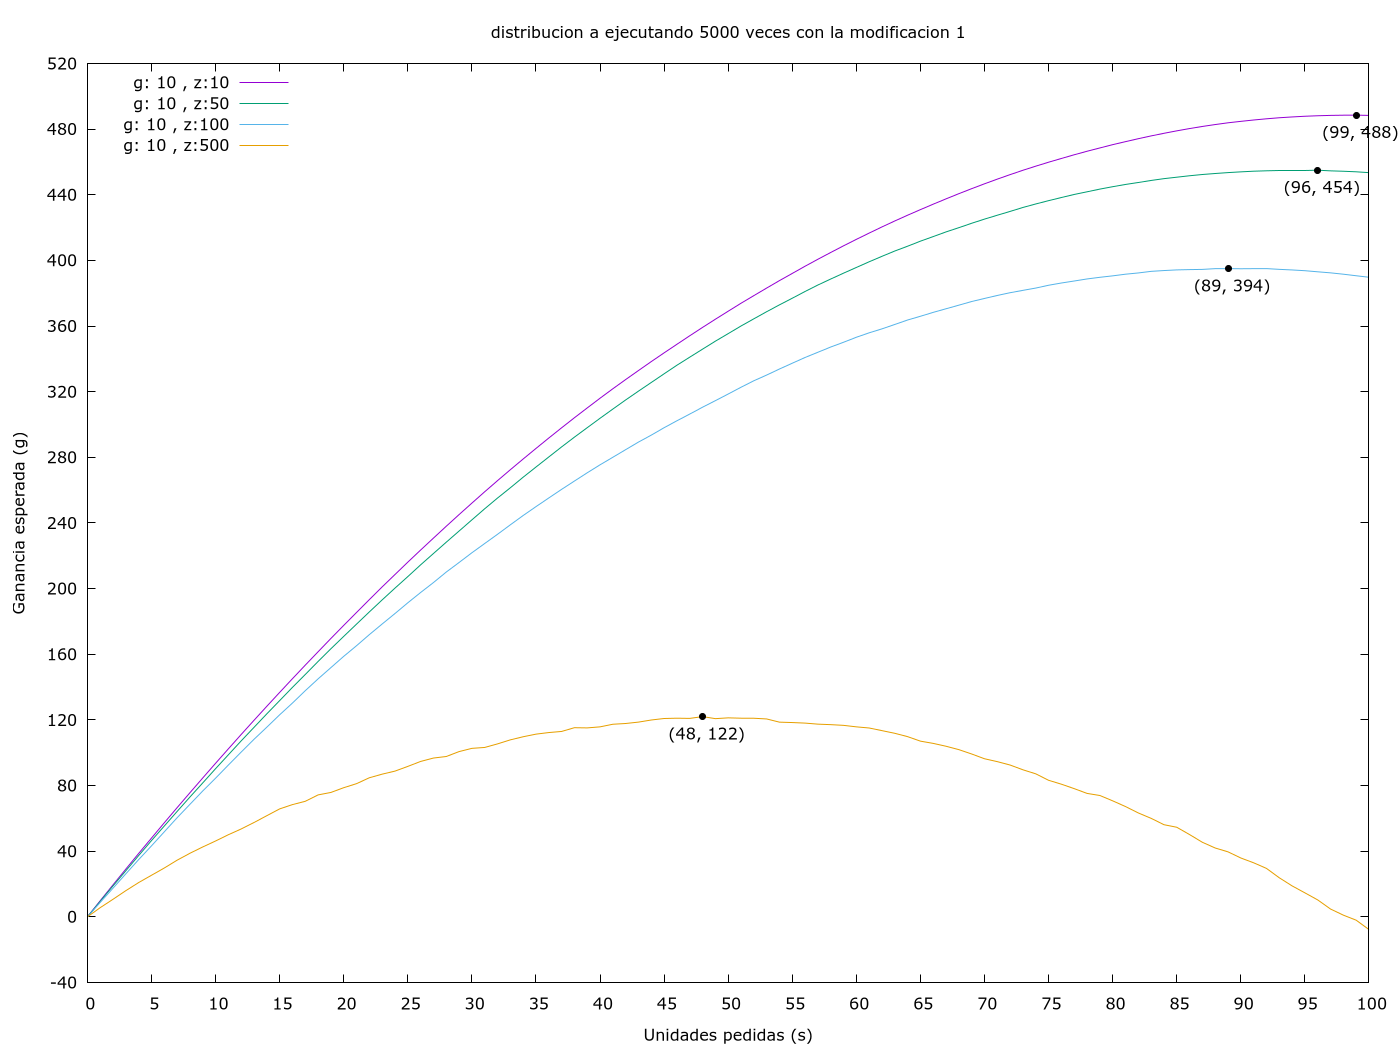
\includegraphics[scale = 0.2]{prob_a/datos_a_5000_1.png}
	\caption{Con 5000 repeticiones, la distribución a y la modificación 1.}
	\label{fig:ej1_a_5000}

\end{figure}


\begin{figure}[H]
	\centering
	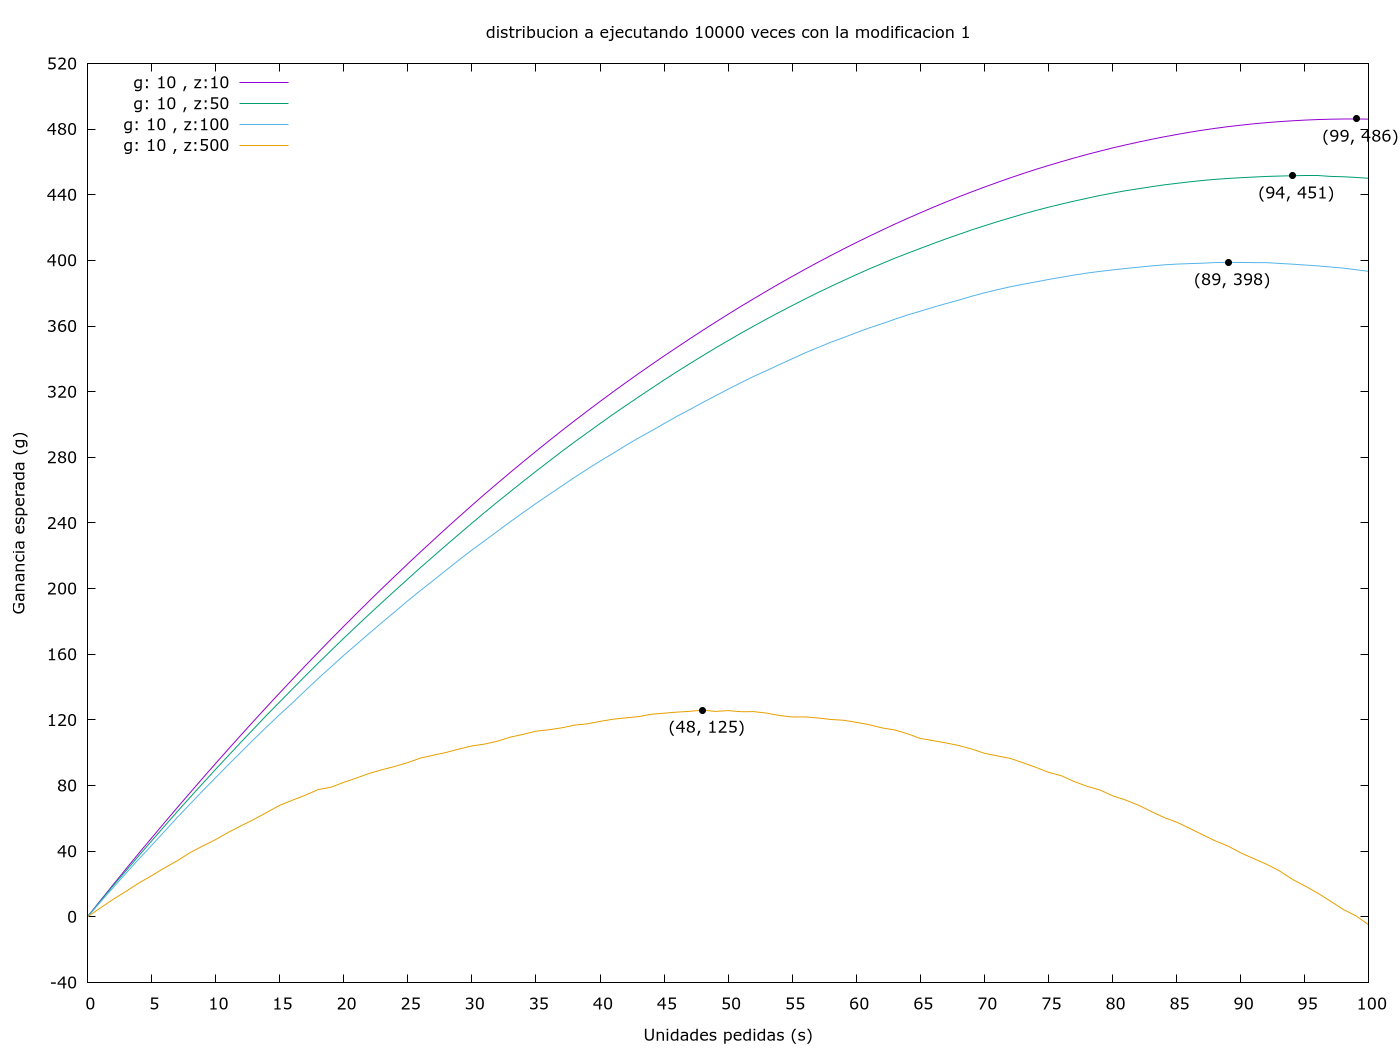
\includegraphics[scale = 0.2]{prob_a/datos_a_10000_1.png}
	\caption{Con 10000 repeticiones, la distribución a y la modificación 1.}
	\label{fig:ej1_a_10000}

\end{figure}

\begin{figure}[H]
	\centering
	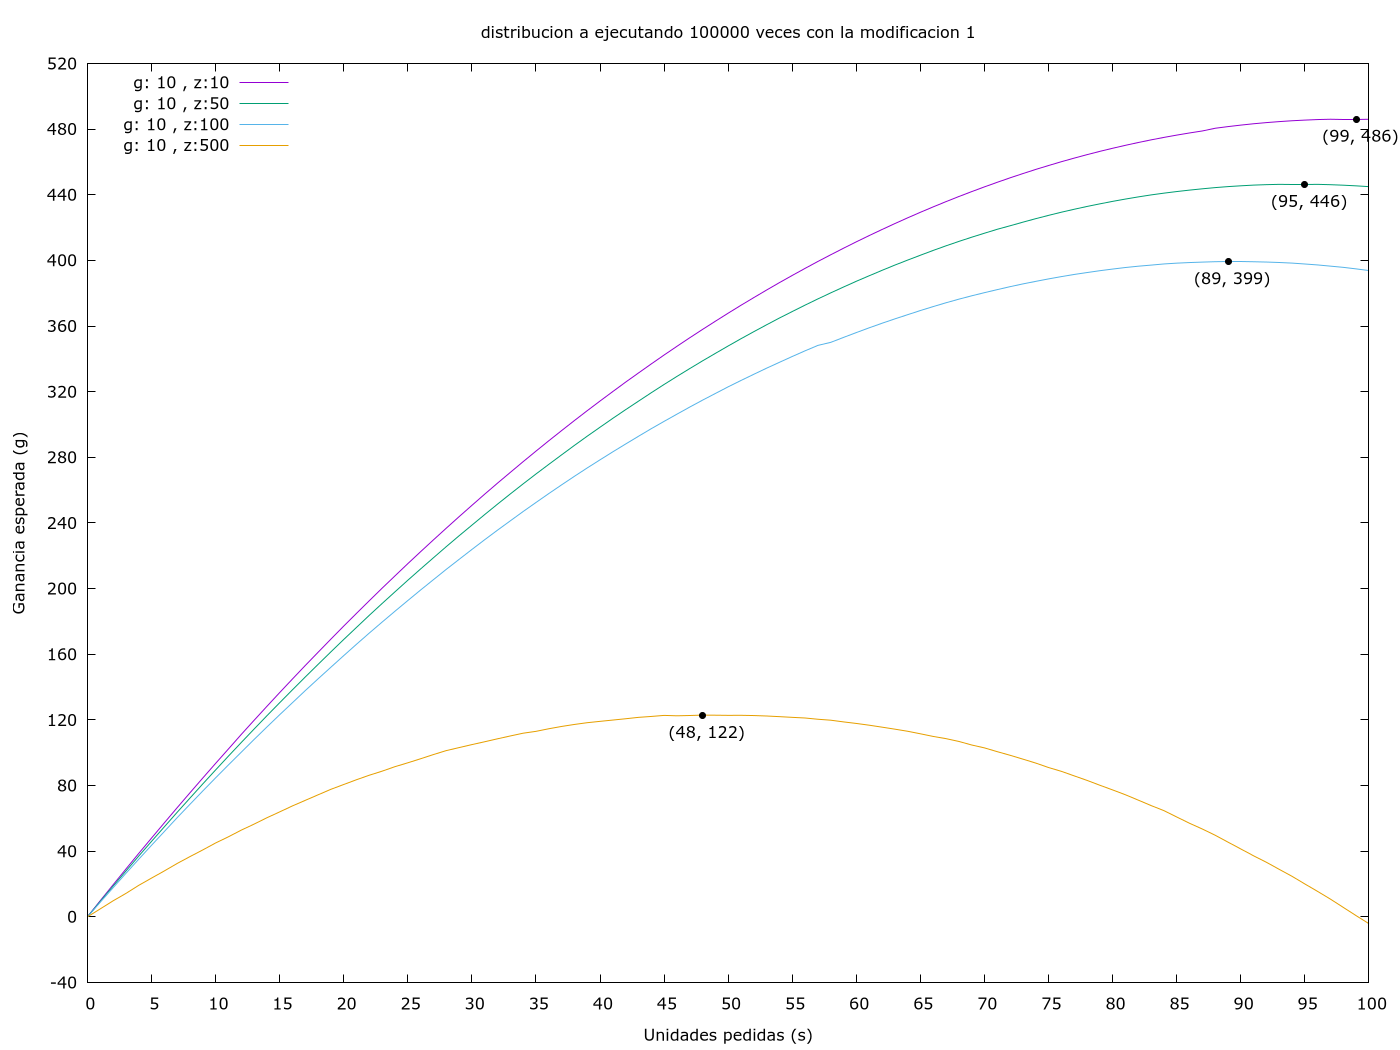
\includegraphics[scale = 0.2]{prob_a/datos_a_100000_1.png}
	\caption{Con 100000 repeticiones, la distribución a y la modificación 1.}
	\label{fig:ej1_a_100000}

\end{figure}

\begin{figure}[H]
	\centering
	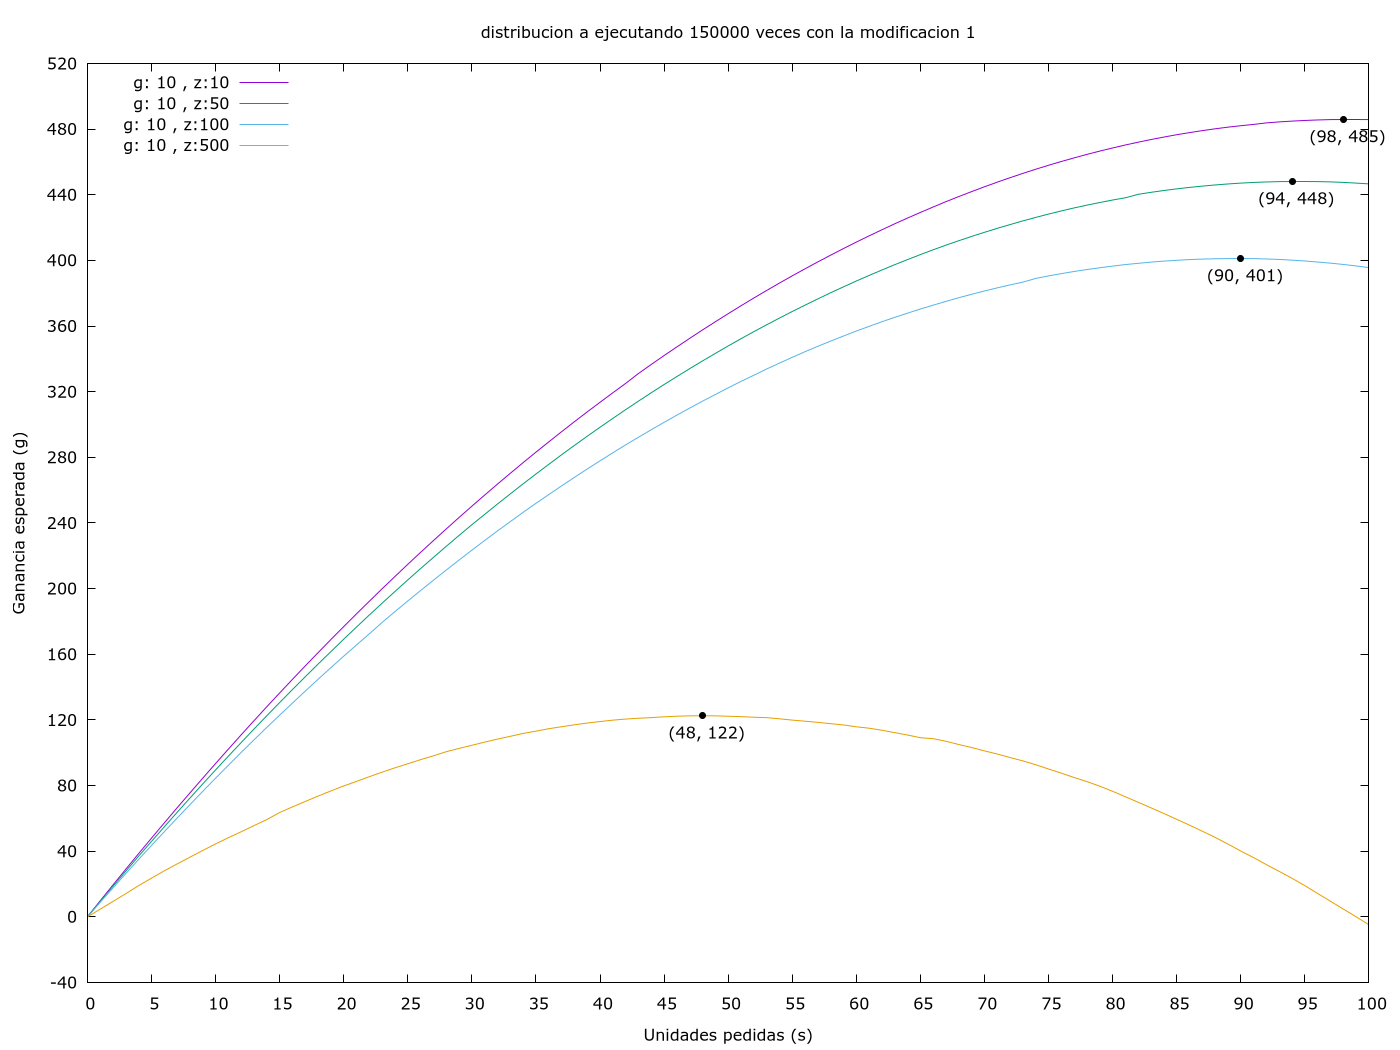
\includegraphics[scale = 0.2]{prob_a/datos_a_150000_1.png}
	\caption{Con 150000 repeticiones, la distribución a y la modificación 1.}
	\label{fig:ej1_a_150000}

\end{figure}


Vemos como en las ejecuciones con pocas repeticiones la curva se hace más dificil de interpretar, por lo que de nuevo me centraré en las ejecuciones con más repeticiones.

Obervamos como en este caso la caida de las curvas es mucho más suave, haciendo que solo tengamos un caso de perdidas si el precio de la devolución es de 500 euros.

En este caso, podemos ver que claramente la ganancia es mayor que sin la modificación, ya que cuando no se llega a vender una unidad, es indiferente el número de unidades no vendidas.



\subsubsection{Resultados obtenidos con la distribución b}



\begin{figure}[H]
	\centering
	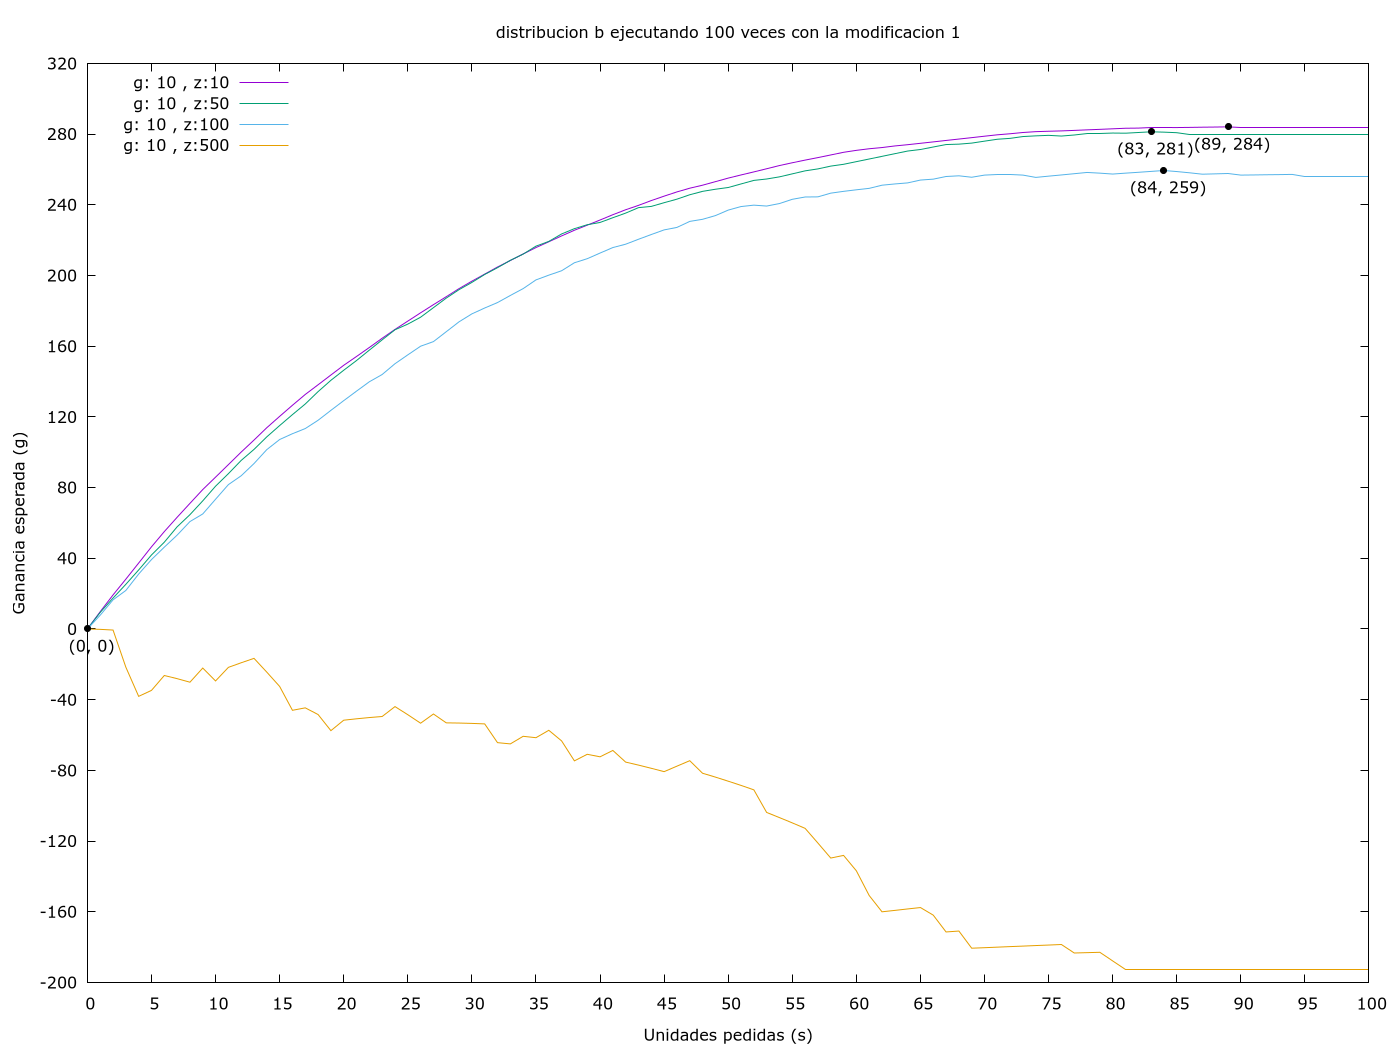
\includegraphics[scale = 0.2]{prob_b/datos_b_100_1.png}
	\caption{Con 100 repeticiones, la distribución b y la modificación 1.}
	\label{fig:ej1_a_100}

\end{figure}

\begin{figure}[H]
	\centering
	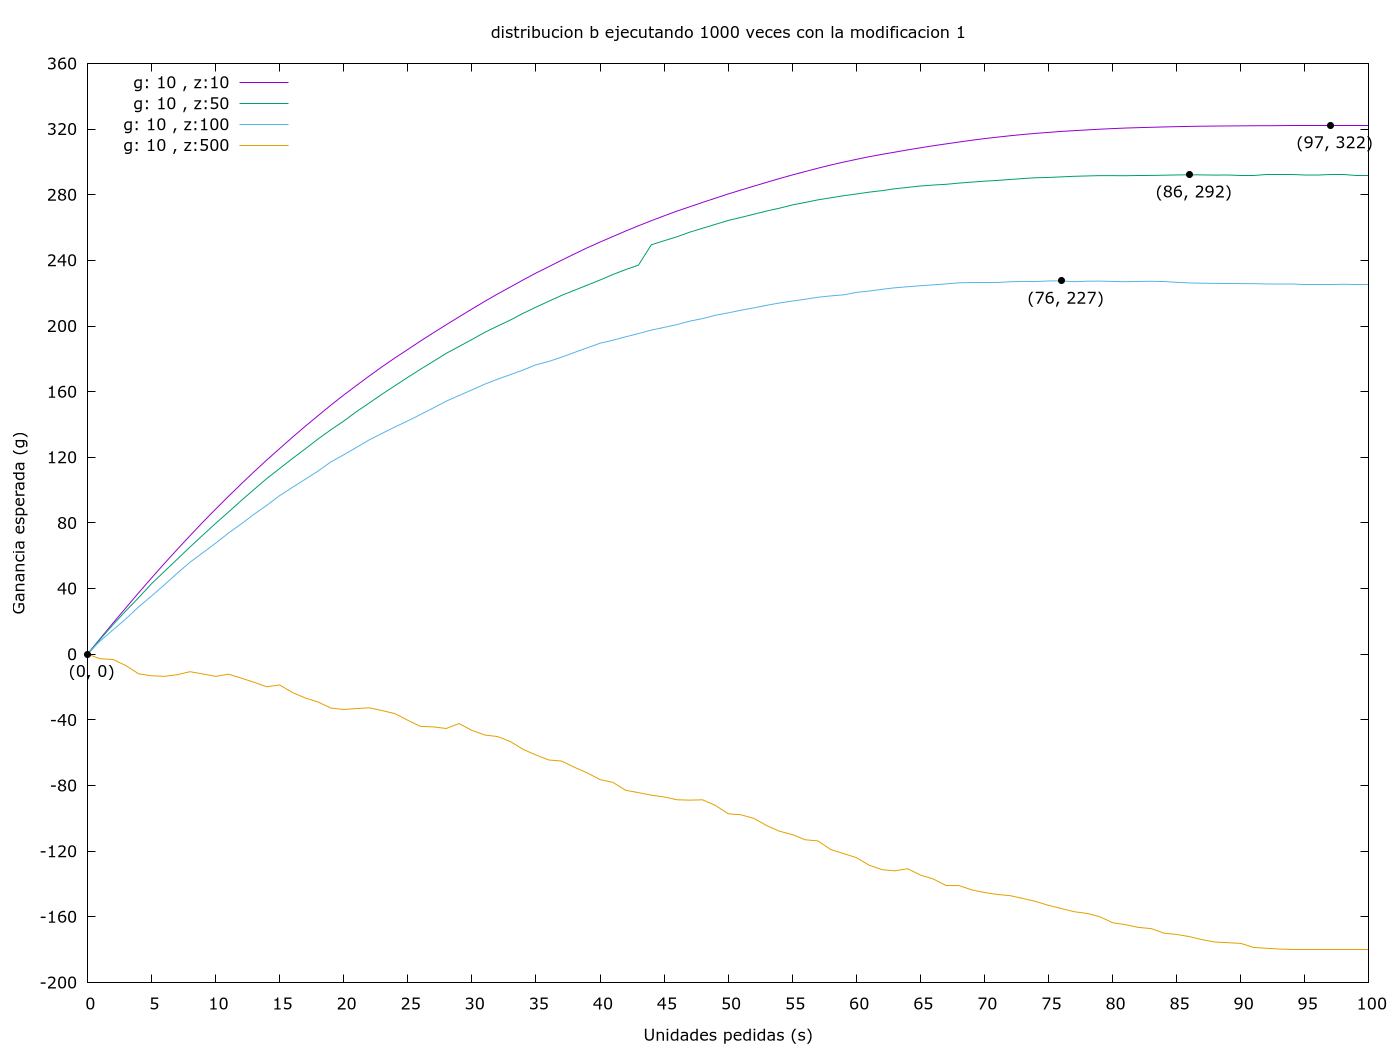
\includegraphics[scale = 0.2]{prob_b/datos_b_1000_1.png}
	\caption{Con 1000 repeticiones, la distribución b y la modificación 1.}
	\label{fig:ej1_a_1000}

\end{figure}

\begin{figure}[H]
	\centering
	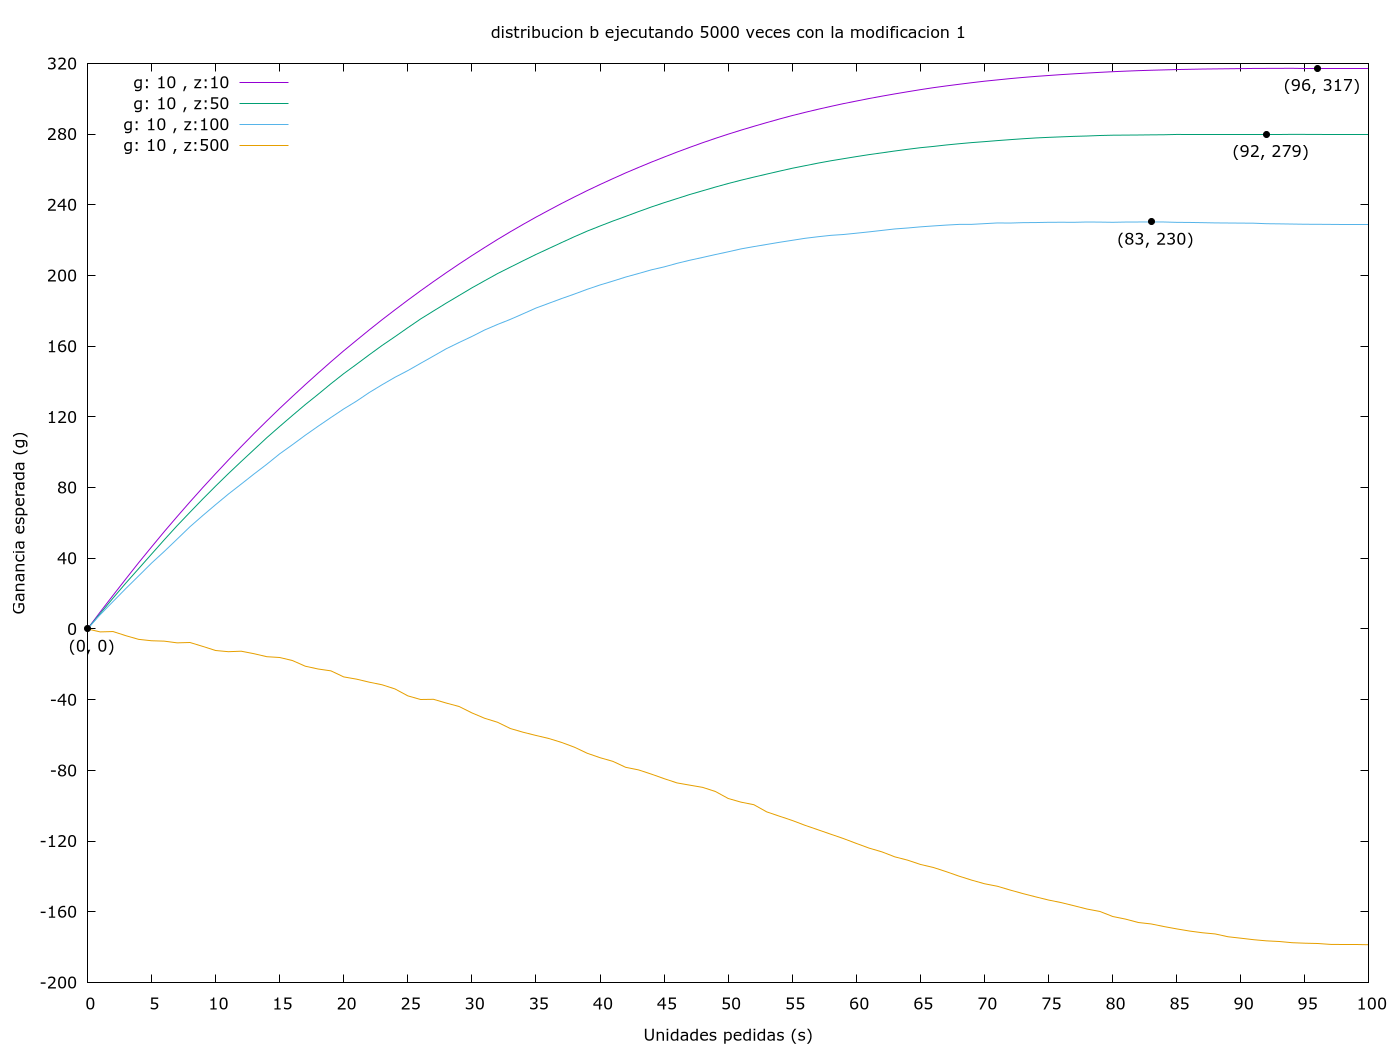
\includegraphics[scale = 0.2]{prob_b/datos_b_5000_1.png}
	\caption{Con 5000 repeticiones, la distribución b y la modificación 1.}
	\label{fig:ej1_a_5000}

\end{figure}


\begin{figure}[H]
	\centering
	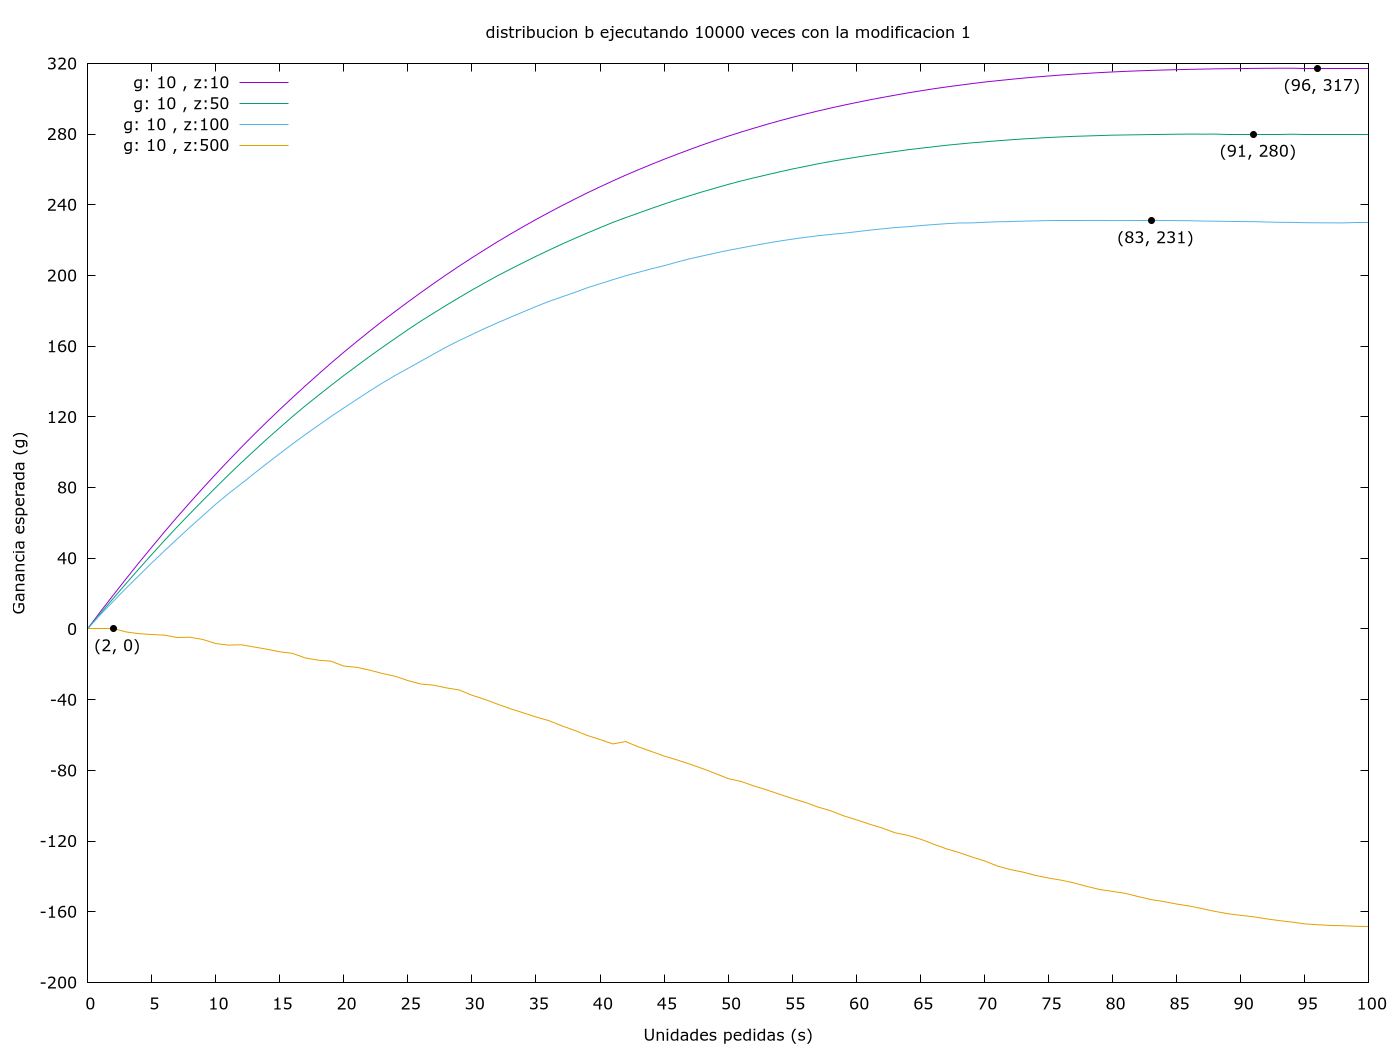
\includegraphics[scale = 0.2]{prob_b/datos_b_10000_1.png}
	\caption{Con 10000 repeticiones, la distribución b y la modificación 1.}
	\label{fig:ej1_a_10000}

\end{figure}

\begin{figure}[H]
	\centering
	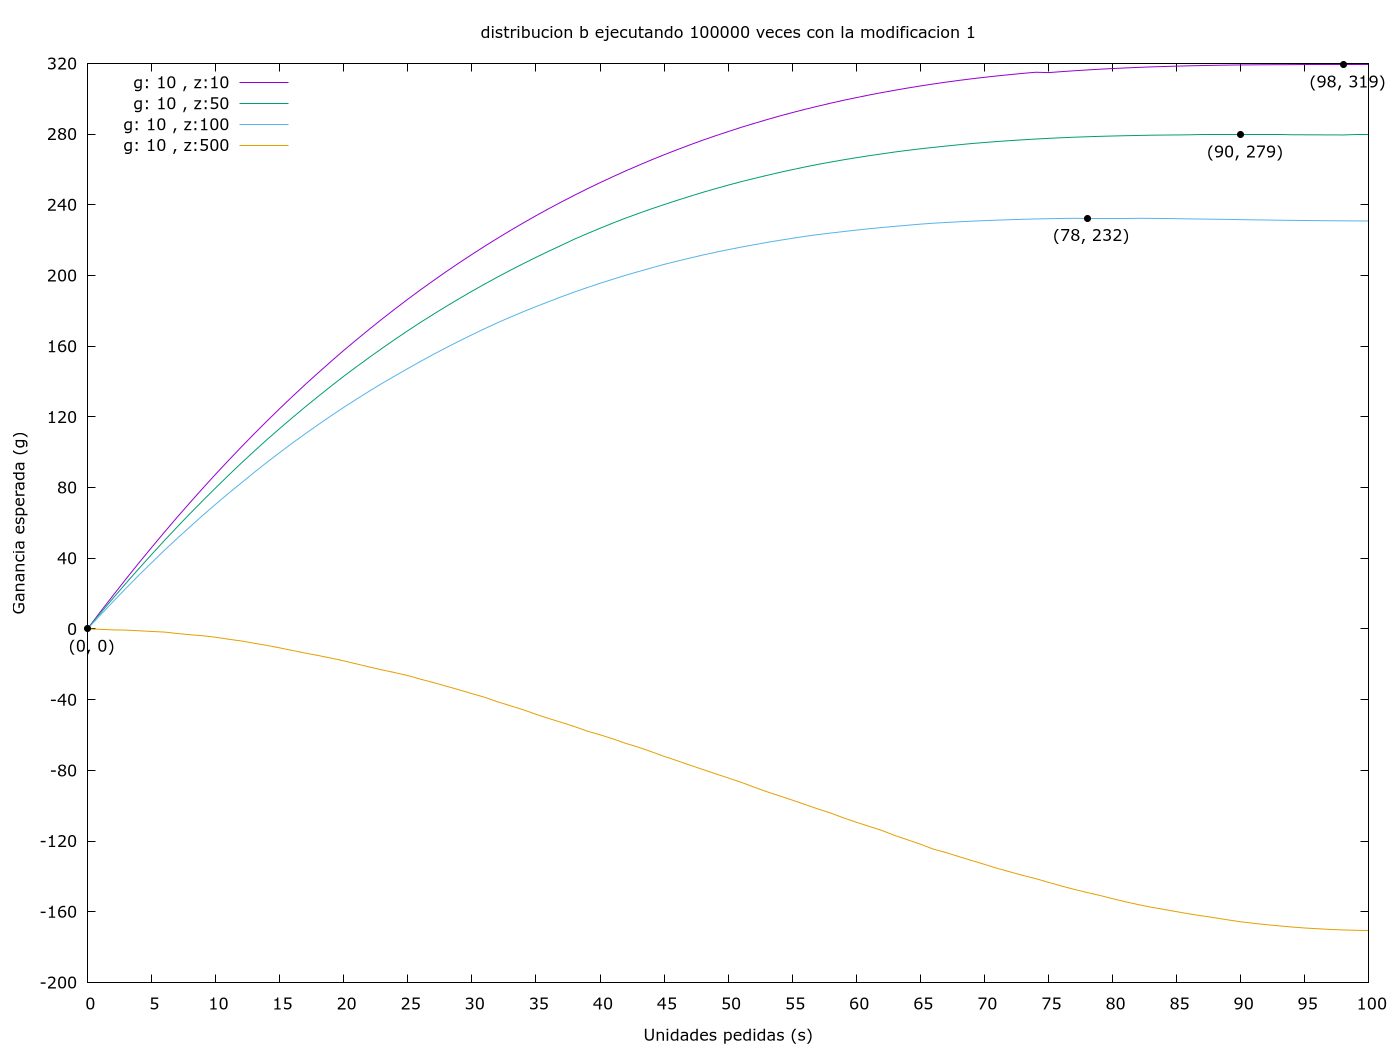
\includegraphics[scale = 0.2]{prob_b/datos_b_100000_1.png}
	\caption{Con 100000 repeticiones, la distribución b y la modificación 1.}
	\label{fig:ej1_a_100000}

\end{figure}

\begin{figure}[H]
	\centering
	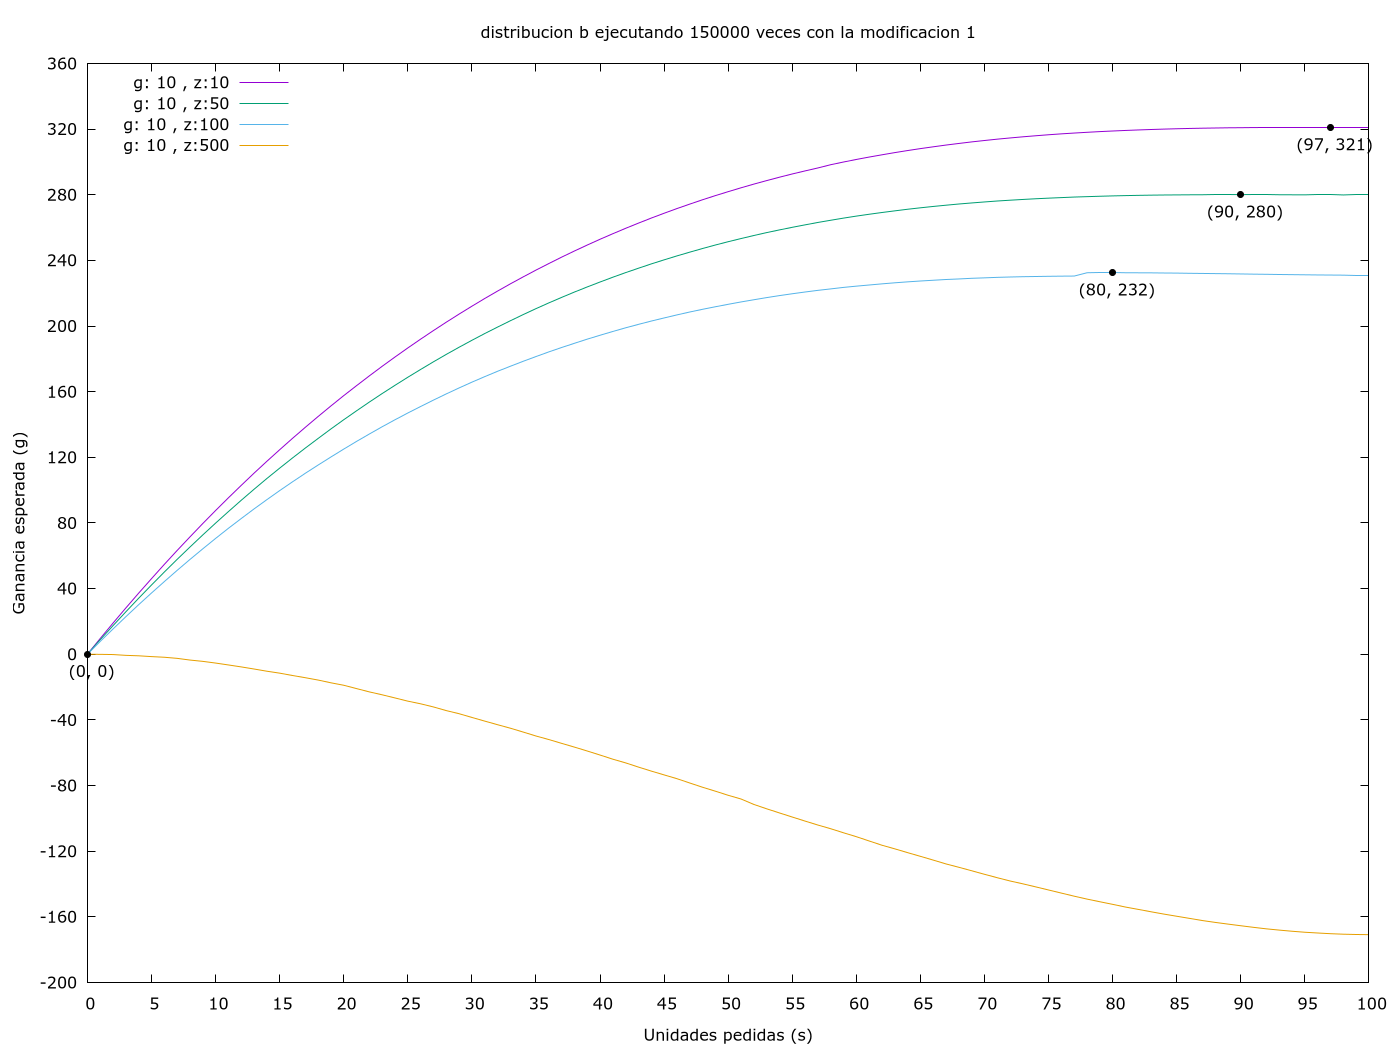
\includegraphics[scale = 0.2]{prob_b/datos_b_150000_1.png}
	\caption{Con 150000 repeticiones, la distribución b y la modificación 1.}
	\label{fig:ej1_a_150000}

\end{figure}


En este caso la naturaleza de como funciona esta modificación se ve mucho más clara. Al tener mayor probabilidad una demanda baja, cuando nos acercamos a muchas unidades pedidas, se estanca el valor de la ganancia ya que aunque no se vendan las unidades, el precio a pagar es siempre el mismo, por lo que a partir de las 70 unidades vendidas, vemos como es extraño vender más unidades, pero el vender alguna unidad extra nos supone una mayor ventaja que comprar 20 unidades pero quedarnos sin material a vender, ya que supone mayor riesgo el comprar menos y que se quede una única sin vender, rebajaría la ganancia.

También observamos que en el caso $z = 500$ el precio de devolución es tan alto que es mejor no contratar ninguna unidad, ya que por alta que sea la probabilidad de venderla, si una unidad no es vendida las perdidas serían mucho mayores.

\subsubsection{Resultados obtenidos con la distribución c}



\begin{figure}[H]
	\centering
	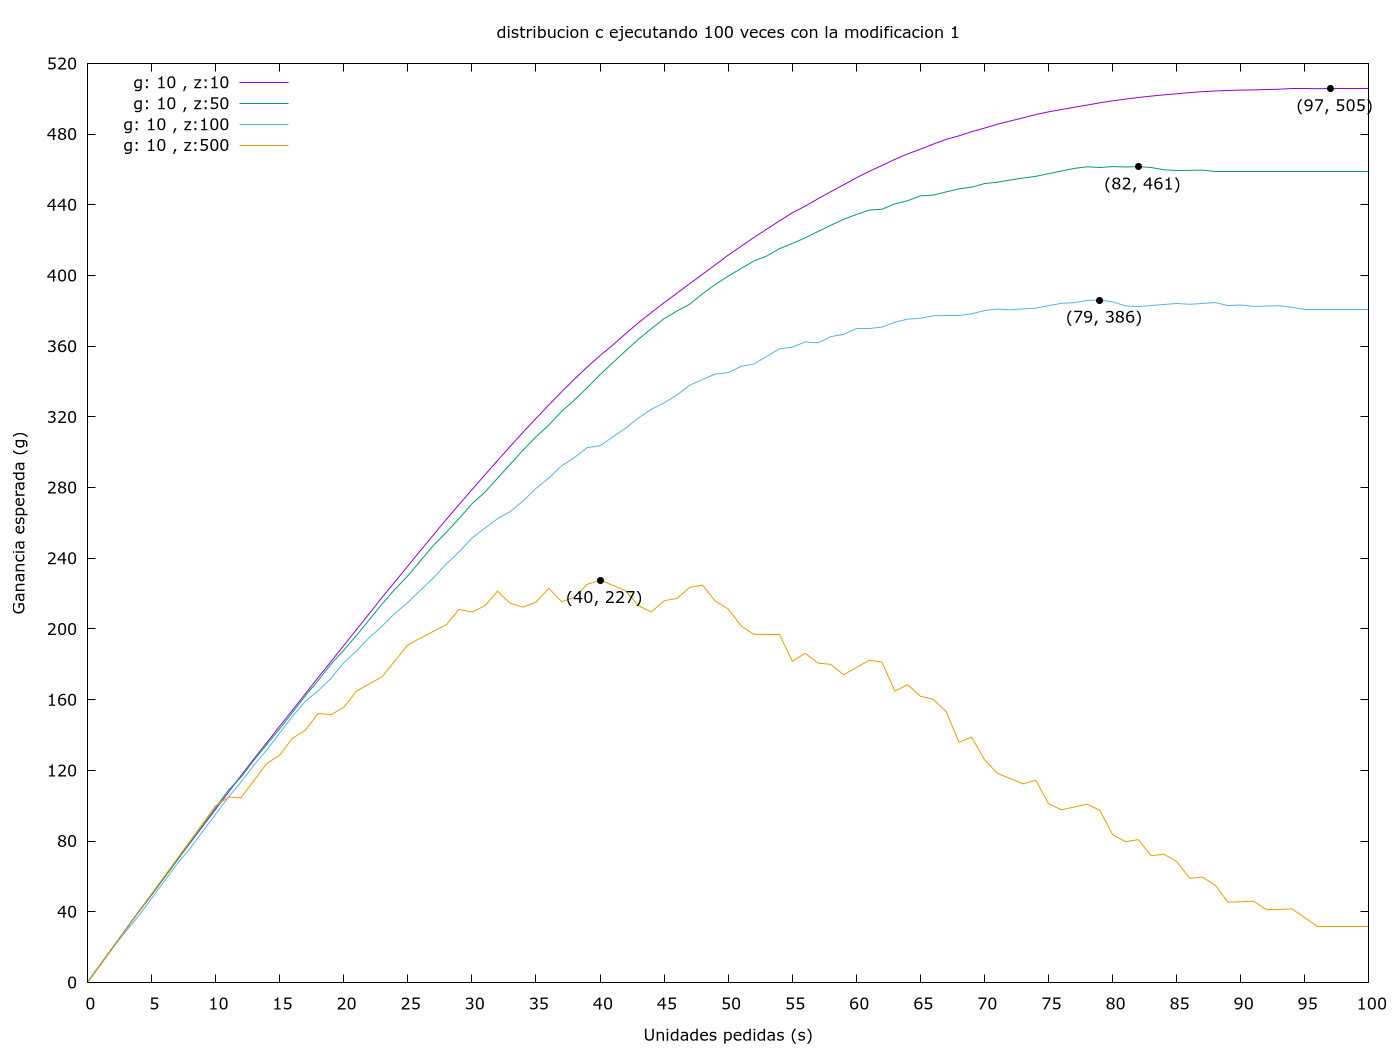
\includegraphics[scale = 0.2]{prob_c/datos_c_100_1.png}
	\caption{Con 100 repeticiones, la distribución b y la modificación 1.}
	\label{fig:ej1_a_100}

\end{figure}

\begin{figure}[H]
	\centering
	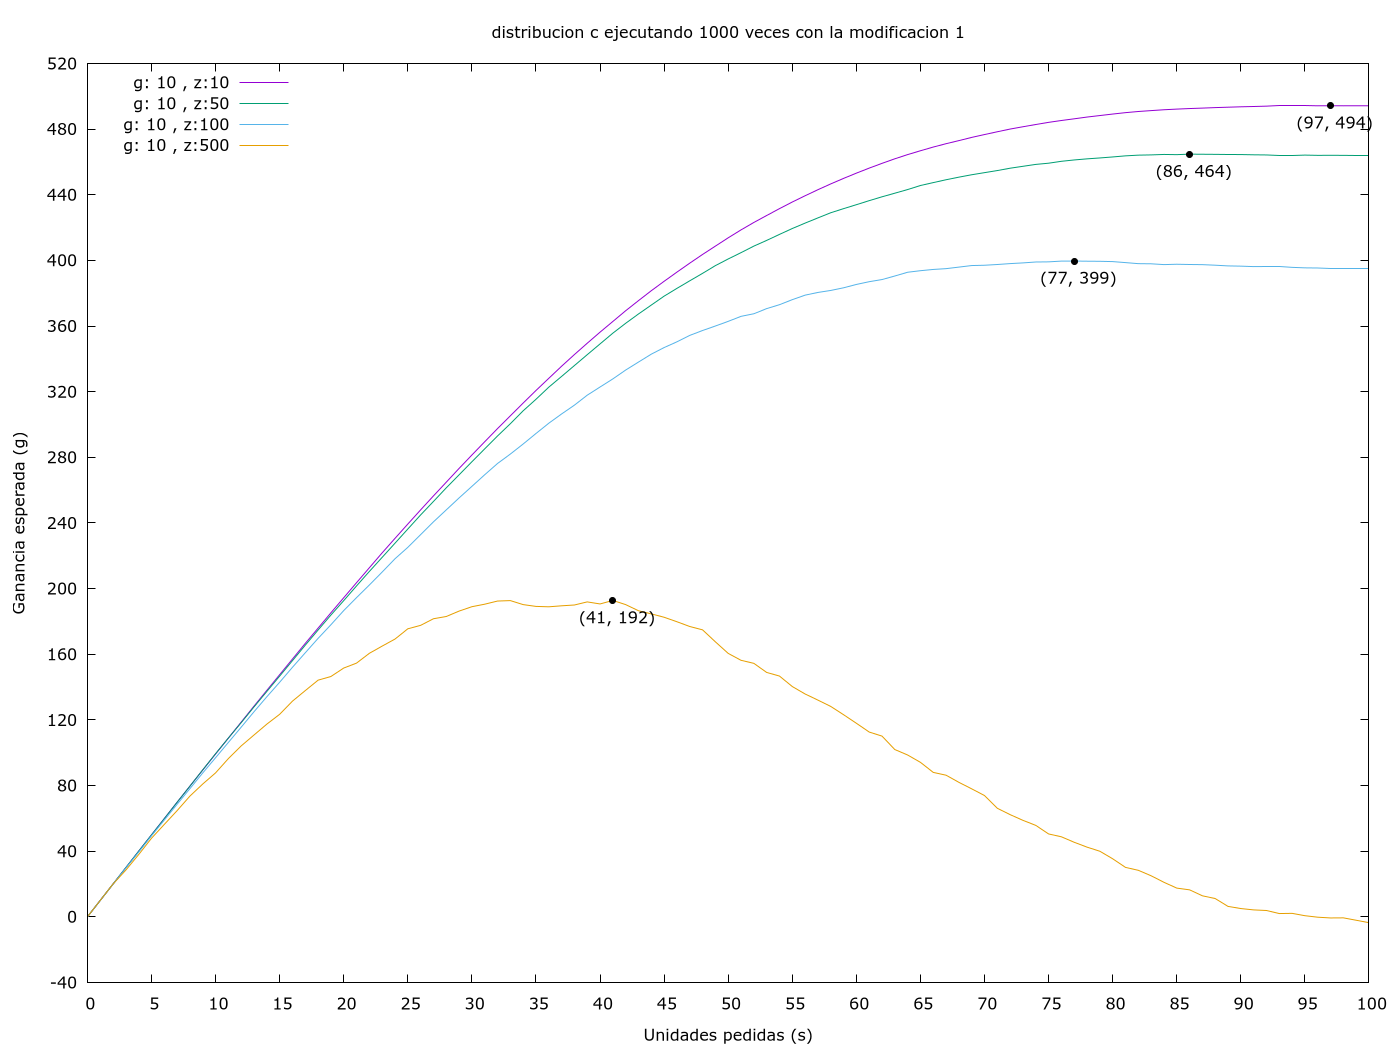
\includegraphics[scale = 0.2]{prob_c/datos_c_1000_1.png}
	\caption{Con 1000 repeticiones, la distribución b y la modificación 1.}
	\label{fig:ej1_a_1000}

\end{figure}

\begin{figure}[H]
	\centering
	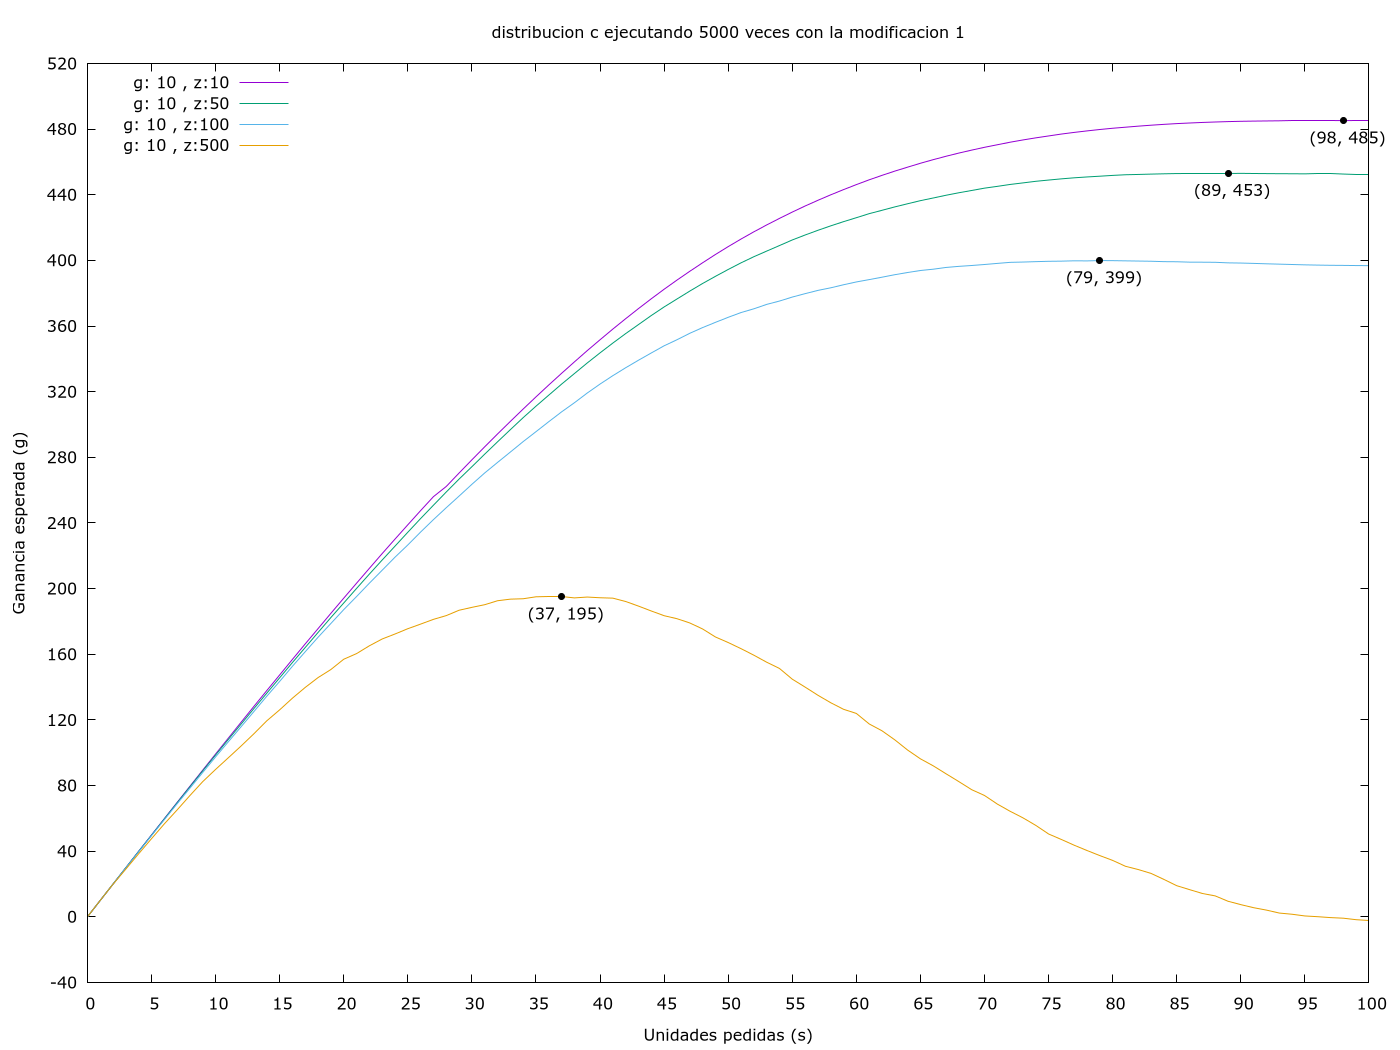
\includegraphics[scale = 0.2]{prob_c/datos_c_5000_1.png}
	\caption{Con 5000 repeticiones, la distribución b y la modificación 1.}
	\label{fig:ej1_a_5000}

\end{figure}


\begin{figure}[H]
	\centering
	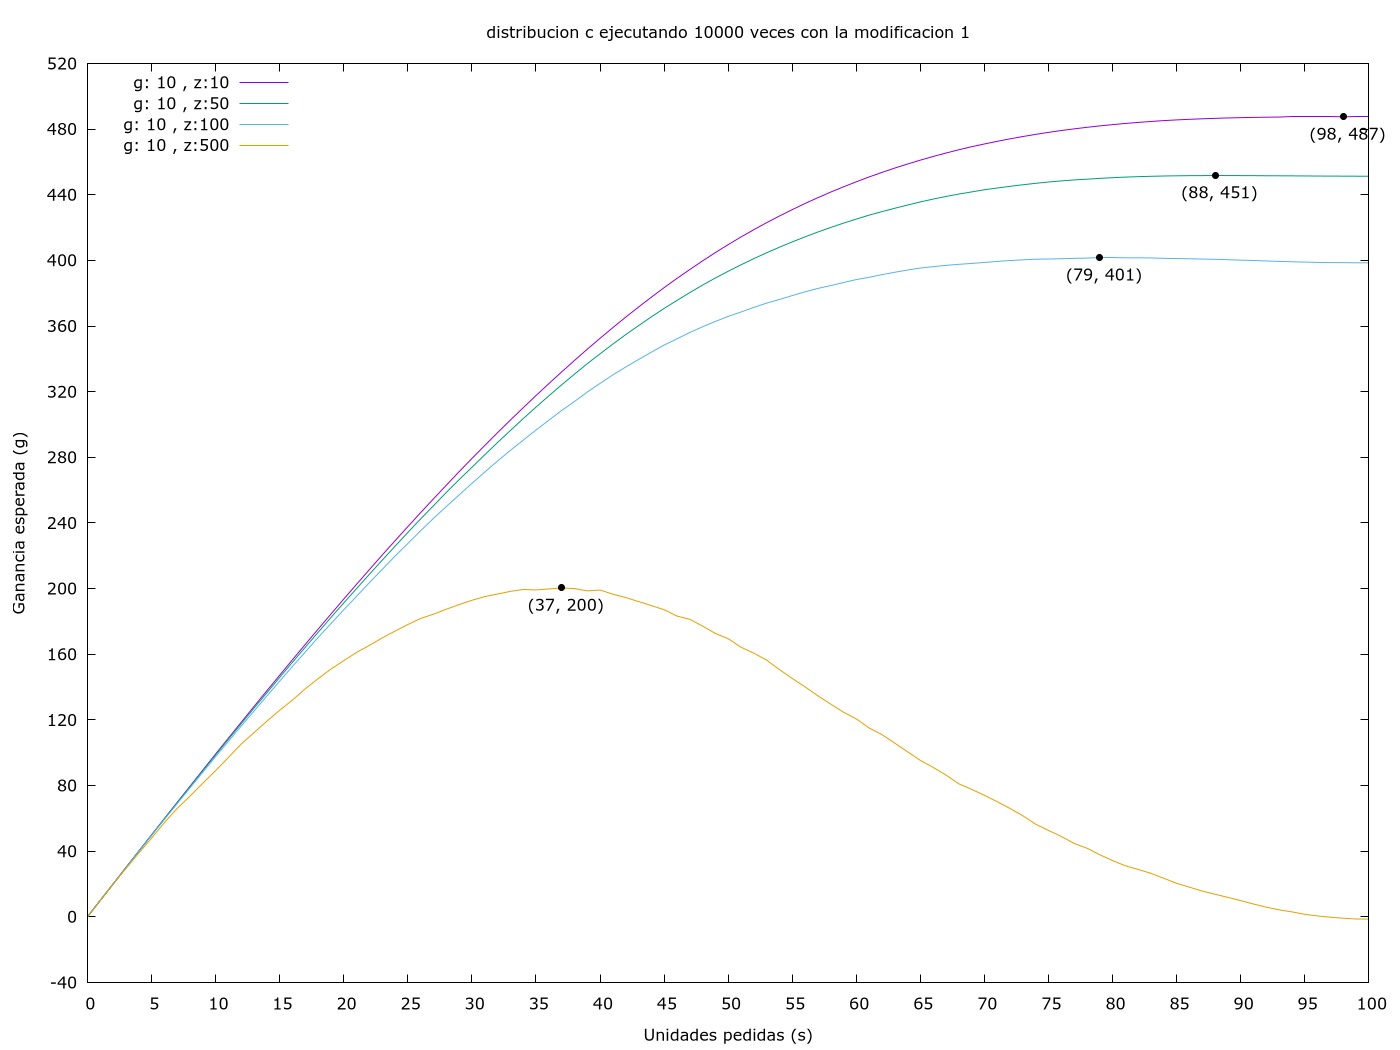
\includegraphics[scale = 0.2]{prob_c/datos_c_10000_1.png}
	\caption{Con 10000 repeticiones, la distribución b y la modificación 1.}
	\label{fig:ej1_a_10000}

\end{figure}

\begin{figure}[H]
	\centering
	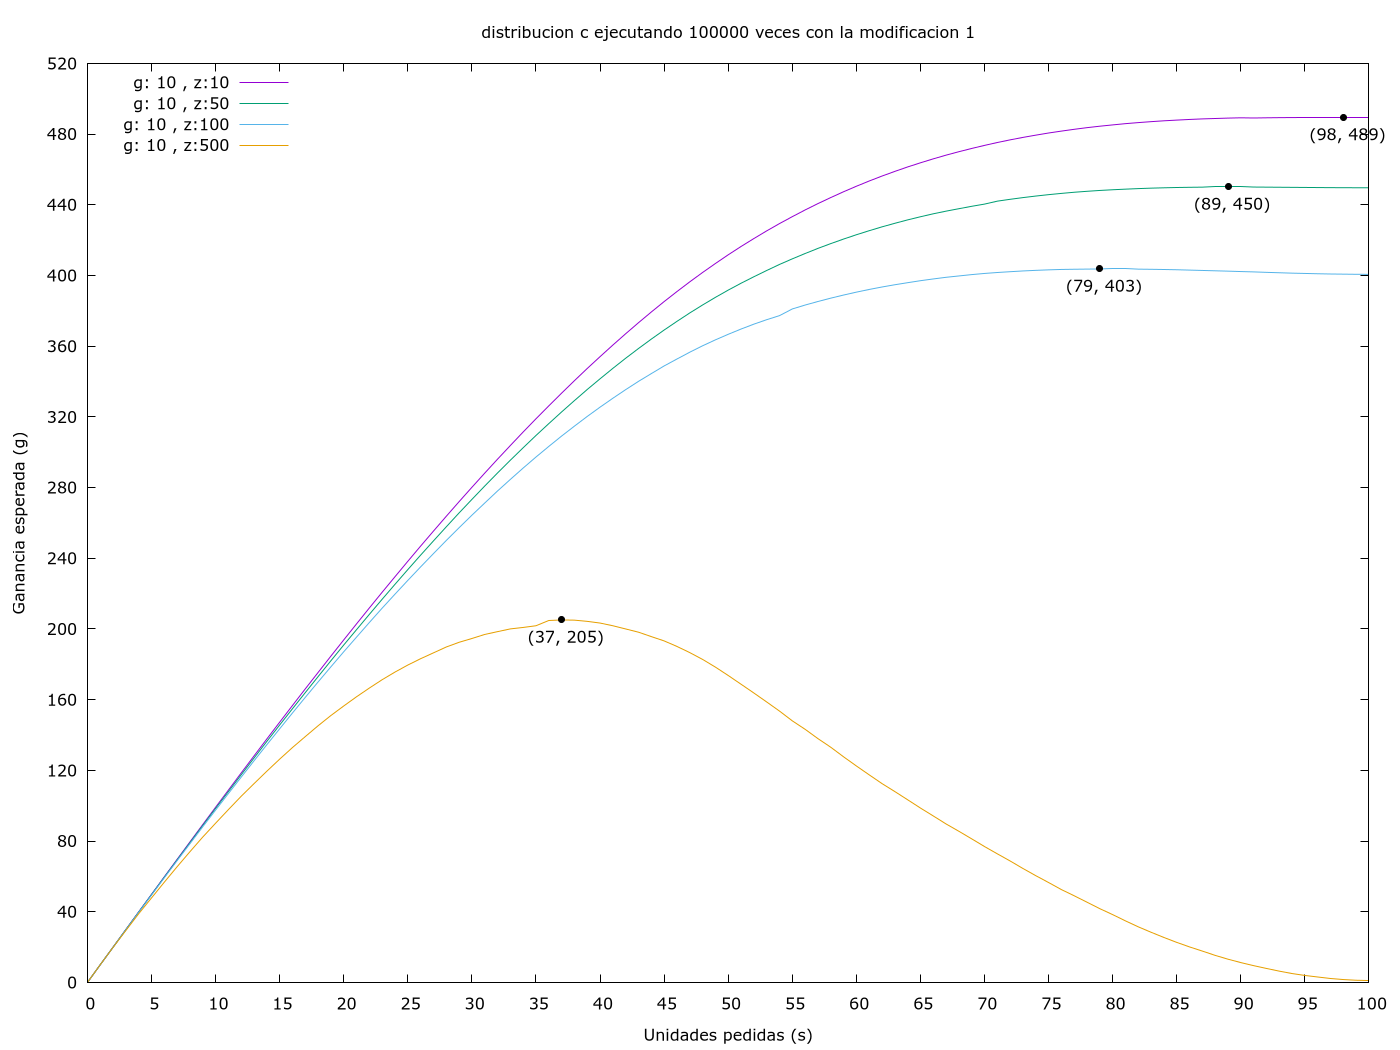
\includegraphics[scale = 0.2]{prob_c/datos_c_100000_1.png}
	\caption{Con 100000 repeticiones, la distribución b y la modificación 1.}
	\label{fig:ej1_a_100000}

\end{figure}

\begin{figure}[H]
	\centering
	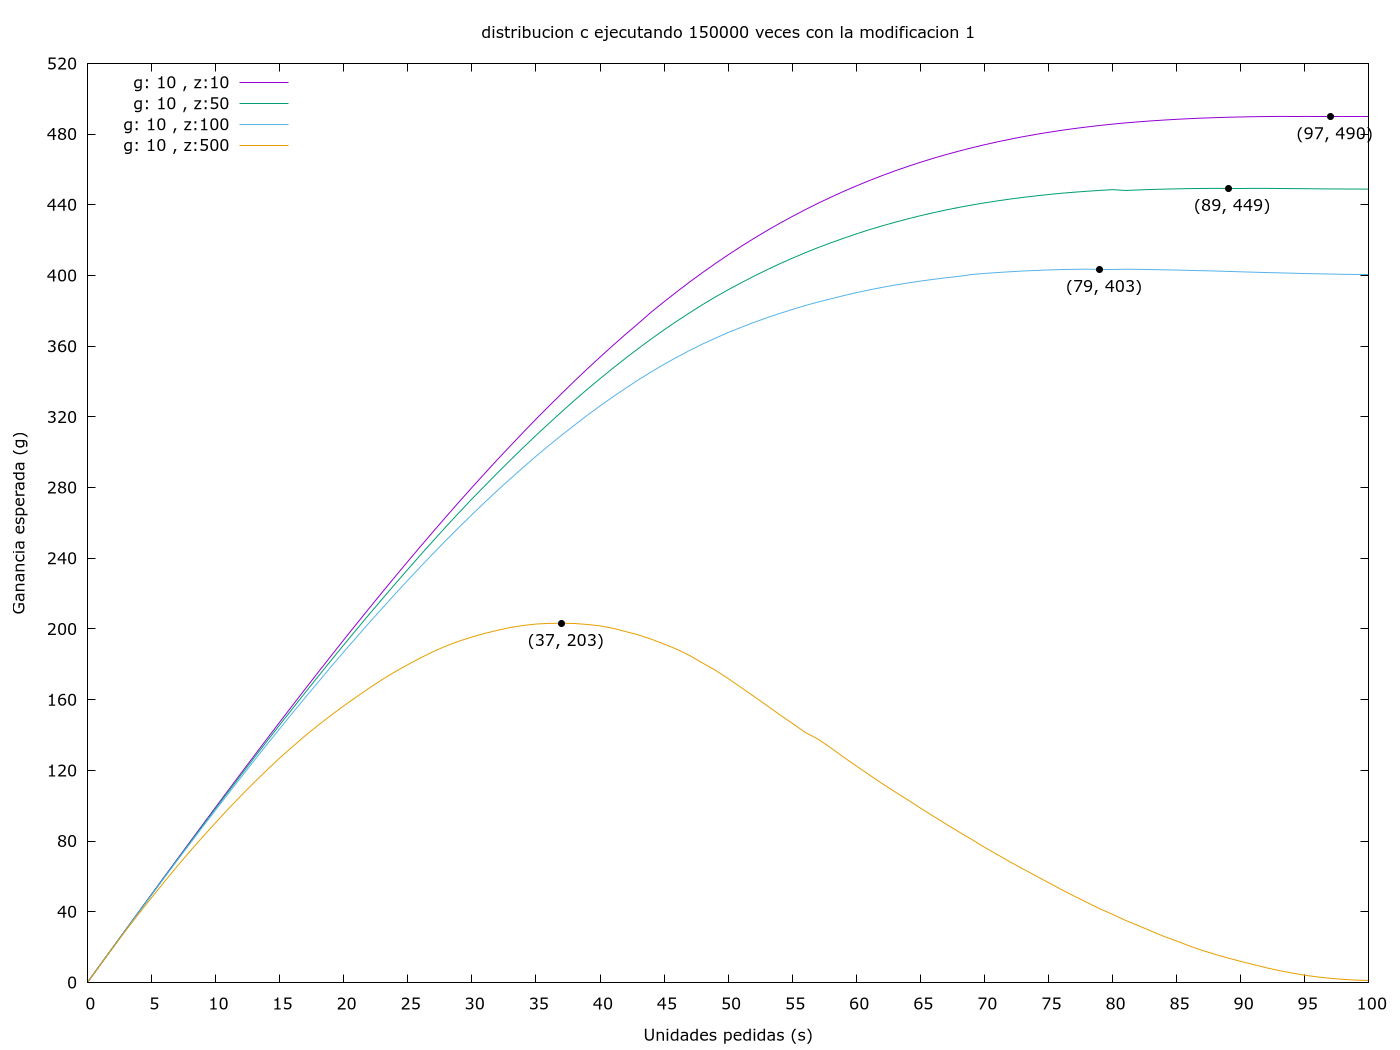
\includegraphics[scale = 0.2]{prob_c/datos_c_150000_1.png}
	\caption{Con 150000 repeticiones, la distribución b y la modificación 1.}
	\label{fig:ej1_a_150000}

\end{figure}

En esta situación observamos que solventamos el problema que teniamos sin la modificación, ya que la distribución triangular nos permite tener altas ganancias hasta llegar a la mitad de unidades máximas, y a partir de ese punto mantenernos como en el caso de la distribución b, sin embargo esta distribución nos permite contratar más unidades para obtener una mayor ganancia ya que los valores mayores que 70 siguen teniendo una probabilidad alta en comparación con la distribución b.

El único problema sería en el caso de que el coste de devolución sea muy alto, en el que rebajaría mucho la ganancia obtenida, sin embargo es el caso más opimista de todos los estudiados, ya que incluso siendo bastante pesimista y alto el coste de no vender un único periódico no llegaría a producir pérdidas en ningún caso.



\subsection{Modificación 2 del modelo}

De nuevo se nos pide una última modificación, en este caso se permite escoger si asumir el gasto por unidad vendida o si realizar un único pago como devolución, por lo tanto el coste de devolución será el mínimo entre las unidades no vendidas por el coste de no vender una unidad y el pago del precio fijo $z$.

Experimentaremos con los mismos valores de $z$ y de $y$ que en el apartado sin modificaciones y en el anterior.

\subsubsection{Resultados obtenidos con la distribución a}


\begin{figure}[H]
	\centering
	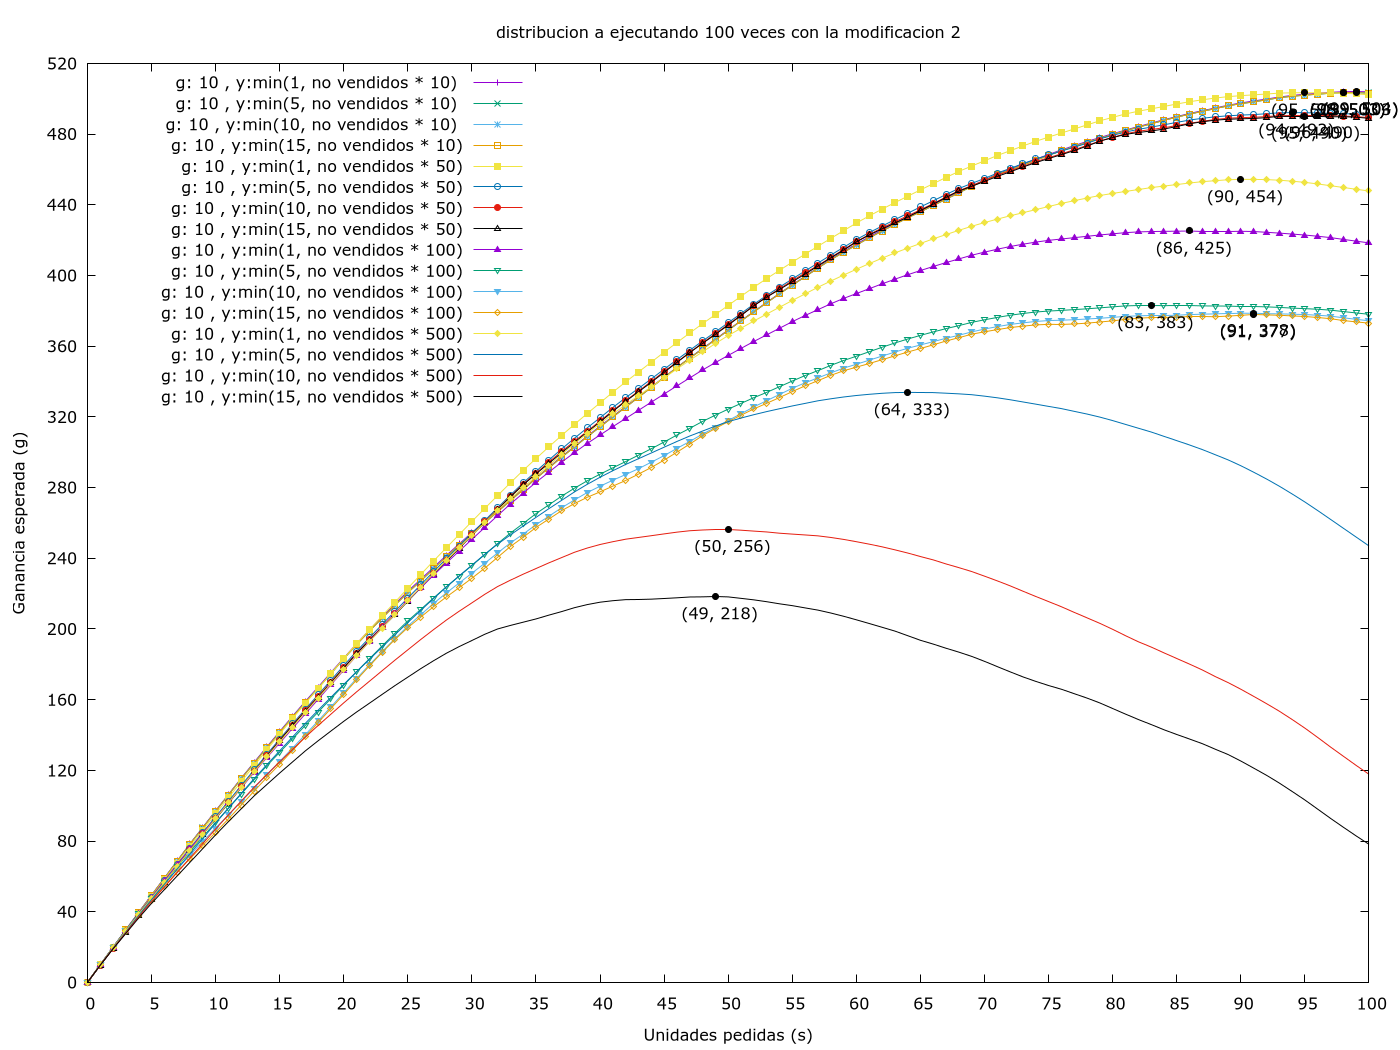
\includegraphics[scale = 0.2]{prob_a/datos_a_100_2.png}
	\caption{Con 100 repeticiones, la distribución a y la modificación 2.}
	\label{fig:ej1_a_100}

\end{figure}

\begin{figure}[H]
	\centering
	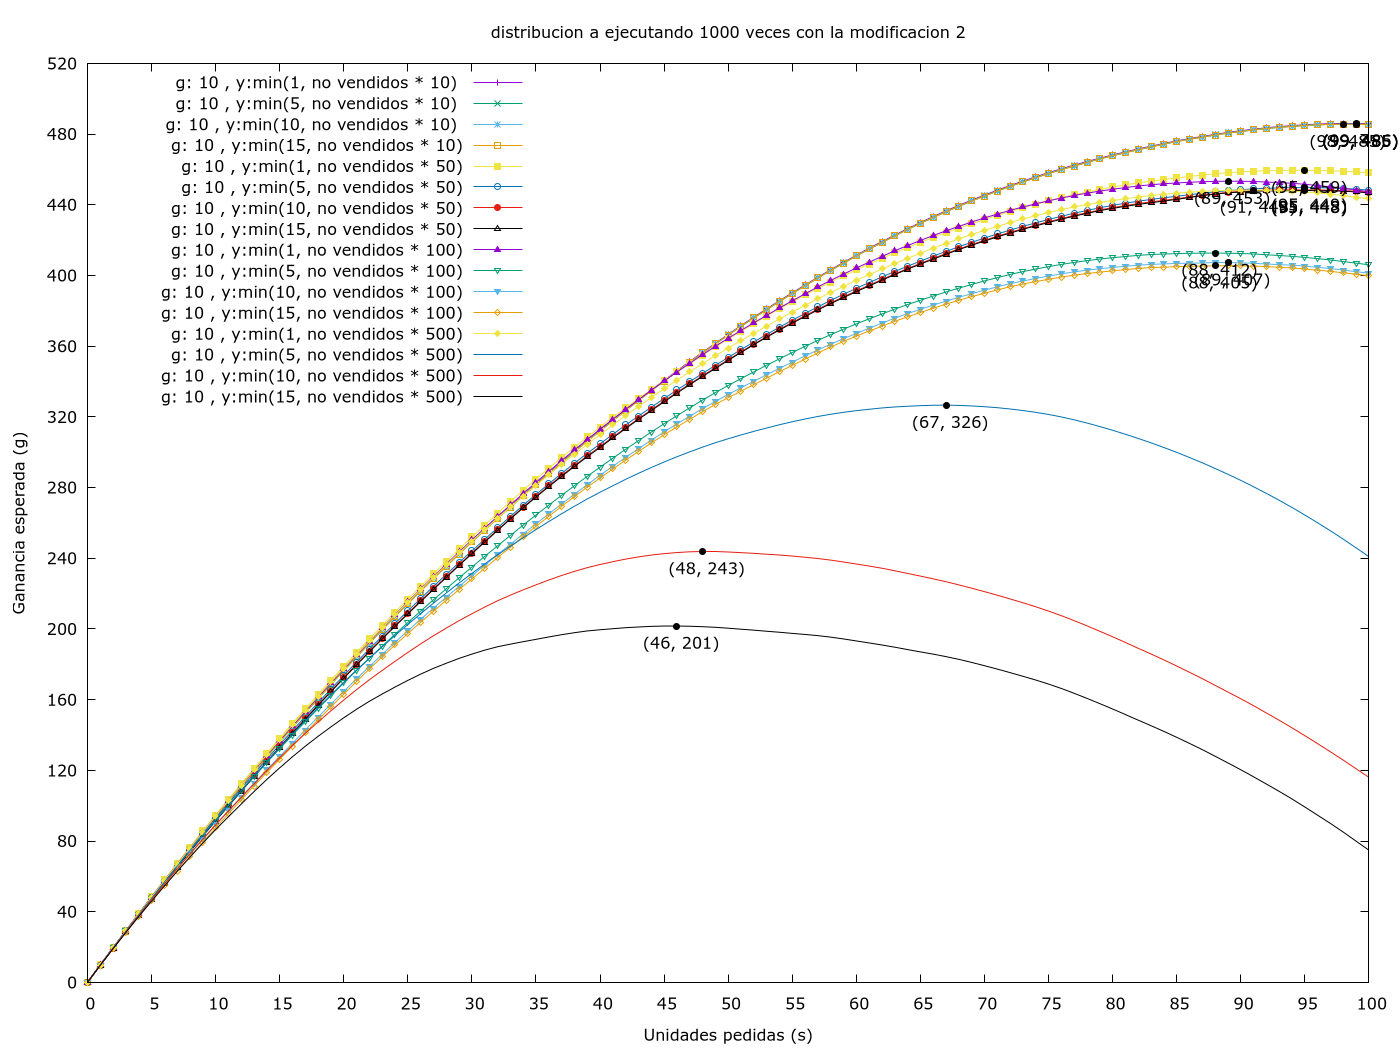
\includegraphics[scale = 0.2]{prob_a/datos_a_1000_2.png}
	\caption{Con 1000 repeticiones, la distribución a y la modificación 2.}
	\label{fig:ej1_a_1000}

\end{figure}

\begin{figure}[H]
	\centering
	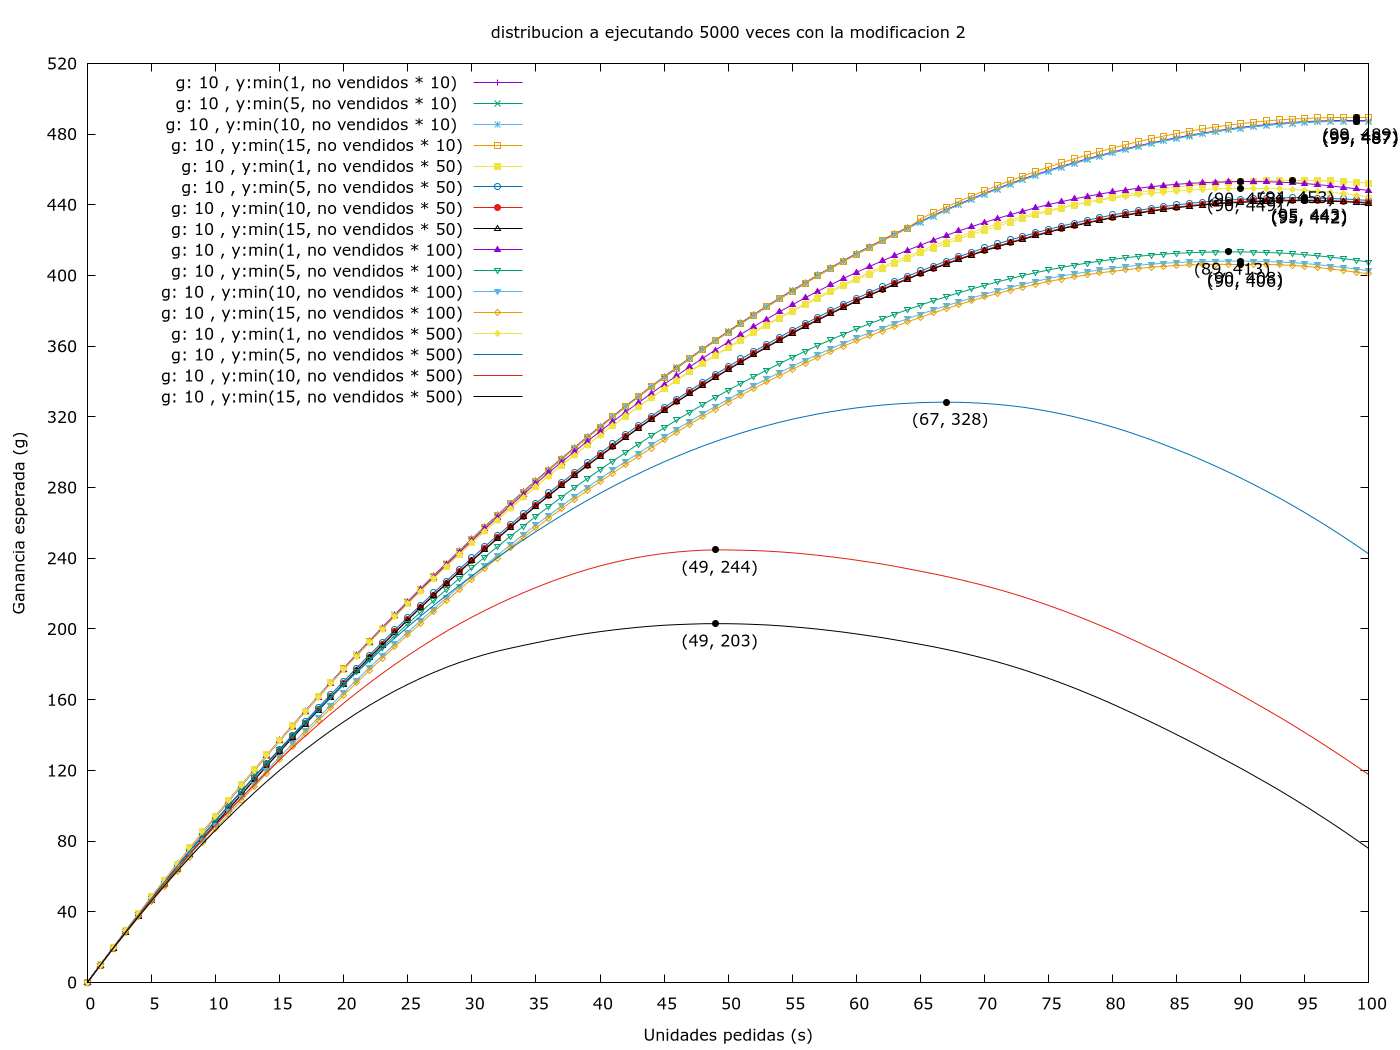
\includegraphics[scale = 0.2]{prob_a/datos_a_5000_2.png}
	\caption{Con 5000 repeticiones, la distribución a y la modificación 2.}
	\label{fig:ej1_a_5000}

\end{figure}


\begin{figure}[H]
	\centering
	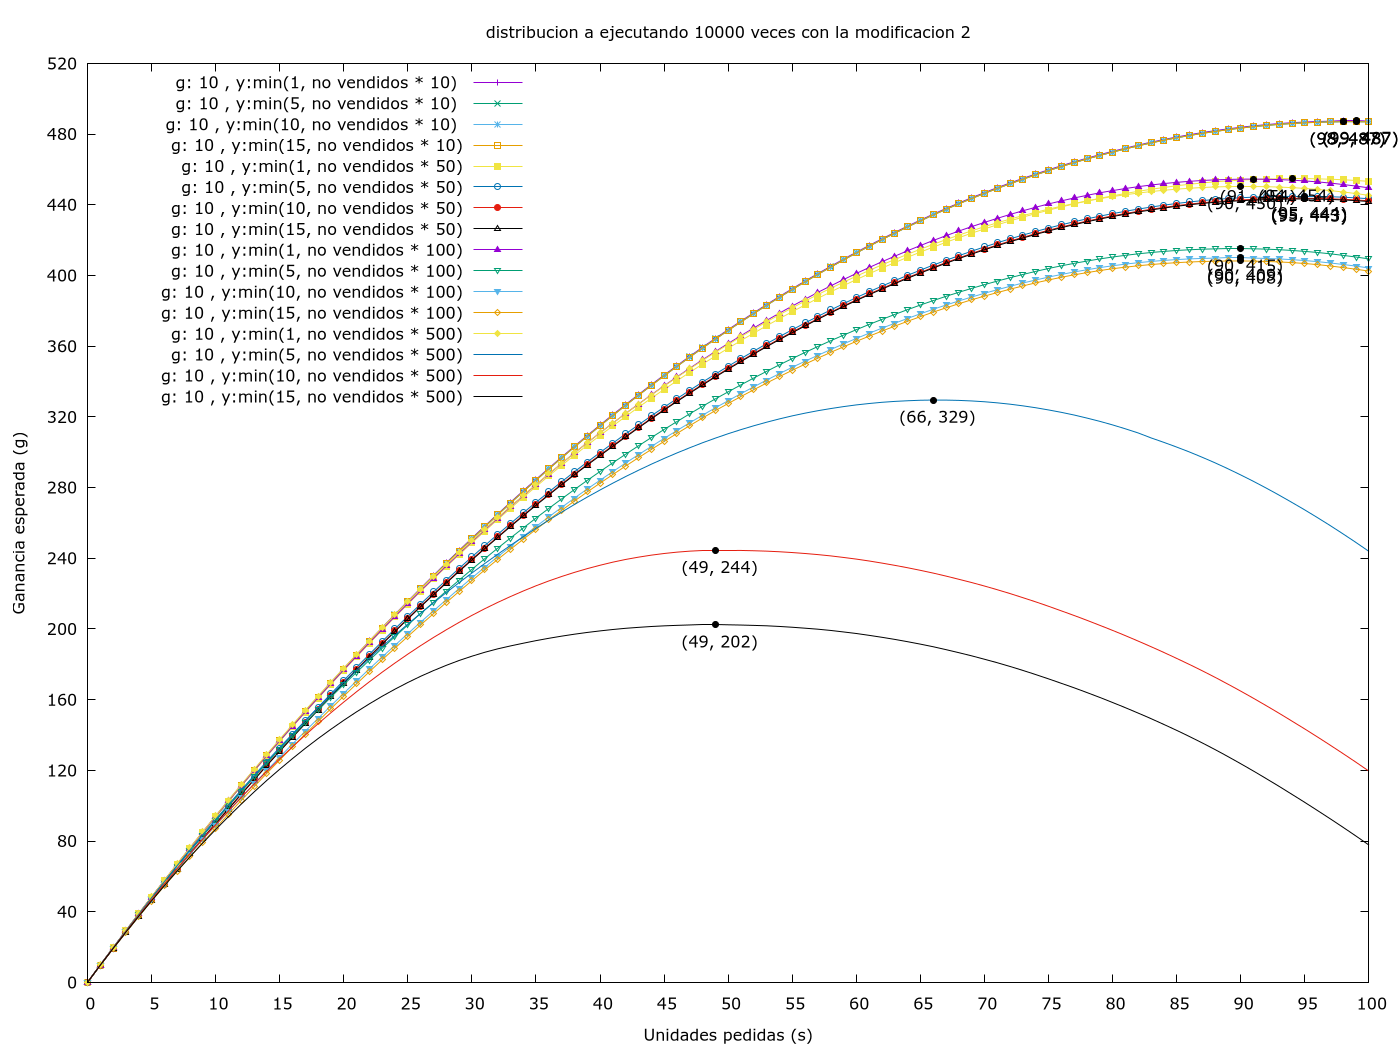
\includegraphics[scale = 0.2]{prob_a/datos_a_10000_2.png}
	\caption{Con 10000 repeticiones, la distribución a y la modificación 2.}
	\label{fig:ej1_a_10000}

\end{figure}

\begin{figure}[H]
	\centering
	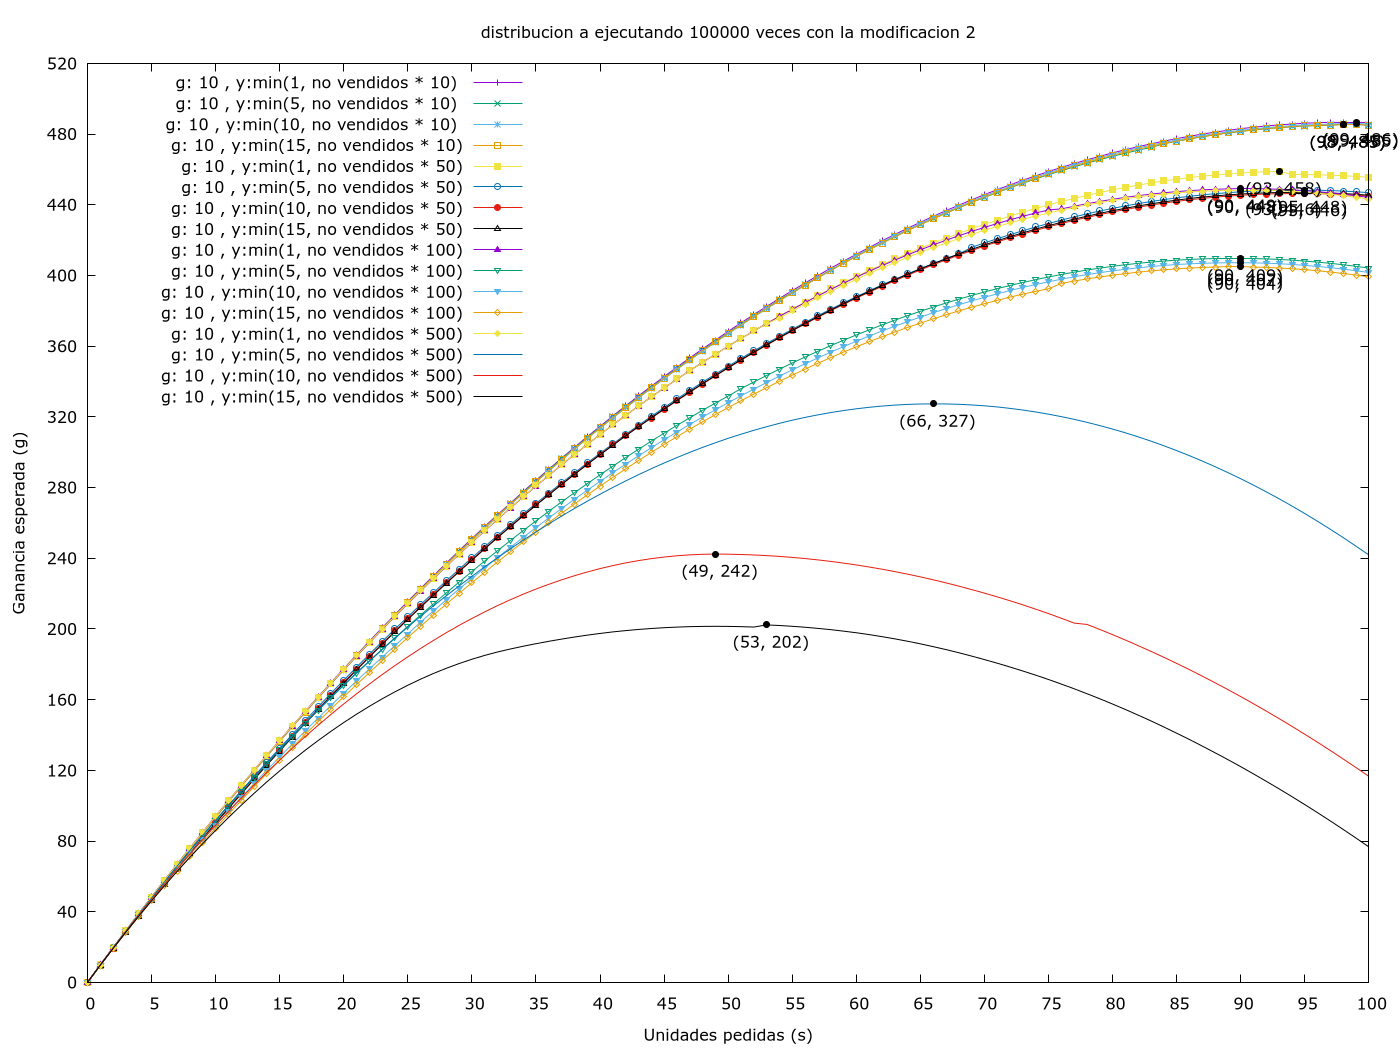
\includegraphics[scale = 0.2]{prob_a/datos_a_100000_2.png}
	\caption{Con 100000 repeticiones, la distribución a y la modificación 2.}
	\label{fig:ej1_a_100000}

\end{figure}

\begin{figure}[H]
	\centering
	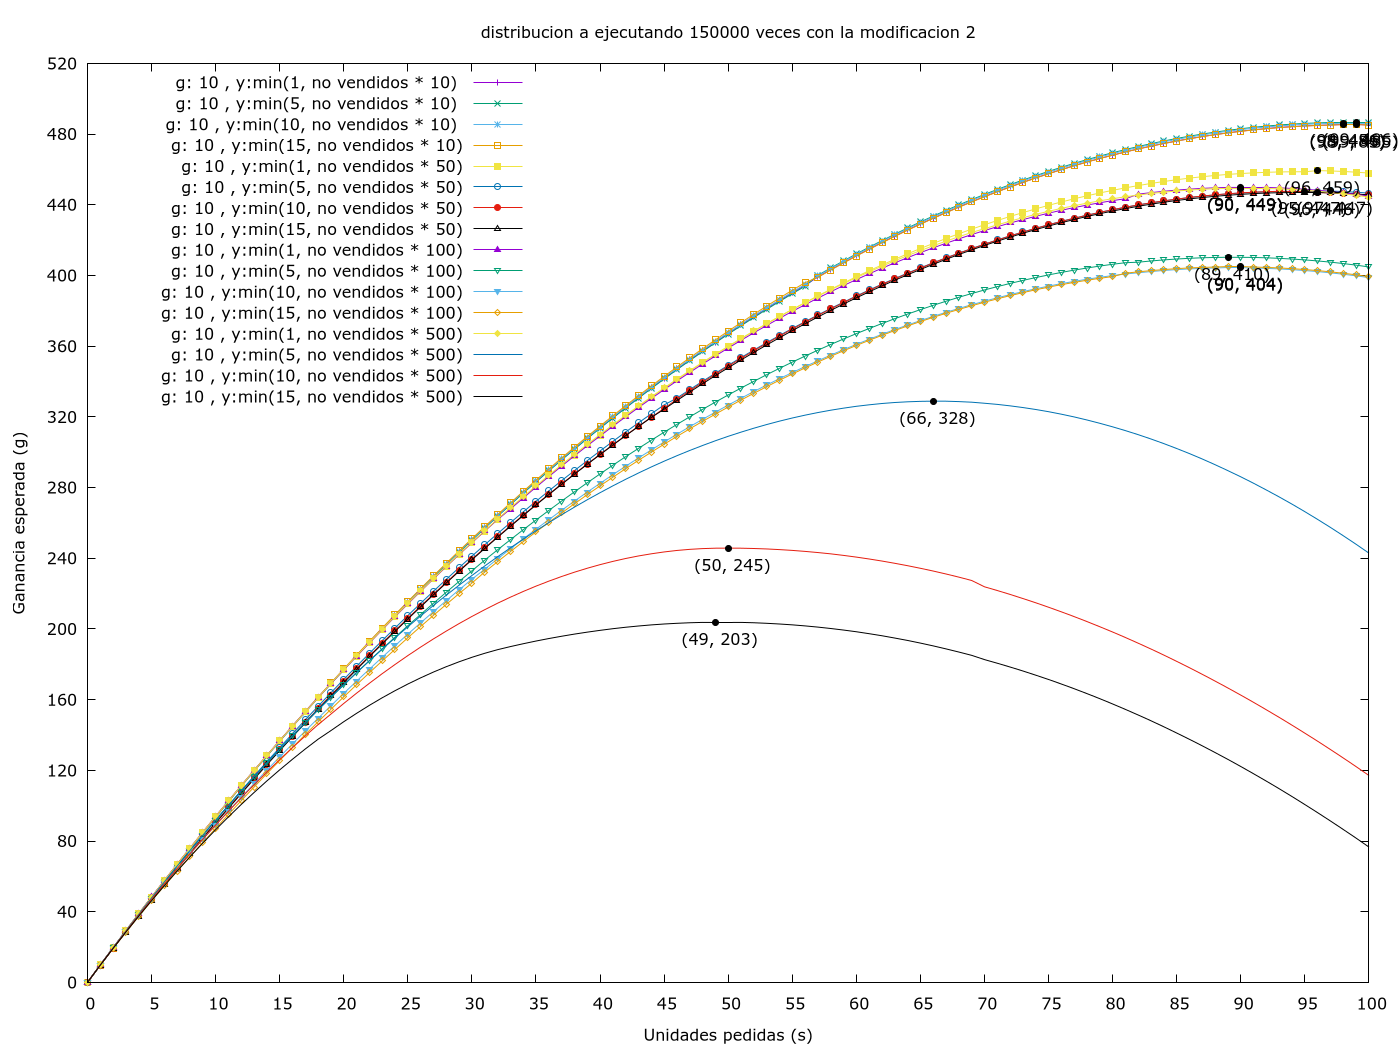
\includegraphics[scale = 0.2]{prob_a/datos_a_150000_2.png}
	\caption{Con 150000 repeticiones, la distribución a y la modificación 2.}
	\label{fig:ej1_a_150000}

\end{figure}

Con esta nueva modificación vemos que para esta distribución nunca se realizan pérdidas, ya que el poder elegir entre si pagar por cada unidad no vendida o si un único pago, haciendo que en los casos que queden muchas unidades sin vender, no se llegue a pagar tanto como para entrar en pérdidas.

También observamos qeue mantenemos unos óptimos de unidades que nos aportan bastantes ganancias, incluso en los casos que nos suponen un mayor coste de devolución.

\subsubsection{Resultados obtenidos con la distribución b}


\begin{figure}[H]
	\centering
	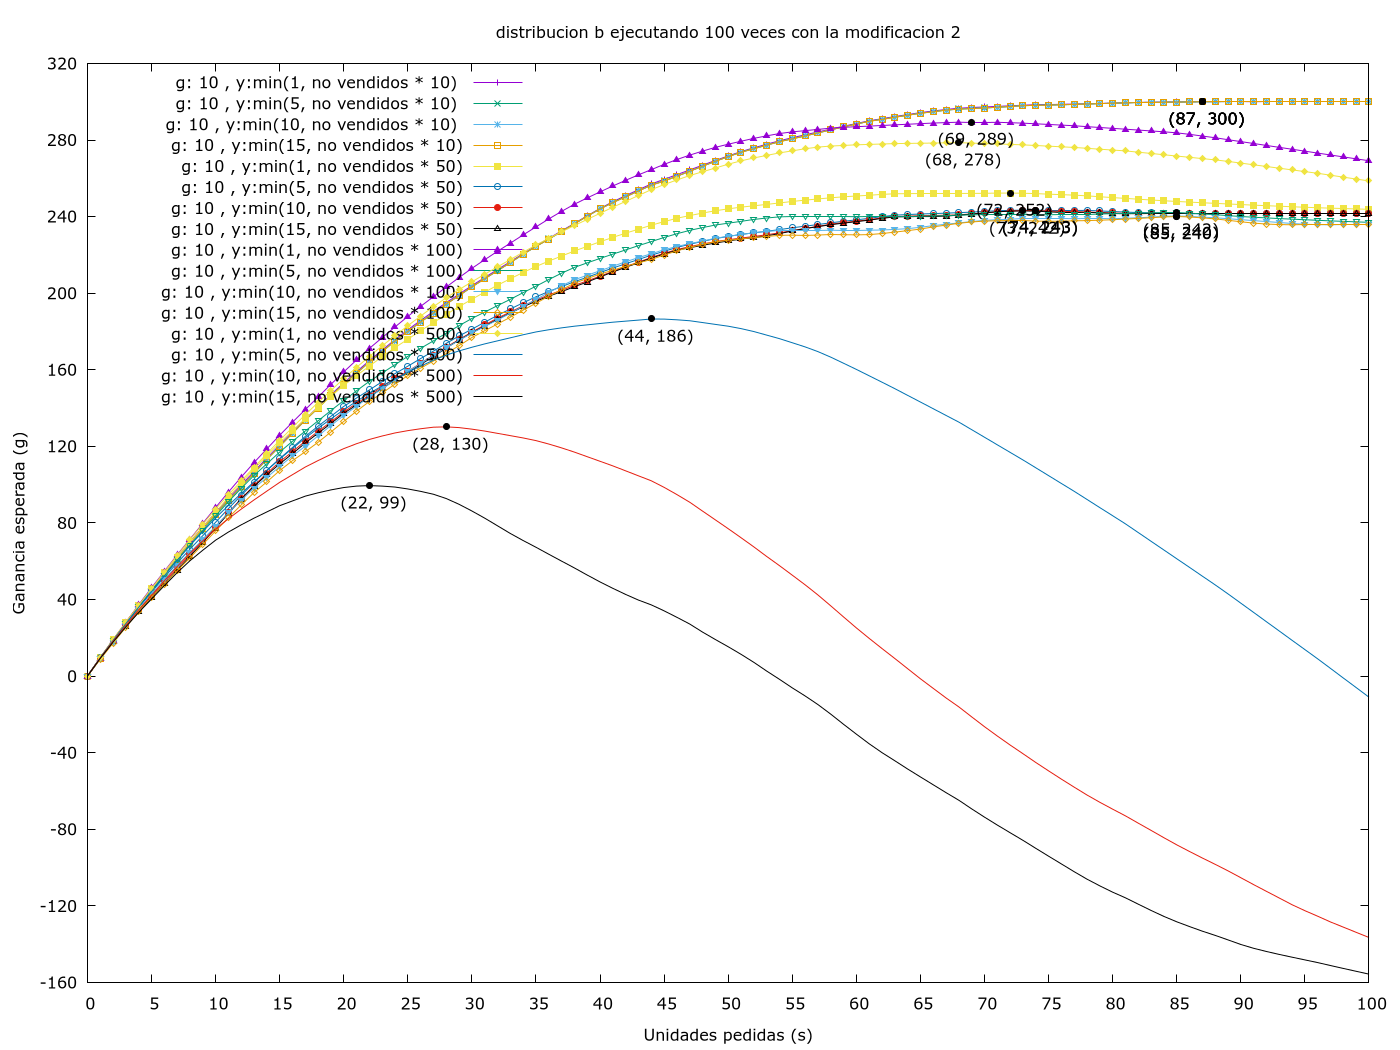
\includegraphics[scale = 0.2]{prob_b/datos_b_100_2.png}
	\caption{Con 100 repeticiones, la distribución b y la modificación 2.}
	\label{fig:ej1_a_100}

\end{figure}

\begin{figure}[H]
	\centering
	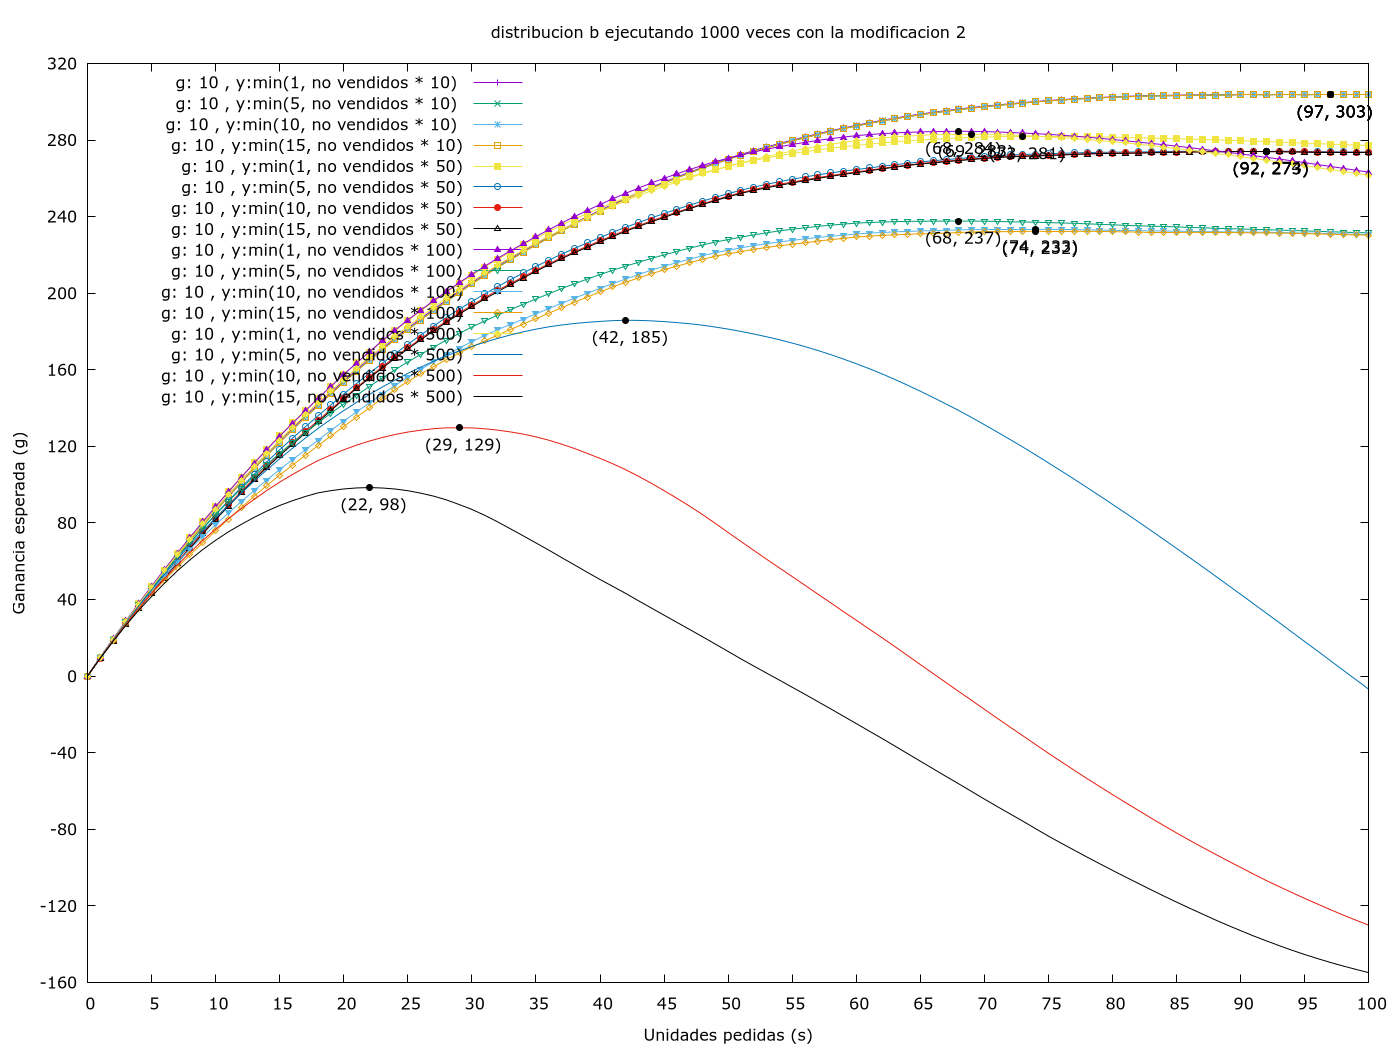
\includegraphics[scale = 0.2]{prob_b/datos_b_1000_2.png}
	\caption{Con 1000 repeticiones, la distribución b y la modificación 2.}
	\label{fig:ej1_a_1000}

\end{figure}

\begin{figure}[H]
	\centering
	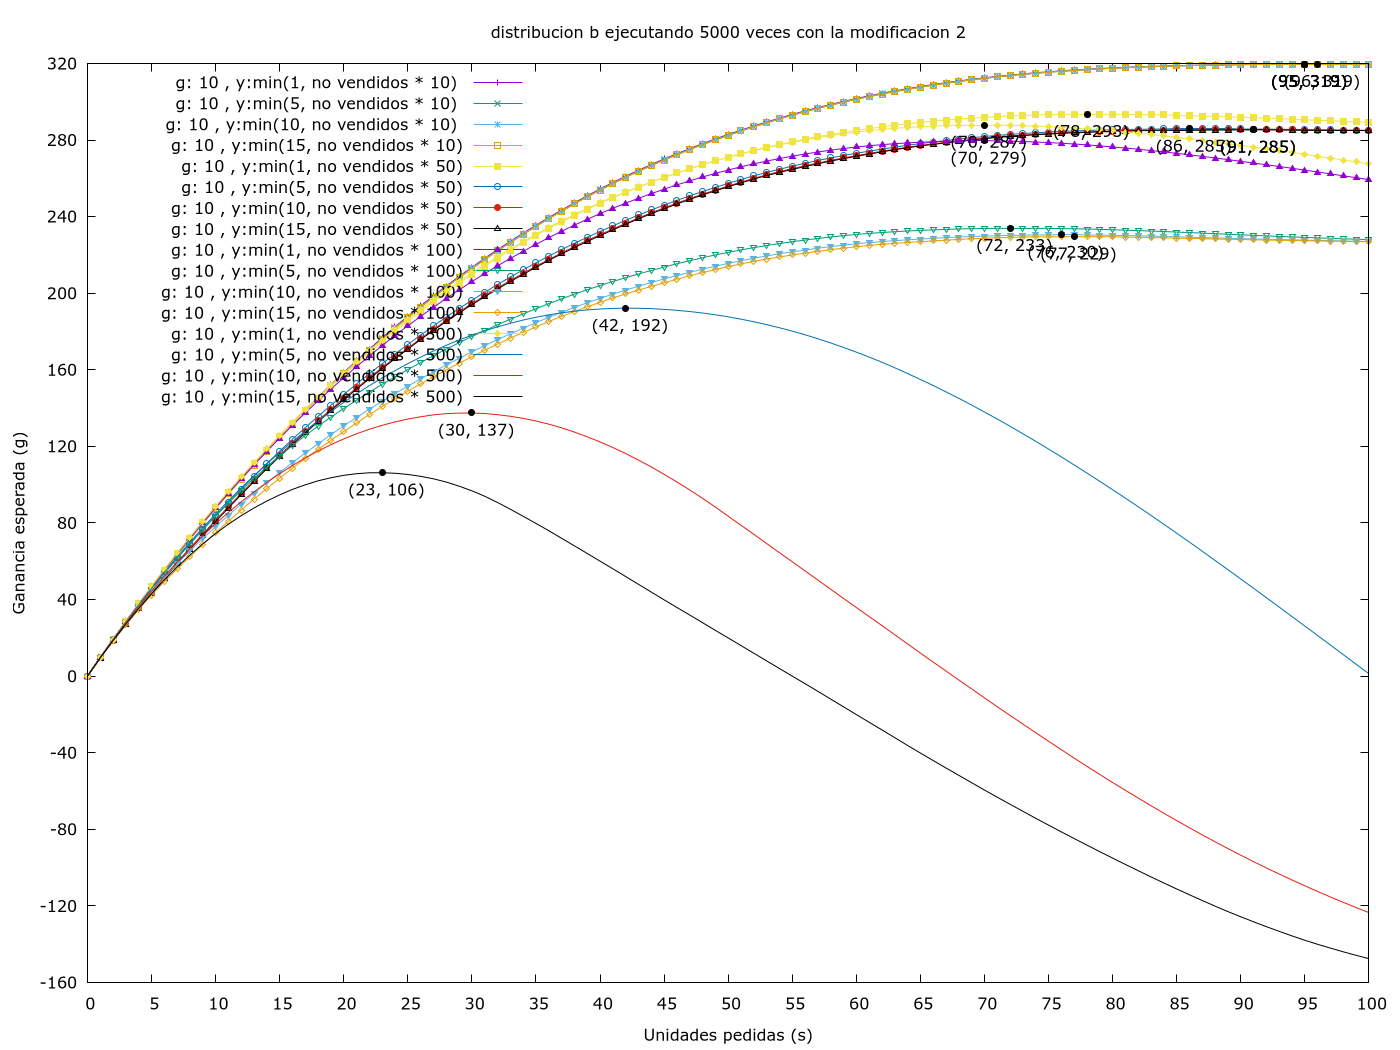
\includegraphics[scale = 0.2]{prob_b/datos_b_5000_2.png}
	\caption{Con 5000 repeticiones, la distribución b y la modificación 2.}
	\label{fig:ej1_a_5000}

\end{figure}


\begin{figure}[H]
	\centering
	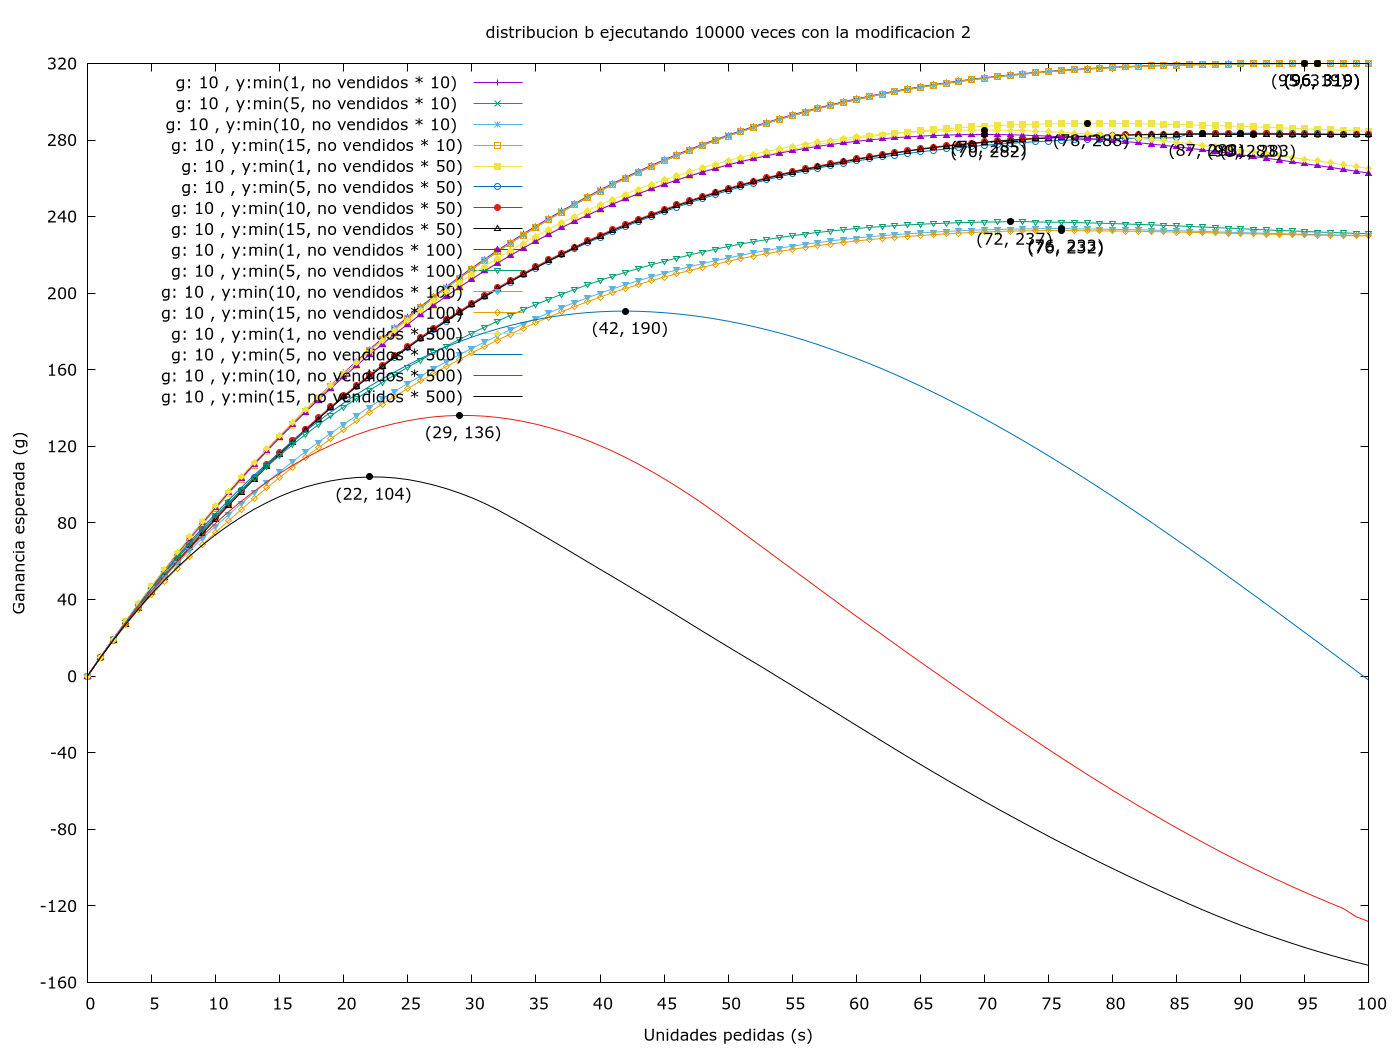
\includegraphics[scale = 0.2]{prob_b/datos_b_10000_2.png}
	\caption{Con 10000 repeticiones, la distribución b y la modificación 2.}
	\label{fig:ej1_a_10000}

\end{figure}

\begin{figure}[H]
	\centering
	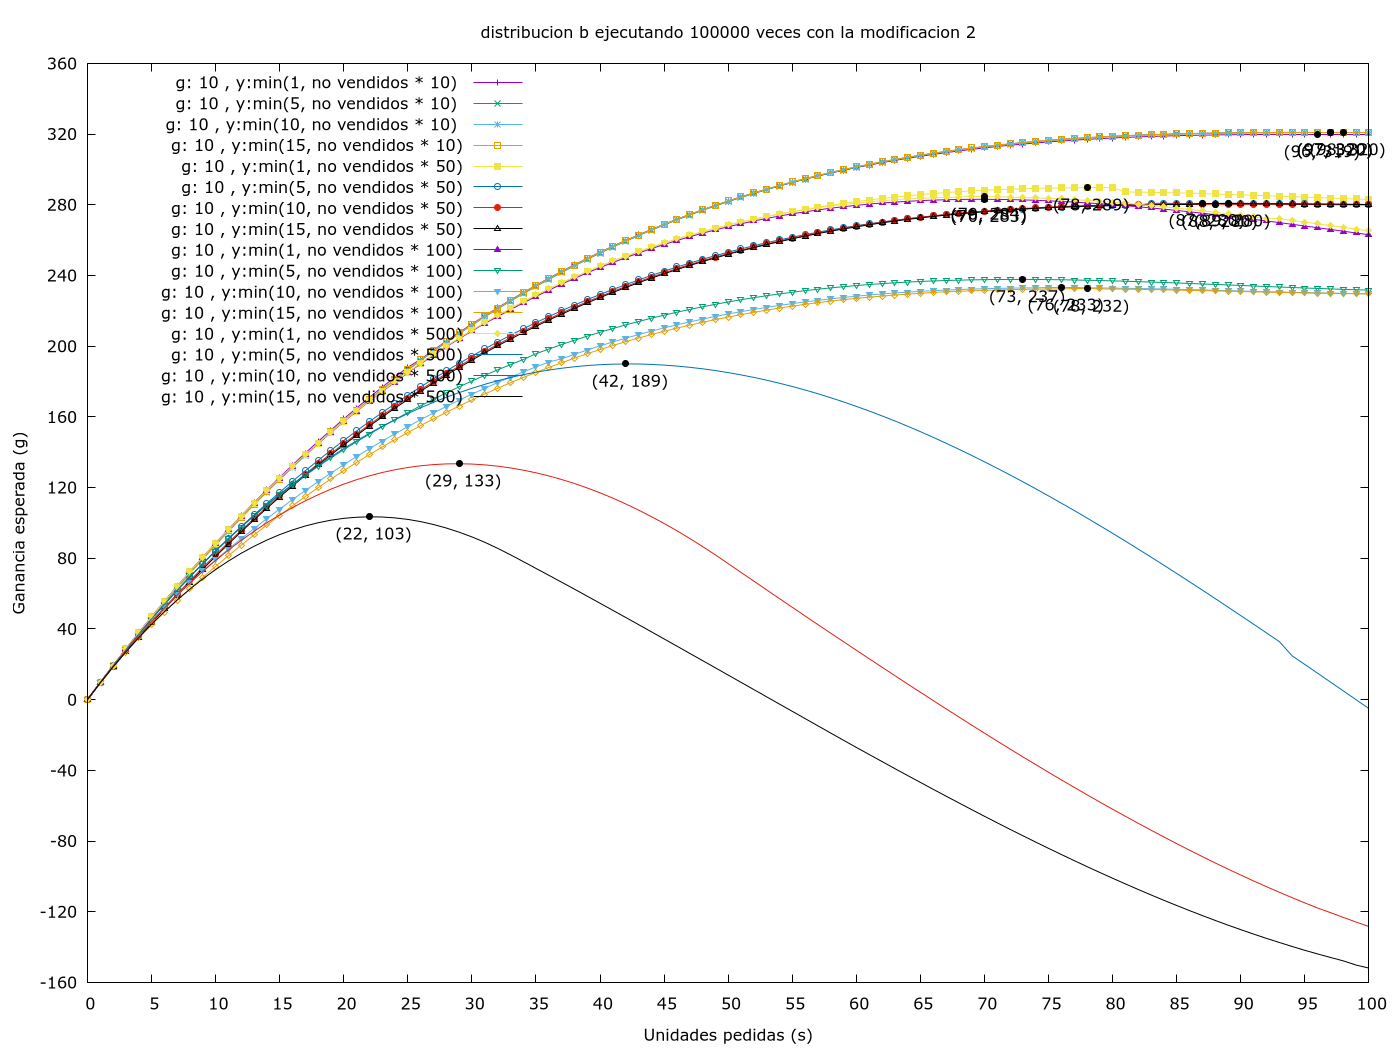
\includegraphics[scale = 0.2]{prob_b/datos_b_100000_2.png}
	\caption{Con 100000 repeticiones, la distribución b y la modificación 2.}
	\label{fig:ej1_a_100000}

\end{figure}

\begin{figure}[H]
	\centering
	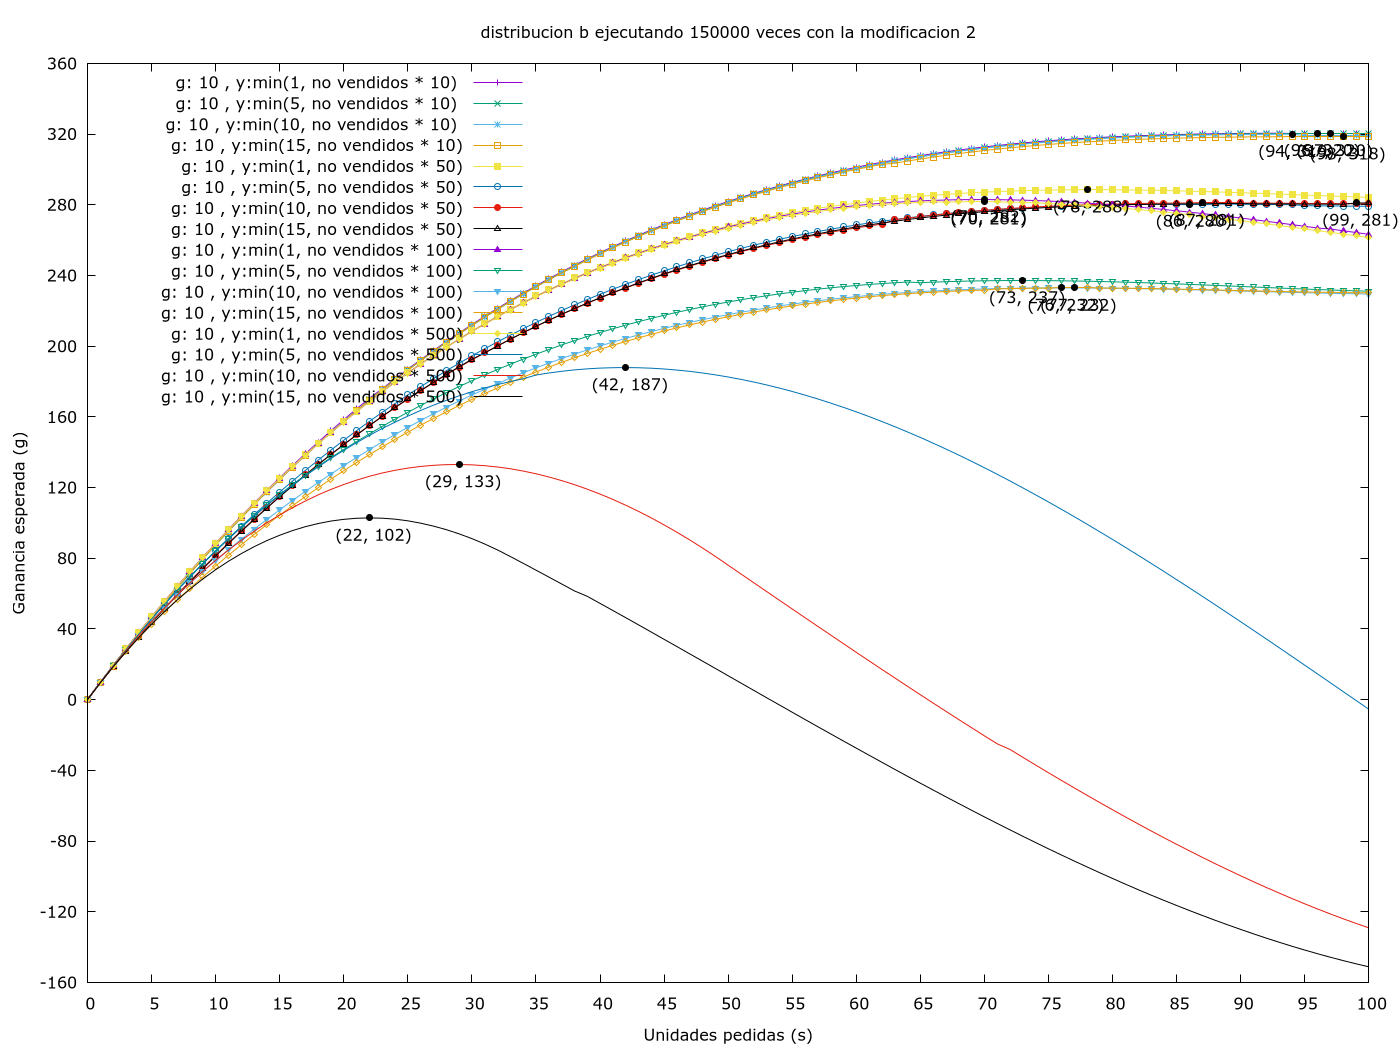
\includegraphics[scale = 0.2]{prob_b/datos_b_150000_2.png}
	\caption{Con 150000 repeticiones, la distribución b y la modificación 2.}
	\label{fig:ej1_a_150000}

\end{figure}


En esta ocasión, al utilizar la distribución proporcional, vemos como en los peores casos donde las unidades contratadas son tan altas y la demanda es muy poco probable en esos rangos, que si la penalización por unidades y el pago único es muy alto si nos puede llegar a tener pérdidas, sin emgargo eso solo ocurre en los casos extremos.

En la mayoría de los casos nos permite estabilizarnos a partir de las 50 unidades, y como en la mayoría de las situaciones anteriores, se nos sugiere ser más austeros si las penalizaciones son grandes y poder dar más margen si las penalizaciones son más bajas. La ventaja de este modelo es que tenemos dos vías de que la penalización sea baja, dando más posibilidad de encontrar un óptimo alto.

\subsubsection{Resultados obtenidos con la distribución c}

\begin{figure}[H]
	\centering
	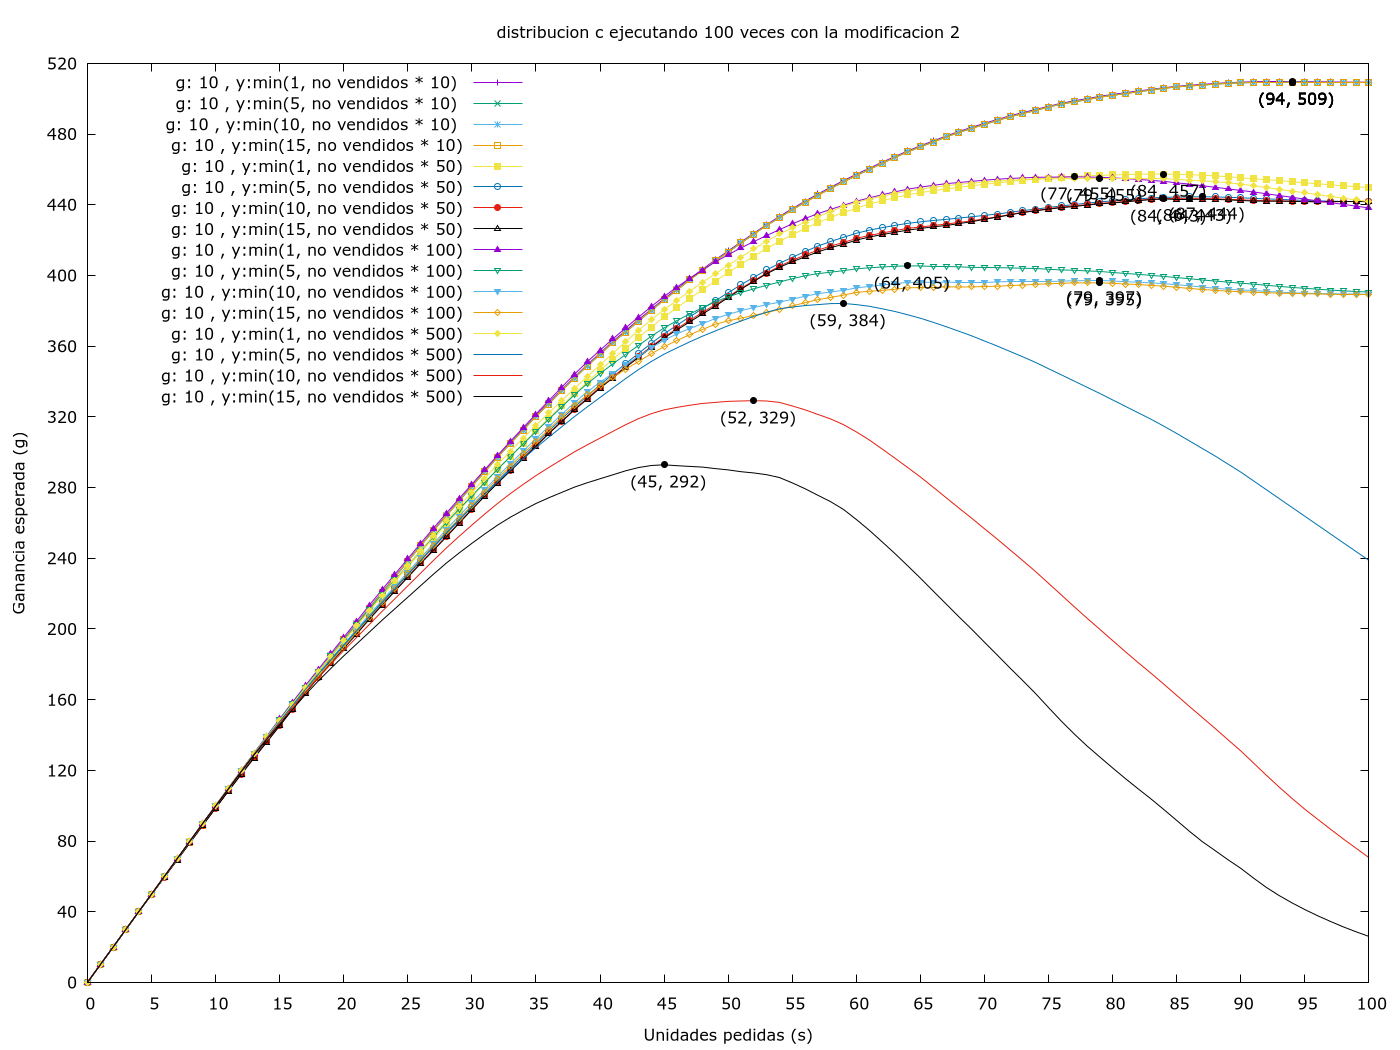
\includegraphics[scale = 0.2]{prob_c/datos_c_100_2.png}
	\caption{Con 100 repeticiones, la distribución c y la modificación 2.}
	\label{fig:ej1_a_100}

\end{figure}

\begin{figure}[H]
	\centering
	\includegraphics[scale = 0.2]{prob_c/datos_c_1000_2.png}
	\caption{Con 1000 repeticiones, la distribución c y la modificación 2.}
	\label{fig:ej1_a_1000}

\end{figure}

\begin{figure}[H]
	\centering
	\includegraphics[scale = 0.2]{prob_c/datos_c_5000_2.png}
	\caption{Con 5000 repeticiones, la distribución c y la modificación 2.}
	\label{fig:ej1_a_5000}

\end{figure}


\begin{figure}[H]
	\centering
	\includegraphics[scale = 0.2]{prob_c/datos_c_10000_2.png}
	\caption{Con 10000 repeticiones, la distribución c y la modificación 2.}
	\label{fig:ej1_a_10000}

\end{figure}

\begin{figure}[H]
	\centering
	\includegraphics[scale = 0.2]{prob_c/datos_c_100000_2.png}
	\caption{Con 100000 repeticiones, la distribución c y la modificación 2.}
	\label{fig:ej1_a_100000}

\end{figure}

\begin{figure}[H]
	\centering
	\includegraphics[scale = 0.2]{prob_c/datos_c_150000_2.png}
	\caption{Con 150000 repeticiones, la distribución c y la modificación 2.}
	\label{fig:ej1_a_150000}

\end{figure}

De nuevo se repite una situación similar a la modificación 1. Como esta distribución nos asegura un número relativamente alto de unidades vendidas, vemos como obtenemos grandes beneficios en cada óptimo, e incluso nos permite arriesgarnos sin llegar a tener pérdidas.

En resumen, el permitir tener dos vías de devolución nos añade la ventaja de poder cambiar entre una y otra, minimizando la pérdida y obteniendo unos óptimos de unidades a pedir mayores, y con mayor beneficio.


\section{Generadores de datos}

En este apartado de la práctica trabajaremos con generadores de datos. Desde la mejora de los generadores utilizado hasta ahora en la práctica, como el estudio e implementación de generadores de datos propio, aunque sean básicos.

\subsection{Mejoras de los generadores de datos}

En este apartado estudiaremos los generadores de datos dados. Estos generadores han sido implementados aplicando directamente el método de tablas de búsqueda, sin embargo no se han tenido en cuenta diversos aspectos que permitan una mejor ejecución.

Se nos proponen tres mejoras a los generadores de datos proporcionados:

\subsubsection{Reordenación de la tabla de búsqueda}

En esta primera mejora nos basamos en que para buscar en la tabla de búsqueda esta búsqueda se hace de forma secuencial, parando la búsqueda cuando encontramos el primer elemento que cumple la condición. Por este motivo, podemos intuir que si ordenamos la tabla de forma que se comprueben primero los valores con mayor probabilidad, se encontrará en menor tiempo el objetivo, por lo que se necesitará un tiempo menor.

Aun así, esta mejora solo funcionará en la distribución de probabilidad c, ya que la distribución a todos los valores tienen la misma probabilidad, por lo que es imposible ordenar algo que es equivalente para todos los valores, y en el caso de la distribución b ya esta ordenada de forma decrediente, ya que al ser proporcional a la demanda, la probabilidad va decreciendo según aumentamos el valor.


El caso en el que funcionará es la distribución de probabilidad c, ya que los valores más probables están en el centro de la tabla, mientras que los menos probables en los extremos.

Para implementar esta mejora en el código he utilizado una estructura propia, que cada instancia contiene la posición que le correspondería en la tabla original, y la probabilidad acumulada. De esta forma podemos poner en la primera posición de la tabla el valor que estaría en la mitad (el 50 en nuestro caso), con su correspondiente probabilidad, e ir rellenando la tabla del centro a los extremos, decrementando poco a poco la probabilidad de que aparezcan los elementos segun nos alejamos del centro. De esta forma obtendremos una tabla ordenada con los valores más probables al principio, en nuestro caso correspondería con una tabla que en la posición 0 tendría el elemento que estaría en la posición 50 en la original, en la 1 el 49, en la 2 el 51, y así sucesivamente.

Es importante almacenar el indice que le correspondería en la tabla original, ya que ese sería el valor de la demanda correspondiente.

Observamos como esta mejora produce una ventaja sustancial en el tiempo de ejecución:

\begin{figure}[H]
	\centering
	\includegraphics[scale = 0.2]{t_mejora1.png}
	\caption{Reordenando la tabla de búsqueda.}
	\label{fig:ej1_a_150000}

\end{figure}


\subsubsection{Implementación de la búsqueda binaria}

Como he comentado en el apartado anterior, la búsqueda en la implementación original se realiza de forma secuencial, que en el peor de los casos es de orden $O(n)$, sin embargo, como vimos en la asignatura de algorítmica, podemos implementar una búsqueda binaria que supondría un orden $O(log n)$, mejorando el tiempo de ejecución.

Esta mejora valdría sobre todas las distribuciones, ya que no depende de la forma de construir la tabla, si no de como recorrerla. El resultado sería el siguiente:

\begin{figure}[H]
	\centering
	\includegraphics[scale = 0.2]{t_mejora2.png}
	\caption{Aplicando una búsqueda binaria en lugar de secuencial.}
	\label{fig:ej1_a_150000}

\end{figure}

Como vemos, se mejoran los tiempos para todos los casos.

\subsubsection{Ejecución en tiempo constante para la distribución a}

Por último se nos pide implementar un método en el que la ejecución para la distribución a sea constante. Realmente, la distribución a, al ser una distribución uniforme, no es necesario implementar una tabla de búsqueda, ya que cada valor de la tabla de búsqueda corresponderá a $\frac{i}{n}$, siendo $i$ la posición en la tabla y $n$ el tamaño de la tabla. Por este motivo, en lugar de generar un número uniforme entre 0 y 1 y buscarlo en la tabla, podemos utilizar directamente $u * n$, siendo $u$ el número aleatorio uniforme entre 0 y 1. Por ejemplo, en nuestro caso, con una tabla de tamaño 100, si el uniforme obtenido es 0.66, buscaríamos en la tabla hasta encontrar ese elemento, pero es que sabemos que ese elemento está en la posición 66, ya que es $\frac{66}{100}$.

Tras esta mejora, el resultado es el siguiente:

\begin{figure}[H]
	\centering
	\includegraphics[scale = 0.2]{t_mejora3.png}
	\caption{Ejecución en tiempo constante para la distribución a.}
	\label{fig:ej1_a_150000}

\end{figure}



\newpage

\subsection{Implementación de generadores de datos básicos}

En esta sección se nos pide implementar dos generadores de datos congruenciales utilizando cuatro métodos distintos.

Como se explicó en teoría, el método se basa en una formula del estilo:

\[ x_{n+1} = f(x_{n}) \]

En concreto:

\[ x_{n+1} = (a \cdot x_{n} + c) \mod m \]

Donde $a$ es el multiplicador, $c$ el incremento, y $m$ el módulo.

Este tipo de generadores de datos ciclarán ya que solo dispone de un número finito de números. Al conjunto de números que cicla lo llamaremos periodo del generador, y nos interesará utilizar generadores con grandes periodos.

Para esta sección se nos pide crear dos generadores de datos congruenciales con las siguientes características:

\begin{enumerate}
	\item $a = 2061$, $c = 4321$ y $m = 10000$
	\item $a = 2060$, $c = 4321$ y $m = 10000$

\end{enumerate}


También se nos pide implementarlo utilizando cuatro tipos distintos de aritméticas.

\subsubsection{Utilizando aritmética entera}

En este caso para implementar el generador utilizaremos el operador $\%$ de C/C++.


\subsubsection{Utilizando aritmética real}


\subsubsection{Utilizando aritmética real corregida}



\subsubsection{Utilizando aritmética real con fmod}

% \begin{thebibliography}{9}
%
%
% \end{thebibliography}

\end{document}
